% !Mode:: "TeX:UTF-8"
%%% Local Variables:
%%% mode: latex
%%% TeX-master: t
%%% End:

\documentclass[type=master]{thuthesis}
% 选项:
%   type=[bachelor|master|doctor|postdoctor], % 必选
%   secret,                                   % 可选
%   pifootnote,                               % 可选(建议打开)
%   openany|openright,                        % 可选,基本不用
%   arial,                                    % 可选,基本不用
%   arialtoc,                                 % 可选,基本不用
%   arialtitle                                % 可选,基本不用

% 所有其它可能用到的包都统一放到这里了,可以根据自己的实际添加或者删除。
\usepackage{thuthesis}
\usepackage{bm}
\usepackage{algorithm}
\usepackage{algpseudocode}
\usepackage{makecell}

\usepackage{tikz}
\usetikzlibrary{arrows,shapes,positioning}

% 算法相关
\floatname{algorithm}{算法}
\makeatletter
\@addtoreset{algorithm}{chapter}% algorithm counter resets every chapter
\makeatother
\renewcommand{\thealgorithm}{\thechapter.\arabic{algorithm}}% Algorithm # is <chapter>.<algorithm>
\algnewcommand\algorithmicinput{\textbf{输入:}}
\algnewcommand\INPUT{\item[\algorithmicinput]}
\algnewcommand\algorithmicoutput{\textbf{输出:}}
\algnewcommand\OUTPUT{\item[\algorithmicoutput]}
\algnewcommand\algorithmicinit{\textbf{初始化:}}
\algnewcommand\INIT{\item[\algorithmicinit]}

%表格相关
\newcolumntype{Y}{>{\centering\arraybackslash}X}
\newcolumntype{I}{!{\vrule width 1.5pt}}

% 定义所有的图片文件在 figures 子目录下
\graphicspath{{figures/}}

% 可以在这里修改配置文件中的定义。导言区可以使用中文。
% \def\myname{薛瑞尼}
\begin{document}

%%% 封面部分
\frontmatter
\thusetup{
  %******************************
  % 注意:
  %   1. 配置里面不要出现空行
  %   2. 不需要的配置信息可以删除
  %******************************
  %
  %=====
  % 秘级
  %=====
  secretlevel={绝密},
  secretyear={2100},
  %
  %=========
  % 中文信息
  %=========
  ctitle={短波语音信号的质量评价算法及自动选路系统研究},
  cdegree={工学硕士},
  cdepartment={电子工程系},
  cmajor={信息与通信工程},
  cauthor={陈晔},
  csupervisor={谷源涛副教授},
  %cassosupervisor={陈文光教授}, % 副指导老师
  %ccosupervisor={某某某教授}, % 联合指导老师
  % 日期自动使用当前时间,若需指定按如下方式修改:
  cdate={二〇一七年六月},
  %
  % 博士后专有部分
  %cfirstdiscipline={计算机科学与技术},
  %cseconddiscipline={系统结构},
  %postdoctordate={2009年7月——2011年7月},
  %id={编号}, % 可以留空: id={},
  %udc={UDC}, % 可以留空
  %catalognumber={分类号}, % 可以留空
  %
  %=========
  % 英文信息
  %=========
  etitle={Study on Preprocessing Technique and Background Model in Drosophila Recognition and Behavior Analysis},
  % 这块比较复杂,需要分情况讨论:
  % 1. 学术型硕士
  %    edegree:必须为Master of Arts或Master of Science(注意大小写)
  %             “哲学、文学、历史学、法学、教育学、艺术学门类,公共管理学科
  %              填写Master of Arts,其它填写Master of Science”
  %    emajor:“获得一级学科授权的学科填写一级学科名称,其它填写二级学科名称”
  % 2. 专业型硕士
  %    edegree:“填写专业学位英文名称全称”
  %    emajor:“工程硕士填写工程领域,其它专业学位不填写此项”
  % 3. 学术型博士
  %    edegree:Doctor of Philosophy(注意大小写)
  %    emajor:“获得一级学科授权的学科填写一级学科名称,其它填写二级学科名称”
  % 4. 专业型博士
  %    edegree:“填写专业学位英文名称全称”
  %    emajor:不填写此项
  edegree={Master of Science},
  emajor={Information and Communication Engineering},
  eauthor={Hou Qi},
  esupervisor={Associate Professor Gu Yuantao},
  %eassosupervisor={Chen Wenguang},
  % 日期自动生成,若需指定按如下方式修改:
  edate={April, 2016},
  %
  % 关键词用“英文逗号”分割
  ckeywords={果蝇, 背景模型, 行为分析},
  ekeywords={Drosophila, Background Model, Behavior Analysis}
}

% 定义中英文摘要和关键字
\begin{cabstract}
  动物行为学研究是生物学研究的一个重要领域,动物行为学通过观察、计数研究动物的行为。果蝇的基因结构简单、身体结构简单,成为动物行为学研究中的重点研究对向。果蝇行为学研究需要分析大量的果蝇视频数据,手工标定需要花费大量的人力成本,且手工标定可能存在标准不一致等问题,用计算机自动分析果蝇的行为成为一个可行解决方案。目前已经存在自动分析果蝇行为的研究。果蝇行为识别的主要流程包括果蝇活动台提取、果蝇身体轮廓提、果蝇特征提取、行为模式识别等步骤。目前的研究一般受限于特定的实验条件和拍摄环境,往往难以适应其他实验环境。其中,果蝇轮廓提取步骤往往是其中的制约因素。此外,果蝇活动台提取步骤也限制了整个流程自动化的程度。为此,本文提出一种特定排列模式下的果蝇活动台提取算法和一种基于背景模型的轮廓提取算法。主要工作可以概括为以下几个方面:

  首先,本文提出一种特定排列模式下的果蝇活动台轮廓提取算法。通过圆检测等形状检测方式提取活动台的位置和大小,进而根据果蝇活动台的排列方式,对果蝇活动台的位置进行进一步的调整。

  其次,本文提出一种基于背景模型的果蝇轮廓提取算法,可以从视频中提取果蝇的身体和翅膀。算法采用单高斯模型作为背景模型,通过亮度畸变区分果蝇翅膀和身体。初步建模后分离果蝇身体和活动台背景;然后在对活动台单独进建模的基础上,得到最终的背景模型。

  然后,在背景模型的基础上,进行果蝇打架行为分析,验证了本文提出的算法的有效性。

  最后,搭建果蝇行为识别网站,并介绍果蝇行为识别软件的程序部分和网站部分,以及网站的基本使用说明。

  本文提出的基于特定排列模式的果蝇活动台算法提高了果蝇自动分析的自动化程度;基于背景模型的果蝇轮廓提取算法具有较好的鲁棒性,可以适用于不同拍摄环境,有助于提高自动化果蝇行为分析的适用范围。此外,该模型还可以应用于动物行为学中对其他动物的研究。


\end{cabstract}

% 如果习惯关键字跟在摘要文字后面,可以用直接命令来设置,如下:
% \ckeywords{\TeX, \LaTeX, CJK, 模板, 论文}

\begin{eabstract}

In biology research, ethology is an important area. By observing the behavior of animals, ethologists get the internal mechanism of animals. Drosophila has a simple genetic structure as well as a simple body structure, which makes it an important role in ethology. In traditional research, much manpower is needed to watch the videos and count the behaviors. Also, there may be different standards for behavior detection, which makes it hard to generalize. With the development of computer vision and machine learning, analyzing the fly video by computer becomes possible.

The main procedure includes drosophila chamber extraction, drosophila body contour extraction, drosophila feature extraction, and drosophila behavior pattern recognition. But the current study is generally limited by specific environments, and cannot generalize to other laboratory circumstance. Drosophila contour extraction step is often the restrictive factors, followed by drosophila chamber extraction step. To solve this problem, we propose a method to extract drosophila chambers based on the specific layout pattern. For the contour extraction step, we propose a drosophila contour extraction algorithm based on background model. The main work can be summarized as follows:

Firstly, this paper presents a drosophila chamber extraction algorithm based on specific layout pattern. First extract the chambers by shape detection method such as hough circle detection, then cluster the shapes to get the position of chambers, then adjust the position according to the layout of the chambers with transformation of coordinates.

Secondly, this paper presents a drosophila contour extraction algorithm based on background model, which extracts the body and wings of drosophila from the video. The algorithm uses a single Gaussian distribution as the background model, and distinguishes the drosophila wings and body by luminance distortion. After the preliminary background modeling, we can separate the drosophila body from the containers. Then we do background modeling on the container only, which makes a better background model for drosophila contour extraction.

Then, we analyze the fly fighting behaviors based on the algorithm, and it turns out to be effective.

Finally, we build a website that provide fly behavior analysis service, also we make a detailed introduction to the DetectFly software and the website, as well as the basic instructions for the website.

In conclusion, the drosophila chamber extraction algorithm reduce the manual operation in drosophila analysis. The contour extraction algorithm proves to be robust in different videos from different cameras, which helps to improve the application scope of  automated drosophila behavior analysis. In addition, the model can be applied to animal studies in other animals.

\end{eabstract}

% \ekeywords{\TeX, \LaTeX, CJK, template, thesis}

% 如果使用授权说明扫描页,将可选参数中指定为扫描得到的 PDF 文件名,例如:
% \makecover[scan-auth.pdf]
\makecover

%% 目录
\tableofcontents

%% 符号对照表
% !Mode:: "TeX:UTF-8"
%%% Local Variables:
%%% mode: latex
%%% TeX-master: t
%%% End:

\begin{denotation}[3cm]
\item[$I$]  视频中的图像帧
\item[$param_1$]  Hough圆检测的Canny算子阈值参数
\item[$param_2$]  Hough圆检测的累加器阈值参数
\item[$A$]  图像坐标系向理想坐标系的变换矩阵
\item[$B$]  理想坐标系向图像坐标系的变换矩阵
\item[$\textrm{M}_1$] 简单单高斯背景模型
\item[$\textrm{M}_2$] 果蝇活动台的精确背景模型
\item[$\mu$]    背景模型$\textrm{M}_1$中视频帧的均值
\item[$\sigma^2$]   背景模型$\textrm{M}_1$中视频帧的方差
\item[$\alpha$] $\textrm{M}_1$中视频帧的亮度畸变
\item[$\textrm{RMS}(\alpha)$] $\textrm{M}_1$中视频亮度畸变的均方差
\item[$\mu'$]   背景模型$\textrm{M}_2$中活动台的均值
\item[$\sigma^{\prime 2}$] 背景模型$\textrm{M}_2$中活动台的方差
\item[$\alpha'$] $\textrm{M}_2$中视频帧的亮度畸变
\item[$\textrm{RMS}(\alpha')$] $\textrm{M}_2$中视频亮度畸变的均方差
\item[$I_{body}$]    果蝇身体的二值图像
\item[$I_{wing}$]    果蝇翅膀的二值图像
\item[$\tau_{body}$] 提取果蝇身体的阈值
\item[$\tau_{wing}$] 提取果蝇翅膀的阈值
\item[$a$]    视频中的果蝇身体长度的一半
\item[$b$]    视频中的果蝇身体宽度的一半
\item[$\vec{\bm p}$]    果蝇特征点坐标
\end{denotation}



%%% 正文部分
\mainmatter

\tikzstyle{block} = [rectangle, draw, text width=15em,  text centered, rounded corners, minimum height=3.5em]
\tikzstyle{arrow} = [thick, draw, -latex']

%引言
% !Mode:: "TeX:UTF-8"
%%% Local Variables:
%%% mode: latex
%%% TeX-master: t
%%% End:

\chapter{引言}
\label{chapter:introduction}

\section{研究背景}

短波通信又称高频通信,是指使用频率范围在高频(HF)的无线电进行通信的方式\cite{董彬虹2007短波通信的现状及发展趋势}。短波通信主要利用天波电离层反射,所以无需中继站即可实现远距离通信,具有机动性强、设备成本低、对基础设施依赖小的优点,因此被广泛应用于广播、军事和抢险救灾等领域。

而同时,短波通信的缺陷也非常突出,因为受电离层变化和多径传播等因素的影响,短波通信的信道非常不稳定,导致其通信质量起伏较大,影响通信的稳定性。应对这一问题,军事中应用短波语音进行地空通信时,目前有一种解决方案:如图~\ref{fig:sys_struct}所示,在地面不同地点建立多个短波信号接收基站,接收来自空中飞机的短波语音。再将这多路信号汇总到一起,由人工选择一路质量最优的信号接入给地面指挥人员。人工选择需要的人工成本高,且稳定性和可靠性都不高,亟待使用算法代替人工。本文旨在通过对一系列算法及系统的研究,使用算法替代该方案中的人工选择步骤。

\begin{figure}
\centering
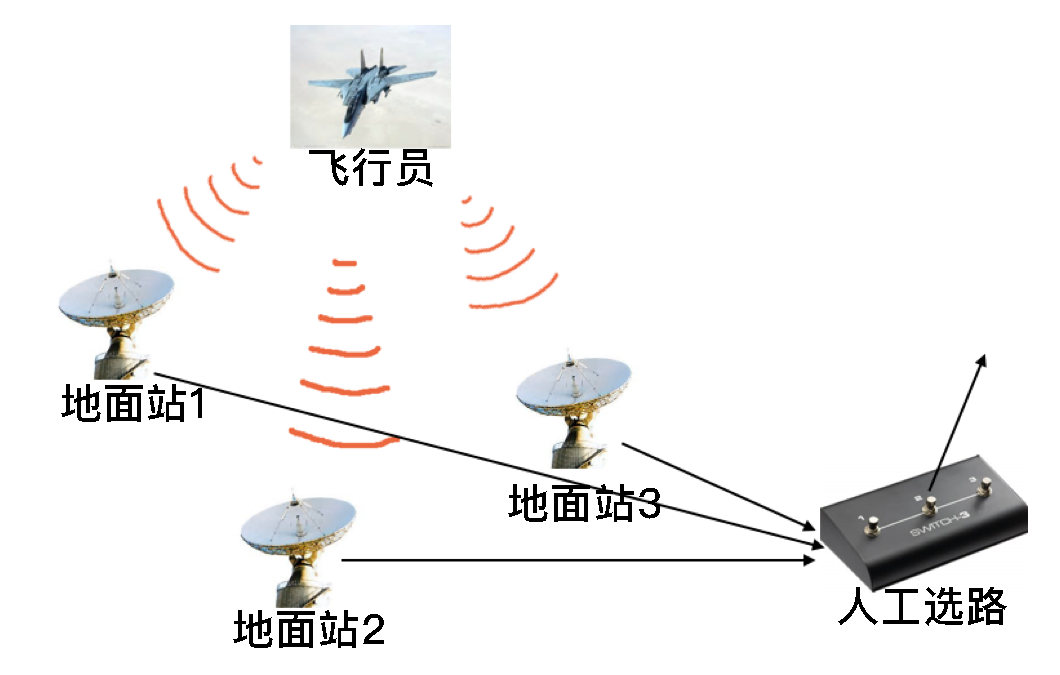
\includegraphics[width=0.8\textwidth]{sys_struct}
\caption{军事应用中的一种地空短波通信系统\label{fig:sys_struct}}
\end{figure}

\section{研究现状}


\subsection{背景模型及其在果蝇身体检测中的应用}


\section{研究目标和研究内容}

本文的主要目标在于研究果蝇活动台分割算法和果蝇轮廓提取算法,提升算法的鲁棒性,提升果蝇行为识别算法的应用范围。本文的研究内容主要包括:
\begin{enumerate}
\item 针对现有果蝇活动台提取算法的精确度较低的问题,本文引入了果蝇活动台的排列模式,通过将图像中的活动台和理想排列模式之间建立一一映射,去除果蝇活动台提取过程中的噪声。此外,对于不按照固定模式排列的果蝇活动台,引入自适应机制,减少该步骤中的人工干预;
\item 果蝇行为视频的实验环境和拍摄条件差异给果蝇轮廓提取带来很大的困难,针对此问题,本文提出一种果蝇轮廓提取算法,采用单高斯模型作为背景模型,通过亮度畸变区分果蝇翅膀和身体。初步建模后分离果蝇身体和活动台背景;然后在对活动台单独进建模的基础上,得到精确的背景模型用于轮廓提取。
\item 创建果蝇行为识别网站,对果蝇研究单位提供果蝇视频分析服务。
\end{enumerate}

\section{论文结构和内容概述}

本文剩余部分的结构如下所示:

第2章主要介绍短波语音客观质量评价算法。介绍了两种客观评价算法,一种是基于语谱图噪音模型的算法,另一种是基于人工神经网络自编码器的算法。前者根据短波语音的噪音特征设计,对于短波语音的质量评价效果非常好,但是算法针对性太强,迁移到其他领域的语音信号时,需要重新分析对应的噪音特征;而后者通过自编码器学习纯净语音信号的语谱特征,可以方便地迁移到其他领域。

第3章主要介绍多路短波语音自动选路系统。首先介绍了多路语音时间对齐算法,然后介绍了基于此算法以及第2章介绍的客观评价算法的自动选路系统。

第4张介绍了语音质量在线主观评价辅助系统,首先介绍了系统的功能和使用方法,然后介绍了系统开发和部署环境及运行原理。

第5章介绍了实验的情况。通过两组实验分别验证了第2章所提算法及第3章所提系统的实际效果,在短波语音数据集上对比了本文所提算法与两种标准质量评价算法的表现。

第6章对本文工作进行总结,并对将来可能的研究方向进行展望。


\chapter{短波语音客观质量评价算法}
\label{chap:algorithms}

为了能够从多路短波语音中自动切换选择,需要使用算法对各路短波语音的质量进行评价。由于系统没有原始语音作为参考,所以需要的客观质量评价算法是单端的客观评价算法。现有的语音客观质量评价算法主要针对VoIP应用、语音编解码系统、语音降噪系统等场景,这些场景中的语音质量相较短波语音要好,信噪比较高。直接将现有的算法应用到短波语音上难以取得良好的评价结果。所以本章提出了两种可用在短波语音上的客观质量评价算法

\section{基于语谱图噪音模型的客观质量评价算法}

\subsection{启发性思路} \label{section:alg1-1}

语谱图是一种从频域对语音信号进行分析的工具,将语音信号转换到频域进行分析,需要使用短时傅里叶变换(STFT)。给定一个时间宽度很短的窗函数,语音信号的STFT定义为\ref{eq:stft}

\begin{equation}\label{eq:stft}
F_{STFT}(t, f) = \int_{-\infty}^{+\infty}x(u)g^*(u-t)e^{-j2\pi fu}du
\end{equation}

由于窗函数在时域有限,使得短时傅里叶变换具有局部特性,能够反映指定时刻的局部频谱信息。
实际应用中,需要使用离散化的短时傅里叶变换,取$t=mT, f=nF$,其中$T$和$F$分别为时间和频率的采样间隔,$m,n=0,1,2,...,M-1$,$M$是采样点数。则离散形式的STFT为\ref{eq:dstft}

\begin{equation}\label{eq:dstft}
F_{STFT}(m, n) = \sum_{k=0}^{N-1}x(kT)g^*((k-m)T)e^{-j2\pi nk/N}
\end{equation}

$F_{STFT}(m, n)$反映的是$mT$时刻,$nF$频率附近的局部频谱信息。

根据对于人耳听觉特性的一些研究,人耳对于声音信号的相位特性并不敏感,但是对于幅度特性敏感,并且人耳对于声音响度的感受是与信号能量的对数成正比的。所以对离散短时傅里叶变换得到的结果,只保留幅值能量,并进一步做取对数的处理,得到的二维信息可以用图像展示,称之为语谱图,定义为\ref{eq:log_dstft}

\begin{equation}\label{eq:log_dstft}
G(m, n) = log(|F_{STFT}(m, n)|^2)
\end{equation}

语谱图反映了语音信号在不同时间、不同频率上的能量大小,承载了语音所包含的信息。高质量语音的语谱图上有着清晰的结构特征,包括基音部分的能带,各种高次谐波的能带;而带有噪音的语谱图则没有模糊不清。在短波语音信号上亦是如此。如图~\ref{fig:timefreq}所示,从左到右是质量由低到高五组短波语音的语谱图,分别对应主观评分1-5分。从语谱图上可以看到条带状的语音部分越来越突出和明显。图~\ref{fig:timefreq-thr0.3}是由图~\ref{fig:timefreq}中各个语谱图以0.3为阈值转化为二值图像的结果,图中可以更加明显的看出质量越好的语音信号,条带状的纯净语音部分越清楚,而质量较差的语音信号,则因为存在噪音连成模糊的一片。

\begin{figure}
\centering
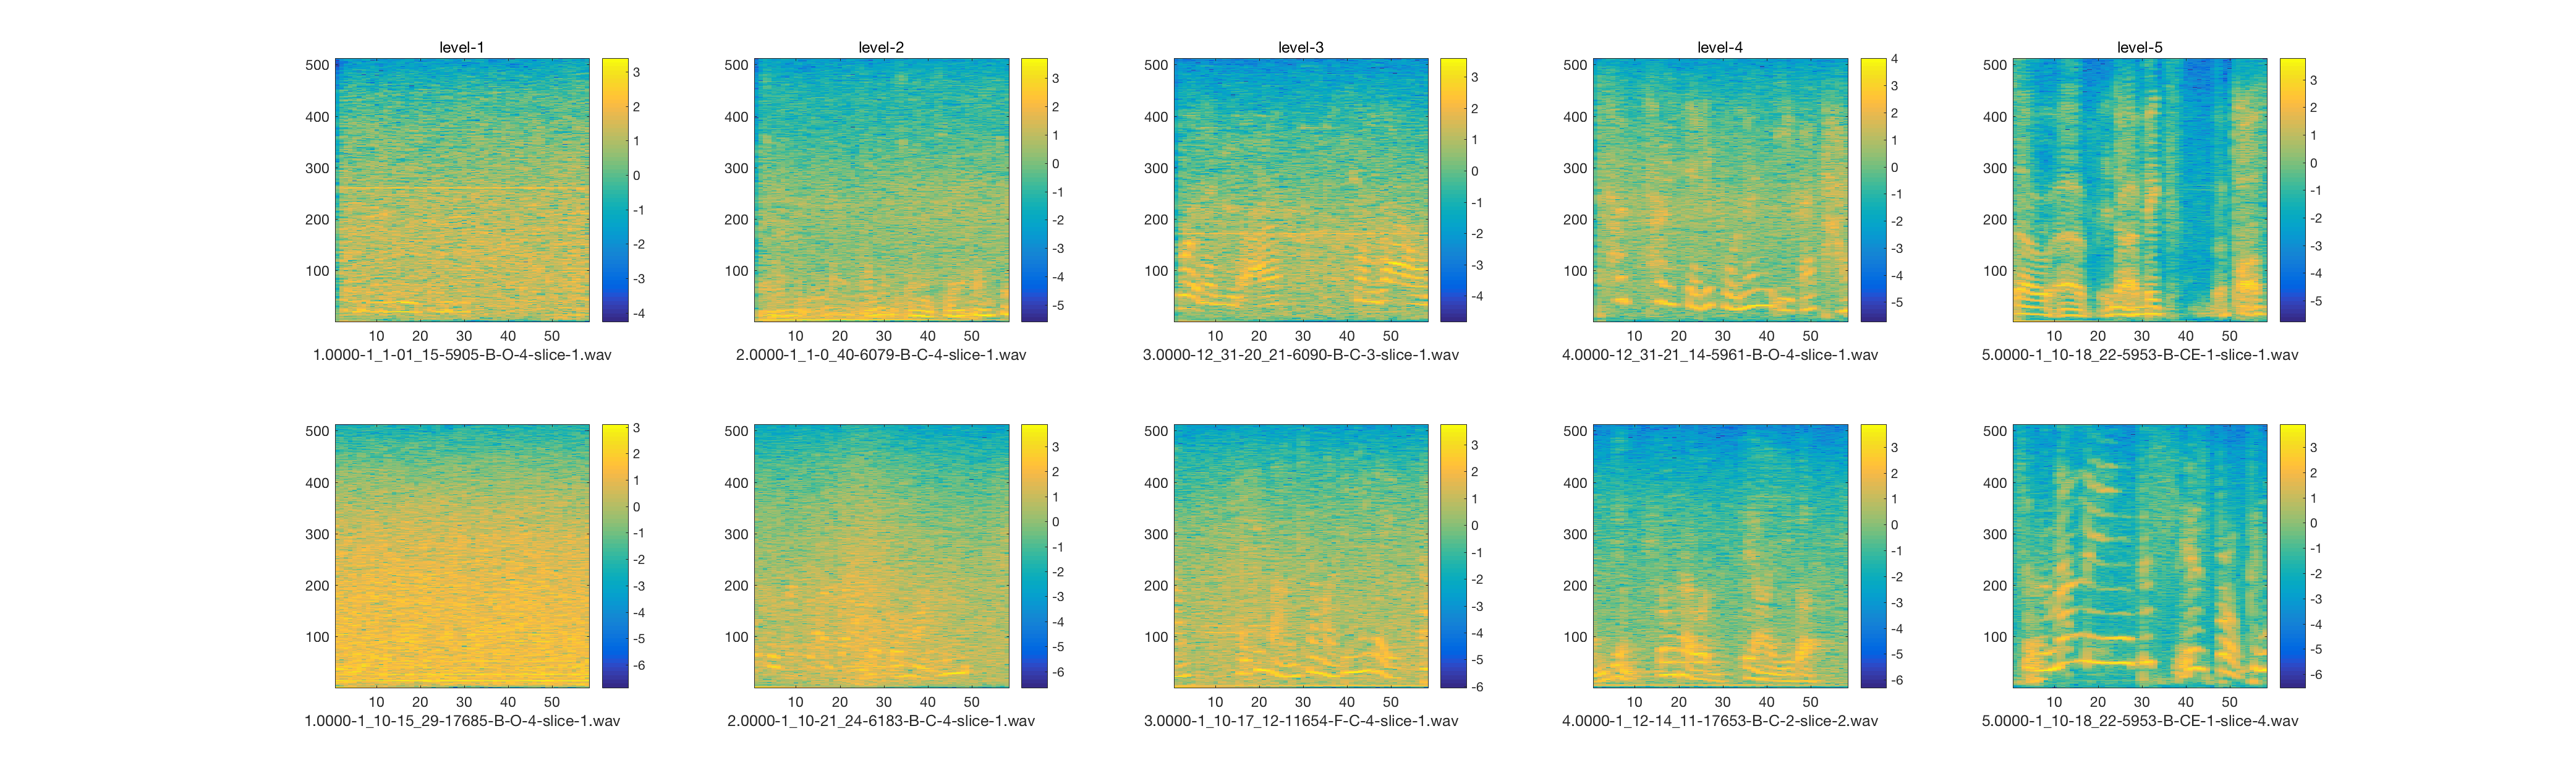
\includegraphics[width=1\textwidth]{timefreq}
\caption{不同质量的短波语音语谱图\label{fig:timefreq}}
\end{figure}

\begin{figure}
\centering
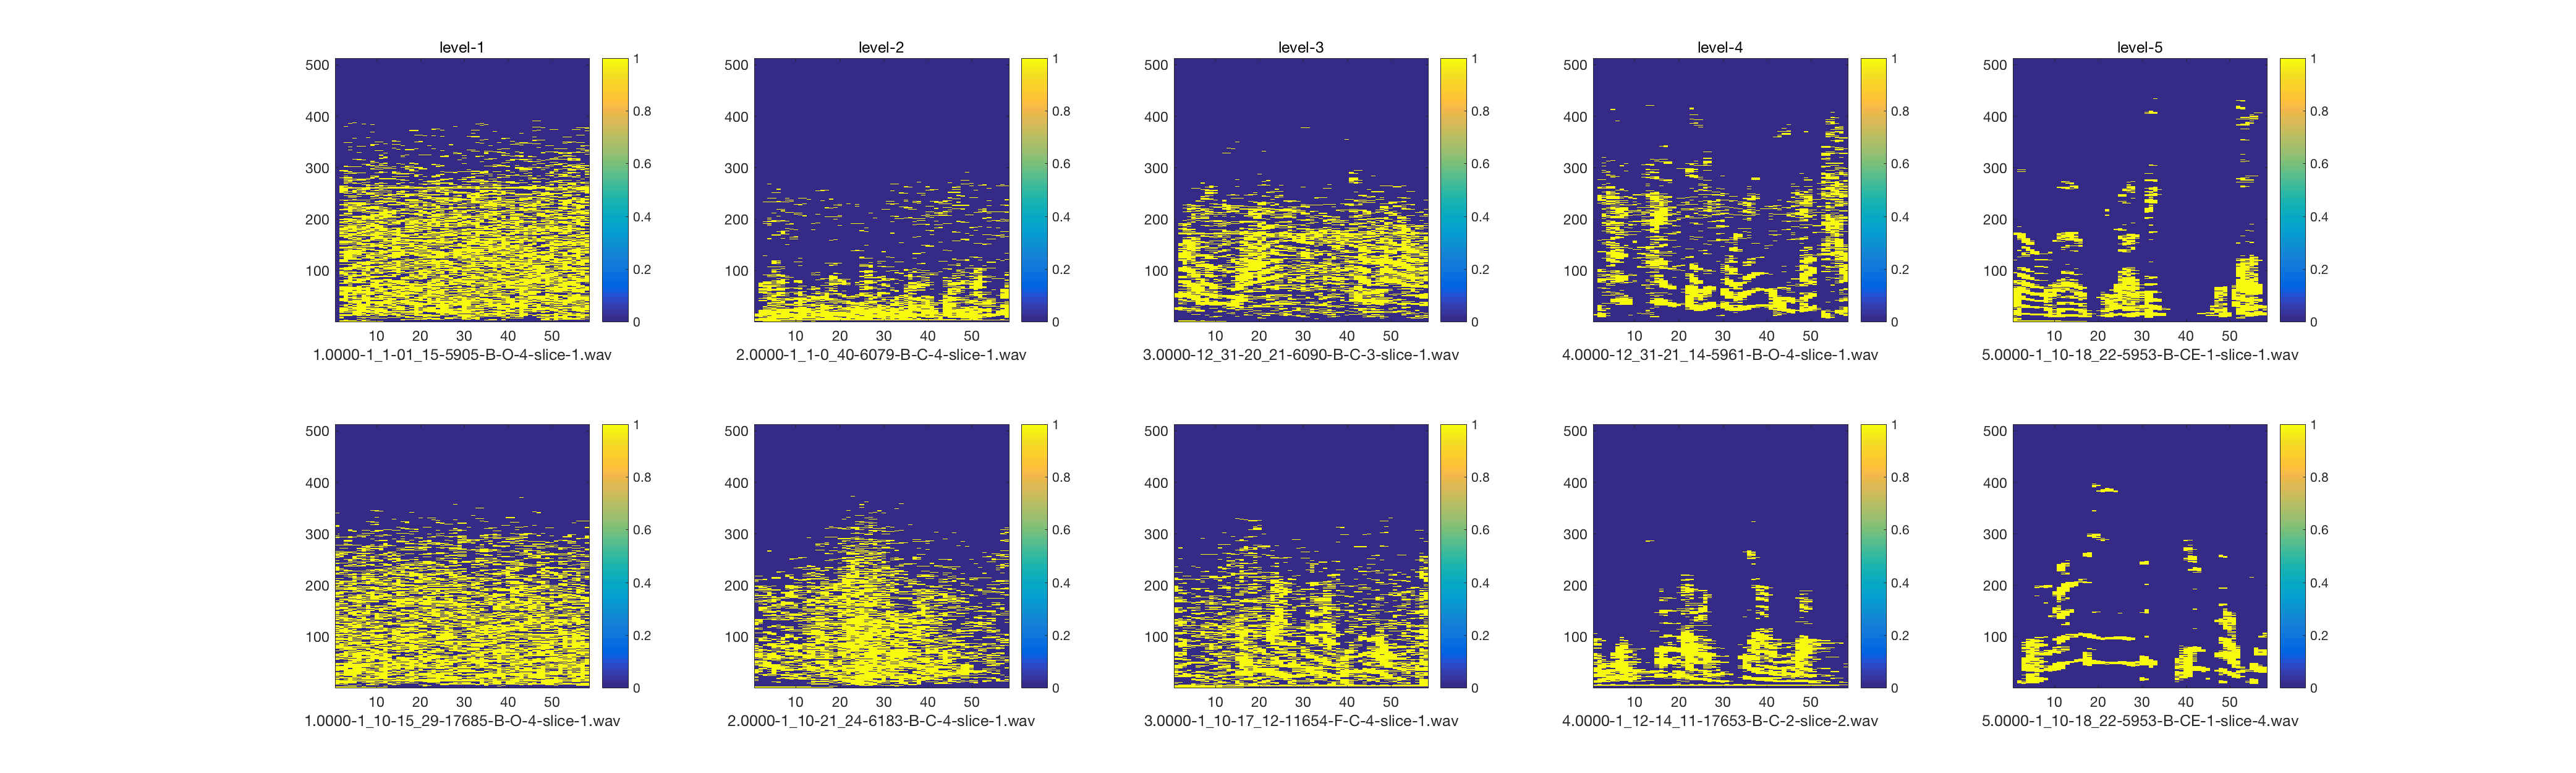
\includegraphics[width=1\textwidth]{timefreq-thr}
\caption{不同质量的短波语音二值化语谱图\label{fig:timefreq-thr0.3}}
\end{figure}

\begin{figure}
\centering
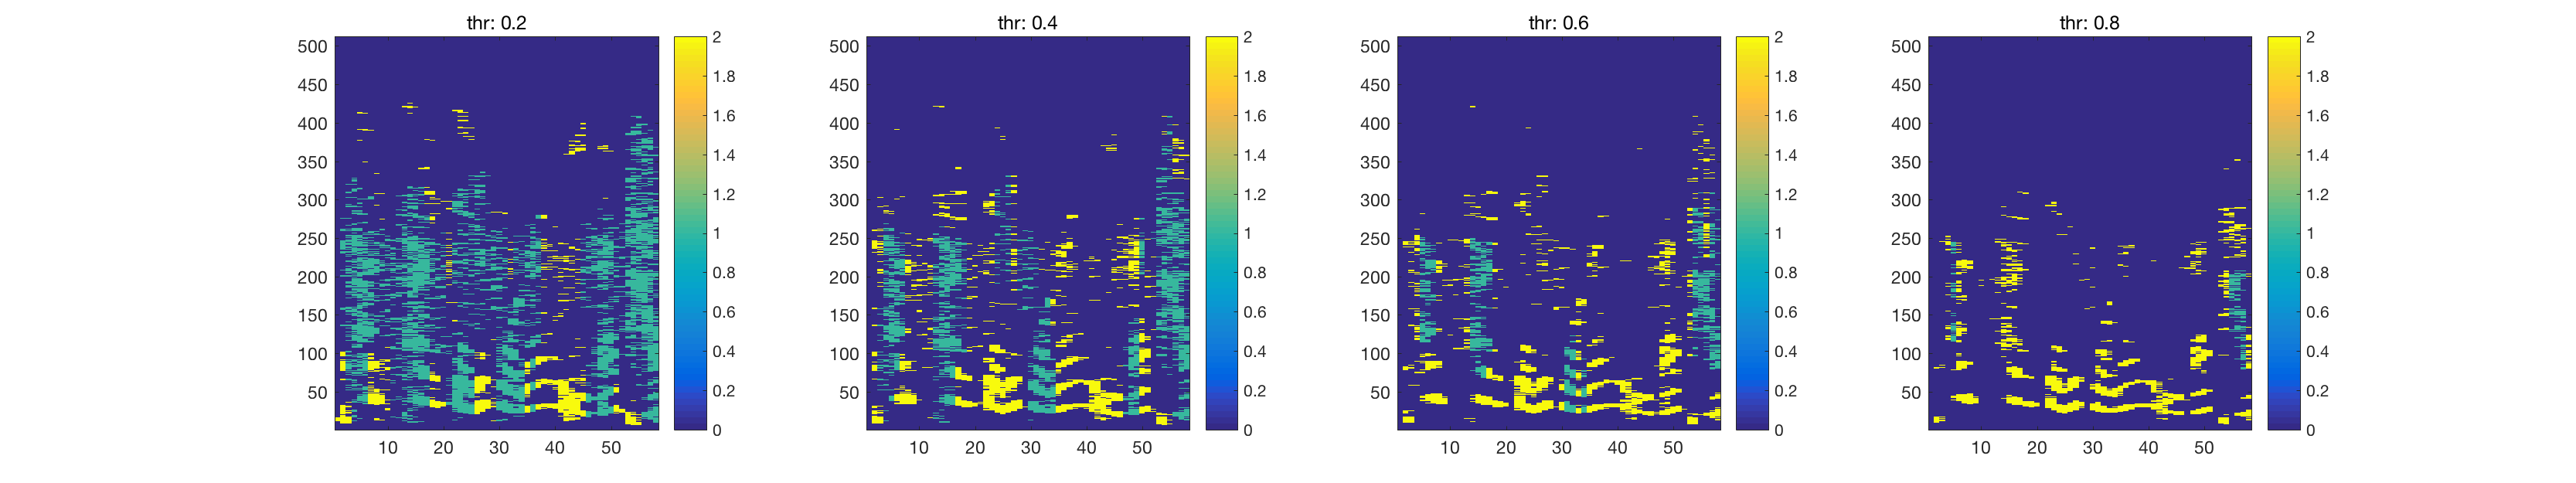
\includegraphics[width=1\textwidth]{timefreq-thrs-label}
\caption{不同阈值的二值化语谱图\label{fig:timefreq-thrs-label}}
\end{figure}

进一步地,从中选出一个语音信号,分别以0.2, 0.4, 0.6, 0.8为阈值绘制其二值化语谱图,如图~\ref{fig:timefreq-thrs-label}所示。而图中绿色区域是程序通过建立噪音模型,使用一些特征标注出的被噪音干扰的区域。可以发现,在阈值较低时,因为噪音部分留在了图上,所以看上去是大片大片的噪音;而当阈值逐渐升高,噪音部分逐渐从图上消失,留下的就都是纯净的语音信号。若当阈值超过某一阈值t时,语谱图上某一点不再被噪音干扰,那么这一点实际能量比t高出的部分就表征了这一点语音信号相对于噪音部分高出的强度。本文称之为该点的语音分辨率,计算语谱图上所有点的语音分辨率,进而得出语音质量的客观评价分。

\subsection{算法流程}

本小节介绍基于语谱图噪音模型的客观质量评价算法的具体流程,算法总体流程示意如图~\ref{fig:flowchart}所示。一维的短波语音信号经过加窗傅里叶变换得到二维的频域信号,其中横轴为时间维度,纵轴为频率维度。随后用不同阈值将语谱图转化成多张二值图像,再各个二值图像上使用图像处理的一些方法区分噪音区域和语音区域。再此基础上得到原始语谱图上各个点的“语音分辨率”,进而得到对于短波语音的客观评价分数。下面详细介绍各个步骤的内容。

\begin{figure}
\centering
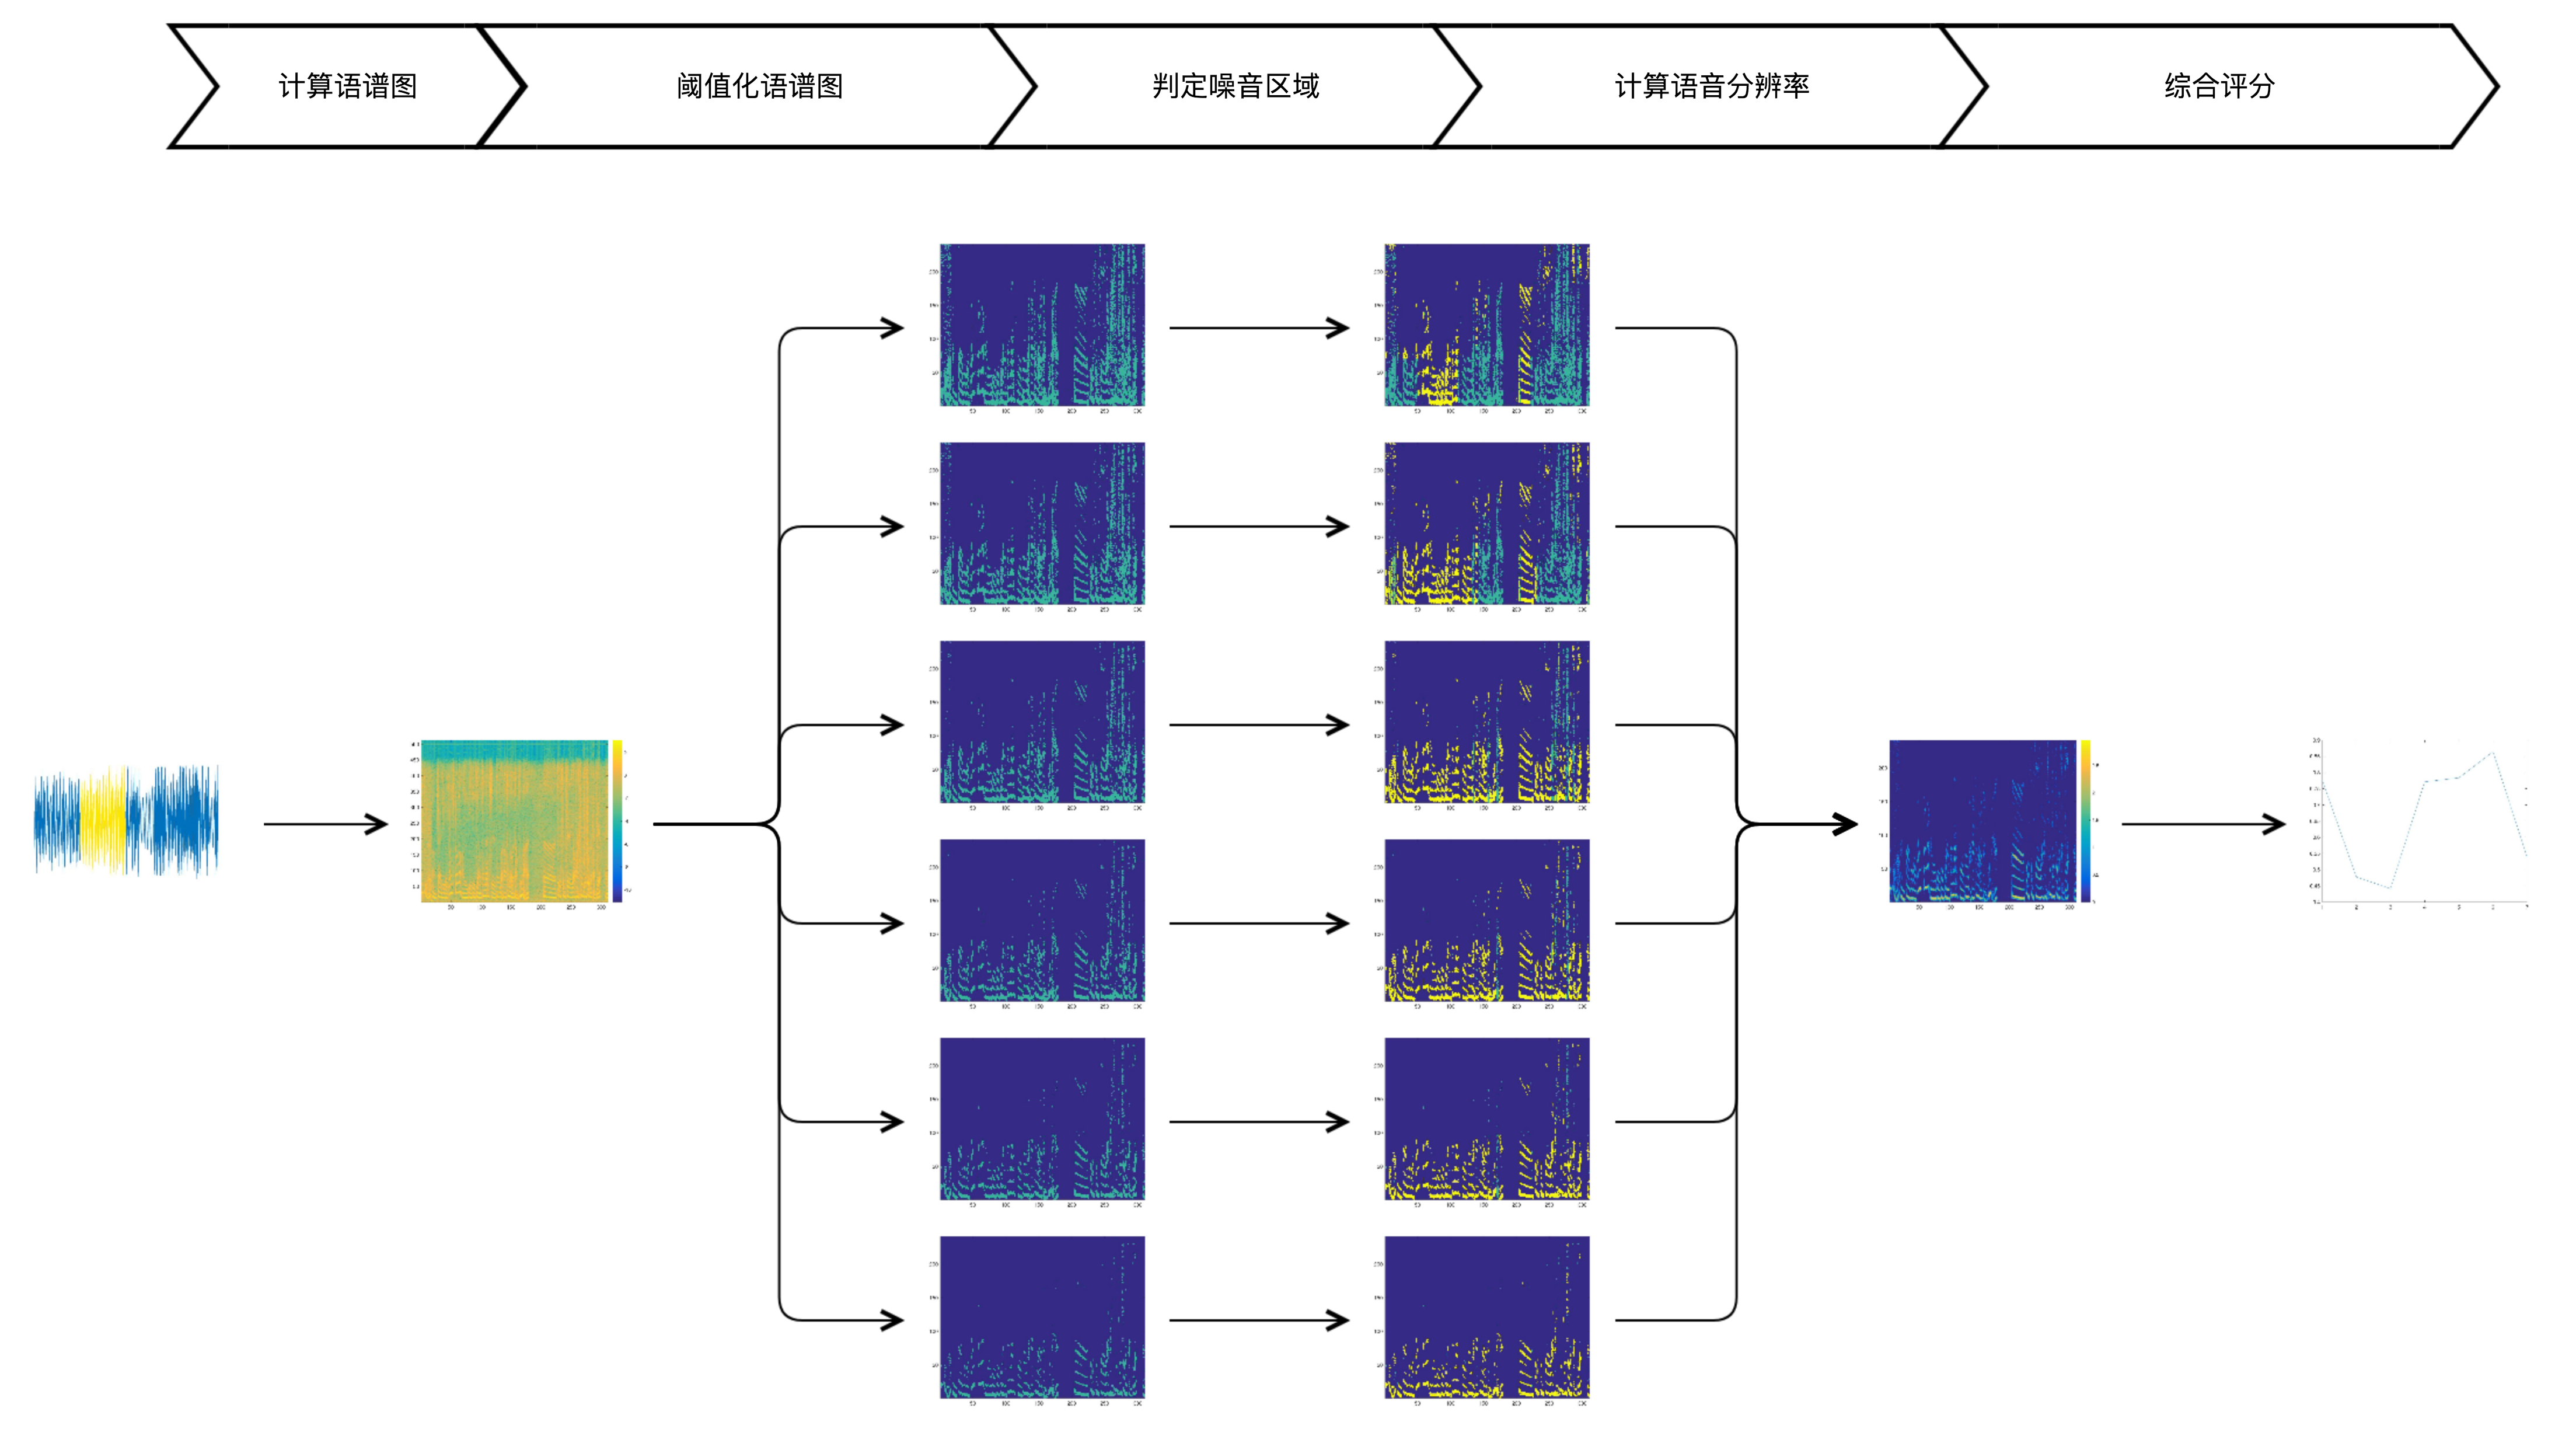
\includegraphics[width=0.8\textwidth]{flowchart}
\caption{基于语谱图噪音模型的客观质量评价算法流程\label{fig:flowchart}}
\end{figure}

首先根据上一小节介绍的语谱图的内容,使用短时傅里叶变换获得短波语音信号的语谱图$G(m,n)$。

取一系列的阈值$t_1<t_2<t_3<...<t_N$,我们进一步对语谱图做阈值化处理形成二值的语谱图,阈值化语谱图定义为

\begin{equation}\label{eq:thr_tf}
G_i(m, n) = \left\{
    \begin{array}{rcl}
    1, && {G(m,n)>t_i} \\
    0, && {G(m,n)\leq t_i}
    \end{array} \right.
\end{equation}

根据短波语音语谱图上的噪音模型,使用以下几种条件来判定噪音区域:
\begin{enumerate}
\item 区域$A_1$:语谱图上通过霍夫变换检测的与水平夹角小于1度的直线。
\item 区域$A_2$:某一长宽各大于一定阈值的范围内,$G_i(m,n)=1$的点数占据面积的80\%以上。
\item 区域$A_3$:某一连通域面积比上该连通域占据的宽度,其值超过一定阈值。
\item 区域$A_4$:某一连通域,其面积小于一定阈值。
\end{enumerate}

标注后的语谱图
\begin{equation}\label{eq:label_tf}
G_i^*(m, n) = \left\{
    \begin{array}{rcl}
    0, && {G_i(m,n)=0} \\
    1, && {G_i(m,n)=1且(m,n)\in \bigcup_{k=1}^4 A_k} \\
    2, && {else}
    \end{array} \right.
\end{equation}

定义集合
\begin{equation}\label{eq:collection}
\Psi(m,n)={i|G_i*(m,n)=2}
\end{equation}

定义语音分辨率
\begin{equation}\label{eq:resolution}
D(m,n) =  \left\{
    \begin{array}{rcl}
    0, && {\Psi(m,n)=\emptyset} \\
    G(m,n) - \min_{i\in\Psi(m,n)}t_i, && {\Psi(m,n)\neq\emptyset}
    \end{array} \right.
\end{equation}

对语音分辨率取平均得到客观评价分数
\begin{equation}\label{eq:score}
S = \frac{\sum D(m,n)}{\sum G_1(m,n)}
\end{equation}

为保证阈值化语谱图包含有效信息,阈值参数的取值范围应该是。一种简单的选取方法是直接在到选取$N$等分点。
为了尽量细致地刻画语谱图的特征,阈值的选取应该尽量密集,但同时算法的时间复杂度正比于阈值的数量,密集的阈值也会导致更高的计算复杂度。所以阈值的选取应当使用尽量少的阈值尽量高效地刻画语谱图的特征,上述选取方法显然不够高效。一方面,阈值很接近$\min{G(m,n)}$或者$\max{G(m,n)}$时,阈值化语谱图上的点非常少或者非常多,能提供的信息量很少。另一方面因为阈值增加同样大小,阈值化语谱图上的点数增加可能差异很大。均匀地选取阈值,会导致在有些区间,连续的几张阈值化语谱图过于相像而浪费计算资源,有些区间,阈值化语谱图又变化太快导致刻画不够细致。

一种改进的动态选取阈值的方法如下:先在5\%至20\%之间均匀选定一系列比例$\alpha_1,\alpha_2,\alpha_3,...,\alpha_N$,再计算得出对应的阈值$t_1,t_2,t_3,...,t_N$使得$\sum G_i(m,n)=\alpha_i M^2$。实验验证此种阈值选取方法要比前述方法效果提升很多。


\section{基于自编码器的客观质量评价算法}

上节介绍的基于语谱图噪音模型的客观质量评价算法虽然能够很好的评价短波语音的质量,实验也表明算法给出的评分能够反映人的主观感受。但是该算法是基于人为经验分析的语谱图噪音模型,在应用到其他领域的低信噪比语音时,由于可能存在的噪音不一样,需要重新分析噪音的模型特征。所以该算法针对性很强,而适用性则较窄,迁移应用较难。

为此,本节从另一个角度出发,通过人工神经网络的自编码器学习纯净短波语音的语谱特征,对语音部分而非噪音部分建模,然后再使用自编码器来评价短波语音的质量。由于人工神经网络的学习可以自动完成,不需要过多人工干预,所以这种方法可以方便的迁移到其他领域的应用中。

\subsection{梅尔频谱语谱图}

~\ref{section:alg1-1}小节中介绍的语谱图在应用到自编码器中时,频率方向采样太密,使得输入向量长度太长,所以我们希望对频率方向降采样。由于人耳的听觉特性在频率方向并非线性,人耳在低频区域有更多的感受器,对频率的分辨相对灵敏,而随着频率升高,对频率的分辨逐渐降低。所以降采样时我们使用根据这种人耳听觉特性而设计的非线性的滤波器组——梅尔滤波器组。

梅尔滤波器组来源于语音信号处理中常用的梅尔频率倒谱系数(MFCC)的计算过程。滤波器数量我们设定为40,使用40个三角滤波器$H_k, k=0,1,2...,39$组成的滤波器组来处理原始语谱图。每个滤波器的输出对应于一个频带的能量,40个频带的中心频率分布是非线性的,在低频处分布较密集,高频处分布较疏松。每个滤波器中心频率和$k$的关系为~\ref{eq:mel-freq},各个滤波器的冲击响应$H_k$满足~\ref{eq:mel-filters}。

\begin{equation}\label{eq:mel-freq}
f(k) = 700(10^{k/2595}-1)
\end{equation}

\begin{equation}\label{eq:mel-filters}
H_k(n) = \left\{
    \begin{array}{rcl}
    0, && {n<f(k-1)} \\
    \frac{n-f(k-1)}{f(k)-f(k-1)}, && {f(k-1)\leq n < f(k)} \\
    1, && {n=f(k)} \\
    \frac{f(k+1)-n}{f(k+1)-f(k)}, && {f(k) < n \leq f(k+1)} \\
    0, && {n > f(k+1)}
    \end{array} \right.
\end{equation}

使用这40个三角滤波器组成的梅尔滤波器组,我们得到更符合人耳听觉特性的梅尔频谱(Mel-Frequency)语谱图M(m, k),其中$m=0,1,2,...M-1; k=0,1,2,…39$。

\subsection{自编码器结构}

由于语音存在一定的结构特征,所以语音频谱中存在冗余信息,可以通过更少的信息来表示。人工神经网络构建的自编码器(Autoencoder),可以用来提取高维向量中的结构化特征,将其压缩到较低维空间表示。
对8kHz的短波语音使用32ms的窗长加汉明窗,以16ms的长度移动汉明窗,使用40个梅尔频谱滤波器,生成梅尔频谱语谱图。取连续7帧语音的语谱图,拼接成自编码器的输入向量,向量长度为7*40 = 280。自编码器的隐藏层大小设置为80,网络结构如图~\ref{fig:autoencoder}所示。

\begin{figure}
\centering
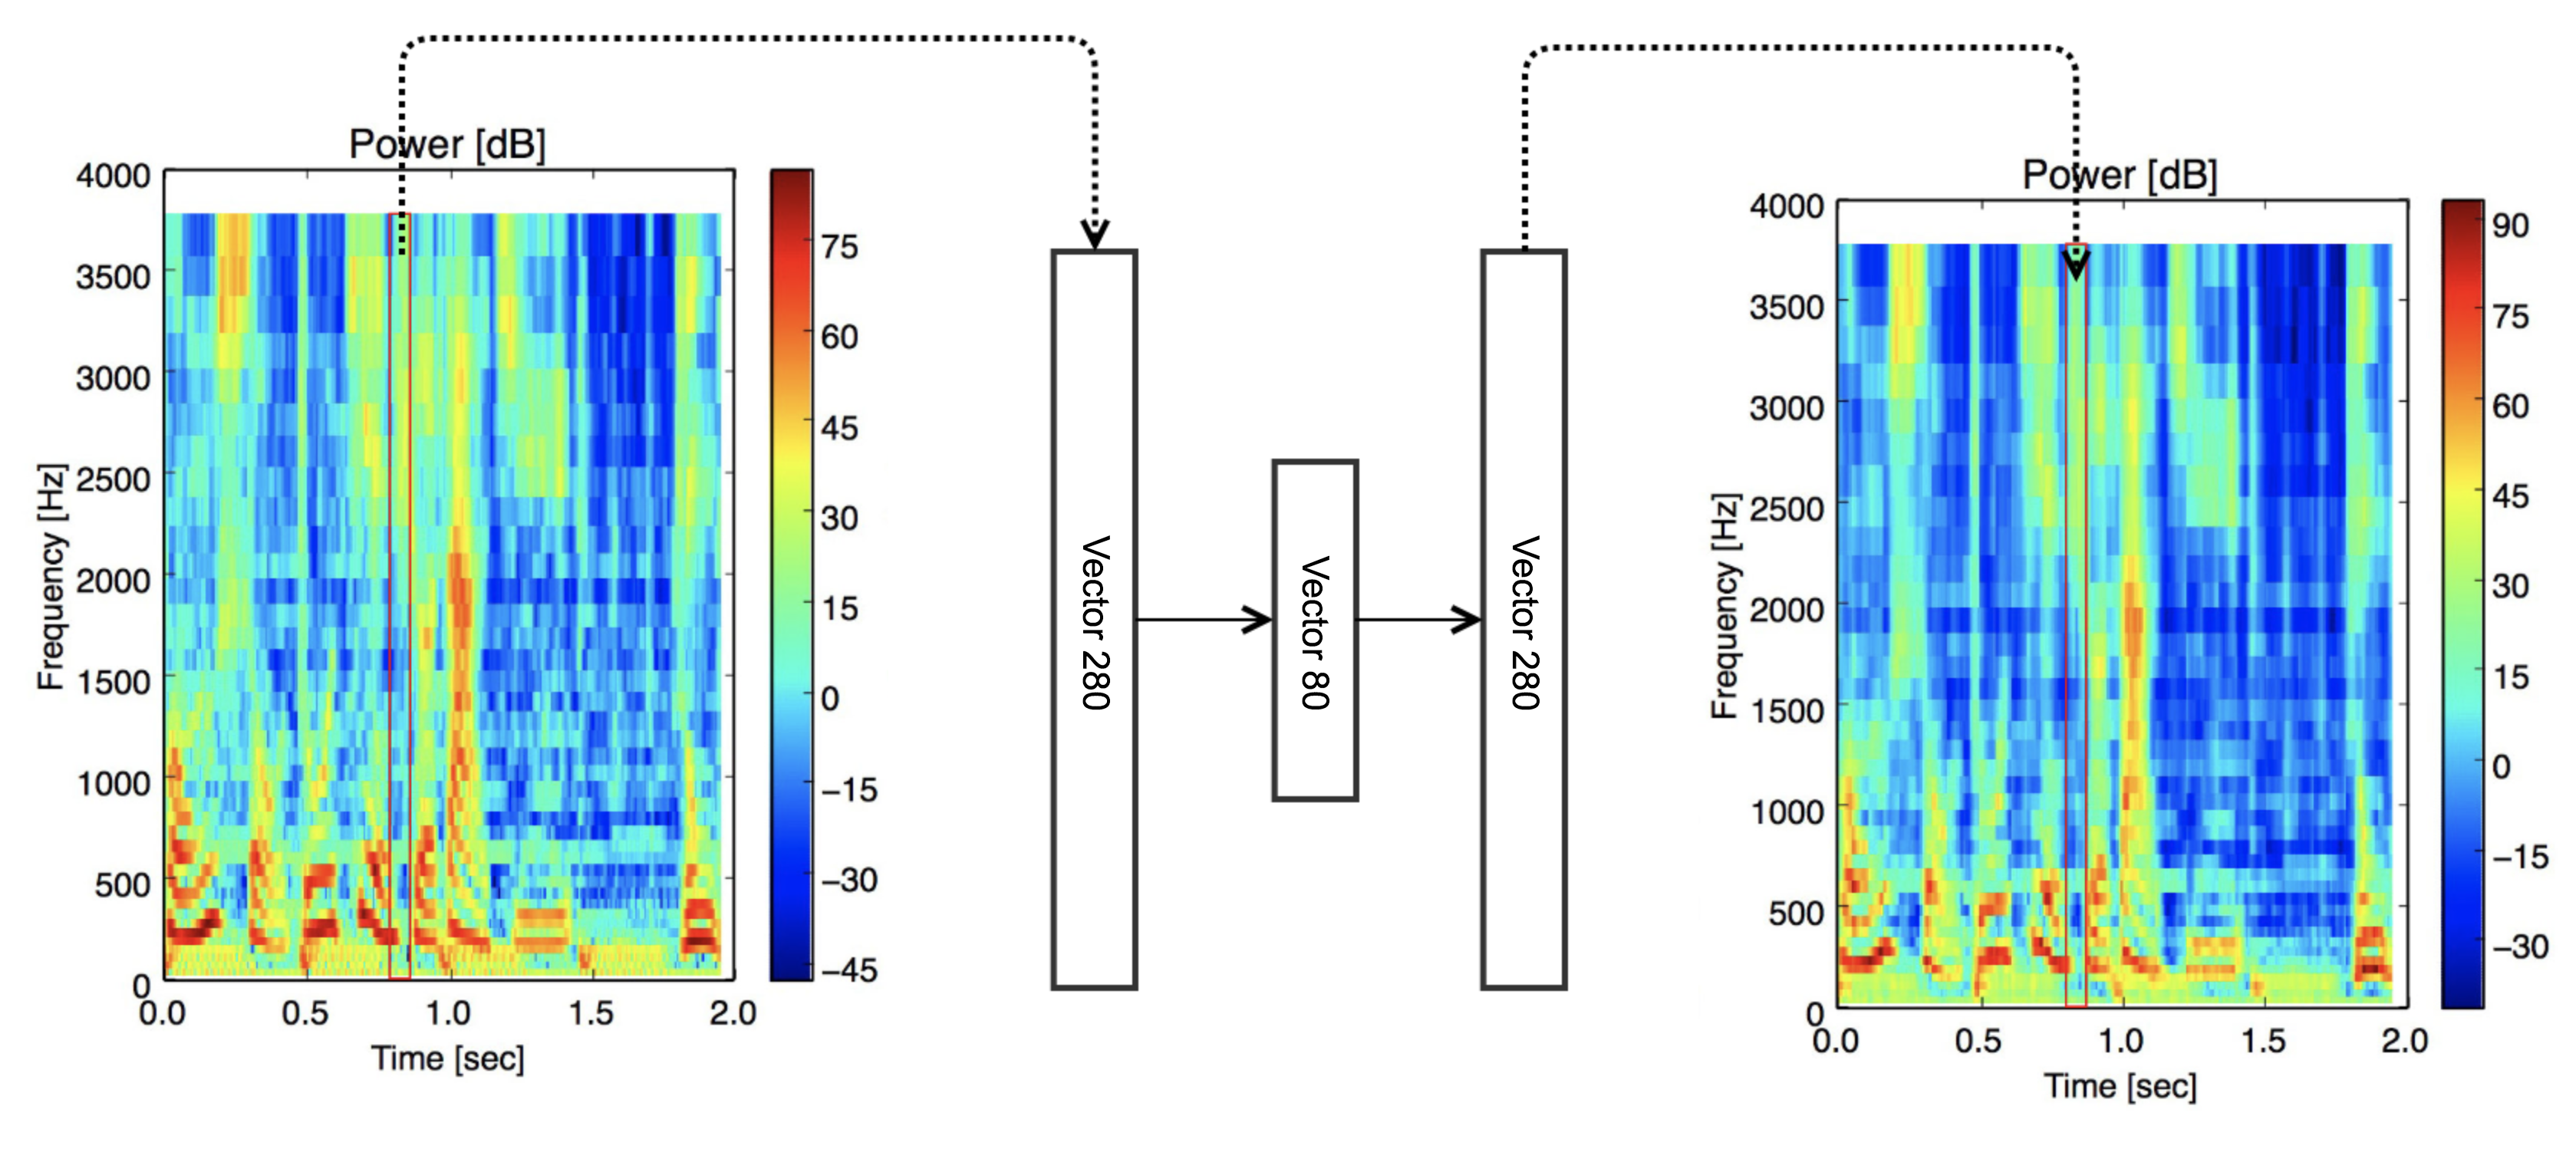
\includegraphics[width=0.8\textwidth]{autoencoder}
\caption{自编码器网络结构\label{fig:autoencoder}}
\end{figure}

自编码器网络使用tensorflow\cite{abadi2016tensorflow}实现,隐藏层激活函数使用softplus函数$\sigma(x)=ln⁡(e^x+1)$,使用质量非常高、基本未受到干扰或者噪音污染的短波语音训练自编码器,使其学习短波语音的语谱结构特征。使用总计时长约5小时的清晰短波语音进行训练,每个训练样本的语音时长为16*8=128ms,故总计样本数量为14万左右。训练的batch大小设置为256,初始学习速率0.001。
经过一段时间的训练,自编码器可以学习到清晰短波语音的语谱特征,如图~\ref{fig:ae-pure1}是一段清晰短波语音经过自编码器的输入输出结果。可以看出,尽管自编码器将输入向量的长度由输入的280压缩到了隐藏层的80,最终输入和输出的梅尔语谱图相差甚微,基本的特征都得到了保留。

\begin{figure}
\centering
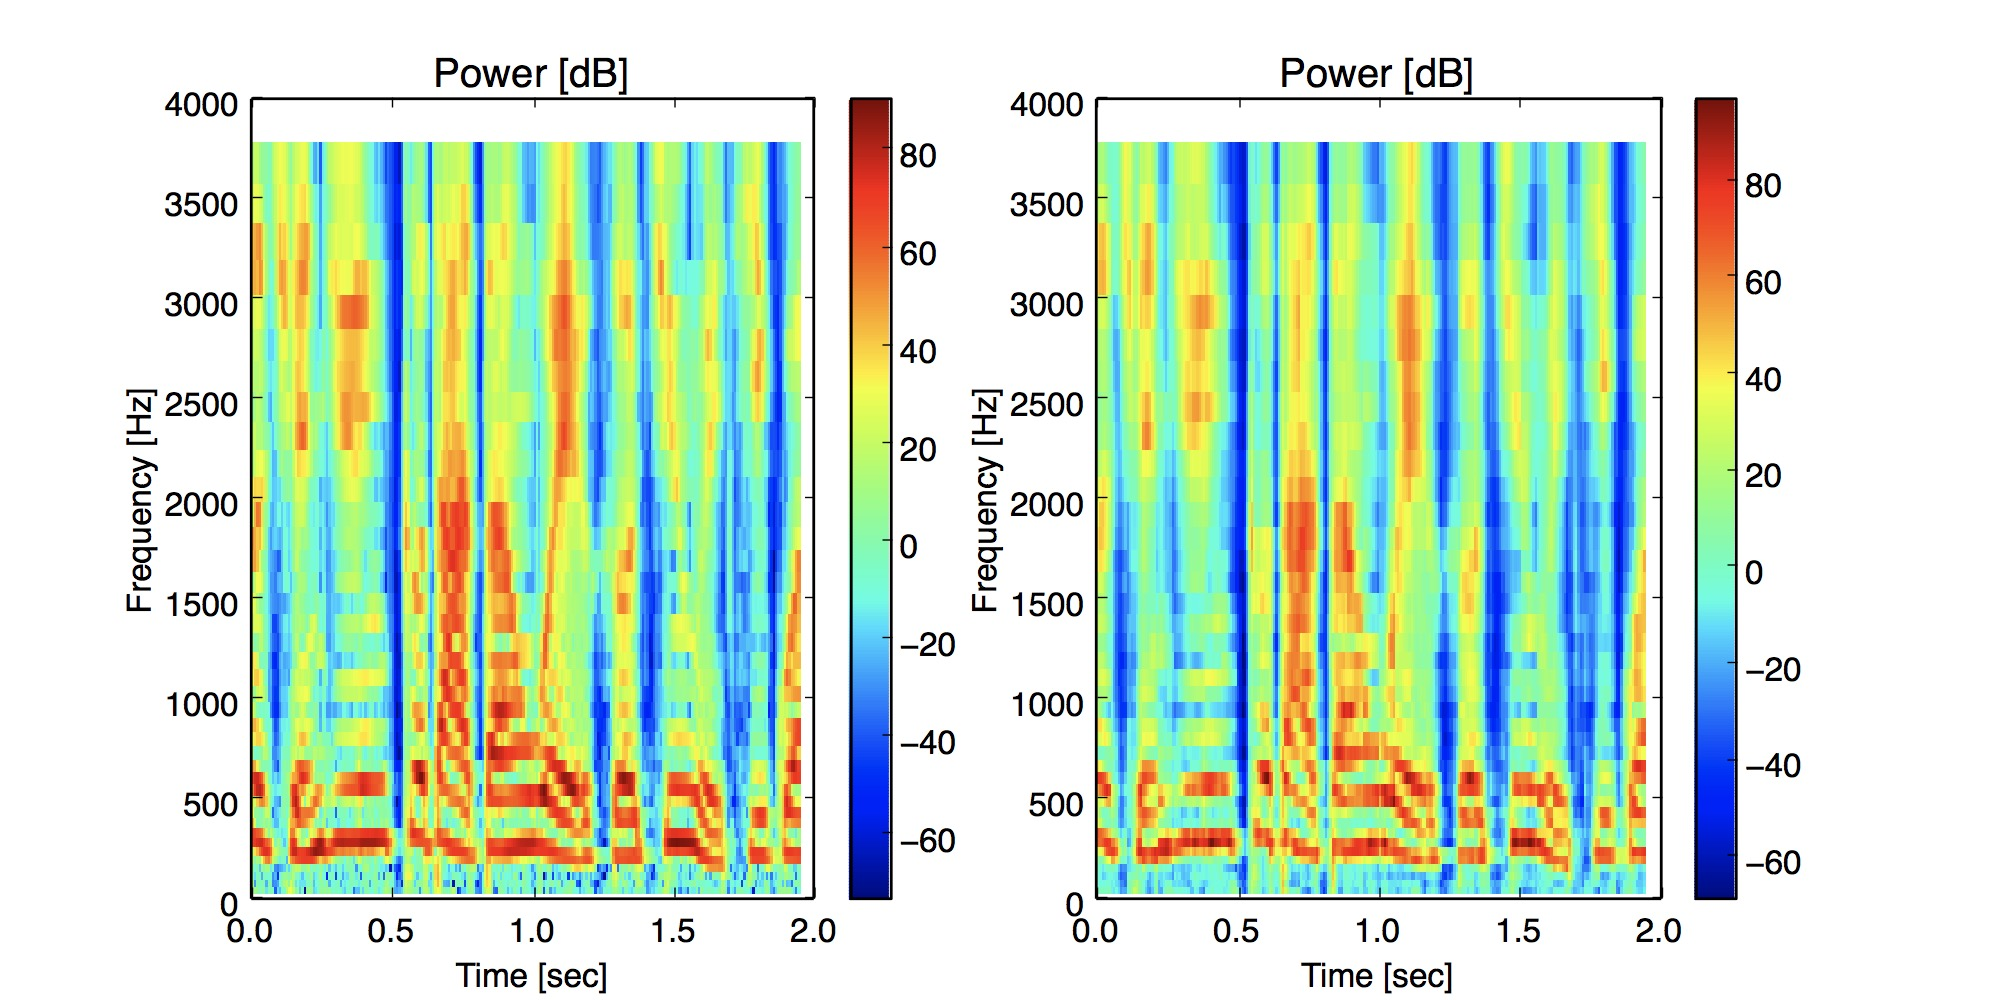
\includegraphics[width=0.8\textwidth]{ae-pure1}
\caption{自编码器输入输出语谱图(清晰语音)\label{fig:ae-pure1}}
\end{figure}
\chapter{短波语音自动选路系统}
\label{chapter:switching}

针对第~\ref{chapter:introduction}章中介绍的应用场景,即在不同地点接收多路短波语音信号,然后再根据质量进行选路的应用场景,本文基于第~\ref{chapter:algorithms}章介绍的客观质量评价算法,实现了一个不需要人工参与的短波语音自动选路系统。主要包括多路语音时间对齐算法、选路切换策略等工作,以下分别进行介绍。

\section{两路语音时间对齐}\label{section:align2}

在不同地点接收到的短波语音信号,由于短波传播路径不同,地面汇总时的传输延时不同等因素,最终收到的信号具有不同的延时。为了能够进行自动选路切换,首先需要在时间上将各路信号对齐,主要是要估计各路信号的相对延时。对齐的依据是各路信号的语音内容,这里有一个基本前提假设是各路信号的信噪比在一定水平以上,否则无法实现对齐。这样的假设是合理的,因为如果一路信号信噪比极低,完全听不见其中的语音,则不会被选路系统选作最终输出,故而也无需将它与其他各路信号对齐。

两路语音对齐算法是多路语音对齐算法的基础,这里介绍一种基于互相关的朴素算法。

设原始语音为$x(t)$,收到的两路语音信号分别为$y_1(t)$和$y_2(t)$,设两路信号延迟分别为$\delta_1$和$\delta_2$,则有以下关系:
\begin{equation}
\left\{
    \begin{array}{l}
        y_1(t) = x(t-\delta_1) + e_1(t-\delta_1) \\
        y_2(t) = x(t-\delta_2) + e_2(t-\delta_2)
    \end{array}
\right.
\end{equation}

其中$e_1$和$e_2$为两路信号传播过程中分别引入的噪音信号。

选取两路信号开头一定长时间$T>>\delta$,计算互相关函数:
\begin{equation}\label{eq:corr}
\begin{array}{c}
    C_{12}(\delta)  = \left\{
    \begin{array}{rcl}
        \int_\delta^Ty_1(t)y_2(t-\delta)dt, && {\delta \geq 0} \\
        \int_0^{T+\delta}y_1(t)y_2(t-\delta)dt, && {\delta < 0}
    \end{array}
    \right. \\
    = \left\{
    \begin{array}{rcl}
        \int_\delta^Tx(t-\delta_1)x(t-\delta_2-\delta)dt+\int_\delta^Te_1(t-\delta_1)e_2(t-\delta_2-\delta)dt, && {\delta \geq 0} \\
        \int_0^{T+\delta}x(t-\delta_1)x(t-\delta_2-\delta)dt+\int_0^{T+\delta}e_1(t-\delta_1)e_2(t-\delta_2-\delta)dt, && {\delta < 0} \\
    \end{array}
    \right.
\end{array}
\end{equation}

上式右边前一部分,在$\delta=\delta_1-\delta_2$时取得极大值,第二部分,假设噪音均为高斯白噪音,则其大小基本不随$\delta$变化。

从而当$\delta=\delta_1-\delta_2$时$C_{12}(\delta)$取得极大值,即:
\begin{equation}
\delta_1 - \delta_2 = \arg \max C_{12}(\delta)
\end{equation}
记$\delta_{12}=\delta_1-\delta_2$,为$y_1 (t)$相对于$y_2 (t)$的延迟大小,$\delta_{12}>0$表明$y_1(t)$落后于$y_2(t)$,$\delta_{12}<0$表明$y_1(t)$超前于$y_2(t)$。
通过$C_{12}(\delta)$极值点估计出$\delta_{12}$之后,即可通过截取平移获得对齐的两路语音信号$y_1^*(t)$和$y_2^*(t)$:
\begin{equation}
% \left\{
    \begin{array}{l}
        y_1^*(t)=  \left\{ 
            \begin{array}{rcl}
            y_1(t), && {\delta_{12} \geq 0} \\
            y_1(t-\delta_{12}), && {\delta_{12} < 0}
            \end{array}
        \right. \\
        \\
        y_2^*(t)= \left\{ 
            \begin{array}{rcl}
            y_2(t), && {\delta_{12} \leq 0} \\
            y_2(t+\delta_{12}), && {\delta_{12} > 0}
            \end{array}
        \right.
    \end{array}
% \right.
\end{equation}

上述对于相对延时$\delta_{12}$的估计受到以下几方面影响会存在一定误差:

\begin{enumerate}
\item 噪音污染可能不是理想白噪音,当噪音污染程度较大,即信噪比较低时会导致估计误差较大。
\item 两路语音相对延时可能较大,当延迟大小接近$T$的数量级时,截取的信号重叠部分较小,会导致估计误差较大。
\end{enumerate}

为考量这两方面因素对结果的影响,我们进行了一些测试。我们选择一段时长大约为2小时的纯净短波语音作为测试的原始语料,将其人为加上10ms的延时偏移形成两路时间不对齐的语音信号,再分别加上不同噪音等级的高斯白噪声,从而生成测试语音。随后我们在不同信噪比、不同的$T/\delta$取值情况下,随机选择1000组语音对,使用上述时间对齐算法进行对齐,统计结果的准确性。

\begin{equation}\label{eq:delay-precision}
Precision=\frac{|\delta_{before}|-|\delta_{after}|}{|\delta_{before}|}
\end{equation}

对齐结果的准确性定义为公式~\ref{eq:delay-precision},其中$\delta_{before}$和$\delta_{after}$分别为使用对齐算法之前和之后,语音的相对延时。根据该定义,$Precision$越接近$1$,代表对齐的结果越好。

\begin{figure}
\centering
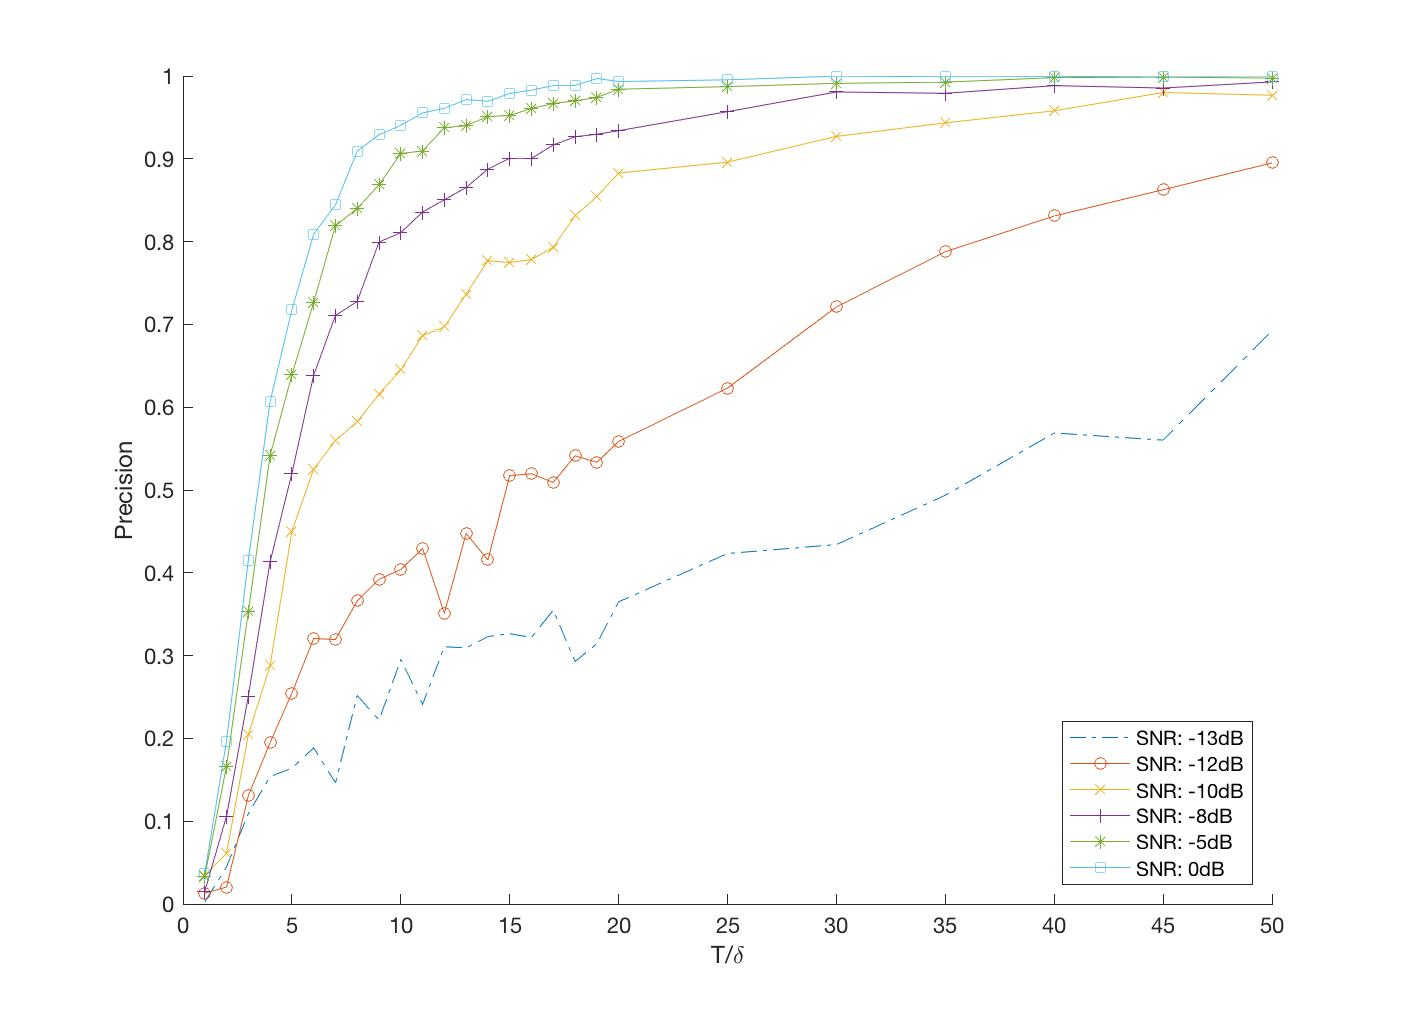
\includegraphics[width=0.8\textwidth]{test-align}
\caption{两路对齐算法测试结果\label{fig:test-align}}
\end{figure}

我们测试了信噪比为$-13dB$到$0dB$,$T/\delta$从0到50的情况,结果如图~\ref{fig:test-align}所示。图中可以看出,当信噪比低于$-12dB$时,对齐算法已经很难将语音完全对齐,这在本节开始时进行过讨论,因为信噪比过低,接收信号中的语音已经难以听清,自然难以实现时间对齐。而对齐的准确性随着$T/\delta$的增大而逐渐提高,在信噪比大于$-10dB$的情况下,$T/\delta$取到25以上就可以基本保证对齐的准确率在90\%以上,故可将$T/\delta$取为25。实际操作中,须首先估计或者测试原始相对延时$\delta$的大小,然后设定系统的$T$值大小。


\section{多路语音时间对齐} \label{section:align-multi}

在两路语音对齐算法的基础上,本节介绍一种实现多路语音时间对齐的算法。多路语音的时间对齐主要需要解决上小节算法给出的两两之间的相对延时可能存在不一致的问题,本文将该问题建模成图论问题,使用最小生成树算法进行优化选择,详述如下。

设收到有$K$路语音$(K\geq3$),分别为$y_1(t), y_2(t), ..., y_K(t)$,设指标集$I=\left\{i|i\in N^+, i\leq K\right\}$。首先使用~\ref{section:align2}节的方法我们可以估计出多路语音两两之间的相对延时$\delta_{ij}  (i,j\in I,i\neq j)$。

假设我们的估计不存在误差,且定义$\delta_{ii}=0,(i \in I)$,则
\begin{equation}\label{eq:delay-relations}
\delta_{ij}=\delta_{ik}+\delta_{jk}, \forall i,j,k \in I
\end{equation}

但是由于噪音的存在,延时的估计可能存在误差,所以两两之间的相对延时会存在不一致的情况,即公式~\ref{eq:delay-relations}并不恒成立。因而就需要从所有$K(K+1)/2$个相对延时中选取$K-1$个以确定一个统一的一致的,各路语音的相对延时。

一种最简单朴素的方法是以某一通道语音为基准,直接选取所有其他通道语音和该路语音的相对延时。例如以$y_1 (t)$为基准,选取$\delta_{1i}  (i \in I, i \neq 1)$作为统一标准确定各路语音的延时。但是这种方法得出的结果未必是最优的,如果 $y_1 (t)$ 受到的噪音污染较大,则很有可能得出的结果误差相当大。对此问题可以考虑使用后面介绍的语音质量客观评价方法来选取一路质量最优的语音作为参考基准。但是即便如此依然存在问题:如果选取的基准路语音$y_k (t)$和其他几路语音相对延时较大,而其他几路语音之间的相对延时较小,则估计的$y_k (t)$和其他几路语音的相对延时也会有较大误差,不如选取其他几路语音之间的相对延时加上$y_k (t)$和某一路语音的相对延时更好。

针对以上讨论的问题,以下介绍一种基于图论最小生成树算法来选取相对延时的方法。

我们的目标是要选取$K-1$个相对延时将所有K路语音关联起来,并使得选取的相对延时是估计准确性尽量高的。根据~\ref{section:align2}节的分析,对两路语音之间相对延时的估计的准确度可以通过互相关峰值的大小来反应,互相关的峰值越大,则准确性越高。以各路语音为节点构建一个全连通的有权无向图,各边的权值设为相连节点代表的两路语音之间互相关峰值的大小,则我们的目标可以描述为:选取$K-1$条边将$K$个节点连成一颗树,并使得$K-1$条边的权值和在所有的生成树中最大。即构造如下有权无向图
\begin{equation}
\begin{array}{l}
G(V,E), \\
V = I, \\
E = \left\{(i,j)|i, j\in I, i \neq j\right\}, \\
w(i,j)=\max⁡ \left\{ C_{ij}(\delta) \right\}
\end{array}
\end{equation}

问题即转化成求解图$G$的最大生成树,最大生成树和最小生成树可互相转化,直接对所有边权重求相反数即可。最小生成树是图论中非常经典的一个问题,有诸多相关的算法研究~\cite{bazlamaccci2001minimum}。

求解最小生成树问题的经典算法有Boruvka算法、Prim算法和Kruskal算法等。Boruvka算法是最古老的最小生成树算法,时间复杂度为$O(|E|log|V|)$;Prim算法和Kruskal算法是最常用和广为人知的两种最小生成树算法,时间复杂度分别为$O(|E|+|V|log|V|)$和$O(|E|log|E|)$。Yao~\cite{yao19750}在Boruvka算法基础上改进提出了一种更快速的算法,时间复杂度为$O(|E|loglog|V|)$。而Karger等人~\cite{karger1995randomized}提出的线性时间算法是目前最快的最小生成树算法。我们使用经典的Prim算法,如算法~\ref{alg:prim}所示。

\begin{algorithm}
    \caption{求解最小生成树的Prim算法}
    \label{alg:prim}
\begin{algorithmic}[1]
\INPUT
    \Statex 一个加权连通图,$G(V, E)$,其中V为顶点集合,E为边集合
\OUTPUT
    \Statex 最小生成树$T(V_T, E_T)$,其中$V_T = V$是最小生成树的顶点集合,$E_T \in E$是最小生成树的边集合
\State 初始化$V_T = {x}$,其中$x$为集合$V$中的任一顶点,$E_T = {}$,为空
\State $i=l-1, j=r+1, k=l$
\While { $V_T \neq V$; }
    \State 在集合$E$中选取权值最小的边$<u, v>$,其中$u \in V_T, v \not\in V_T$;
    \State 将边$<u, v>$加入集合$E_T$,顶点$v$加入集合$V_T$
\EndWhile
\end{algorithmic}
\end{algorithm}

得到最大生成树后,生成树上对应的边即代表应该选取的相对延迟估计,在这$K-1$个相对延迟的基础上,利用式x.x.x即可求出各路信号相对$y_1 (t)$的延迟$\delta_{i1},(i \in I)$,其中$\delta_{11}=0$。随后对各路信号进行对齐和平移,得到时间对齐后的信号:
\begin{equation}
y_i^* (t)=y_i (t+\delta_{i1}-\min_{j\in I}\delta_{j1})
\end{equation}

类似两路对齐算法,我们对多路对齐算法也进行了相应的测试。我们生成了具有不同延时的5路语音信号,并给他们添加不同能量大小的高斯噪音以测试不同信噪比的情况。生成的5路语音延时如表~\ref{tab:delays}所示。为了与两路语音对齐做比较,我们特意设置通路1和通路5之间的相对延时为10ms,与两路语音对齐测试一致。

\begin{table}
\centering
\caption{测试用各路语音延时}
\label{tab:delays}
\begin{tabular}{ccc}
\toprule[1.5pt]
通路编号 & 相对通路1的延时$\delta_{i1}$ \\ \midrule[1pt]
1 & 0ms \\
2 & -3ms \\
3 & 2ms \\
4 & 6ms \\
5 & 10ms \\
\end{tabular}
\end{table}

\begin{figure}
\centering
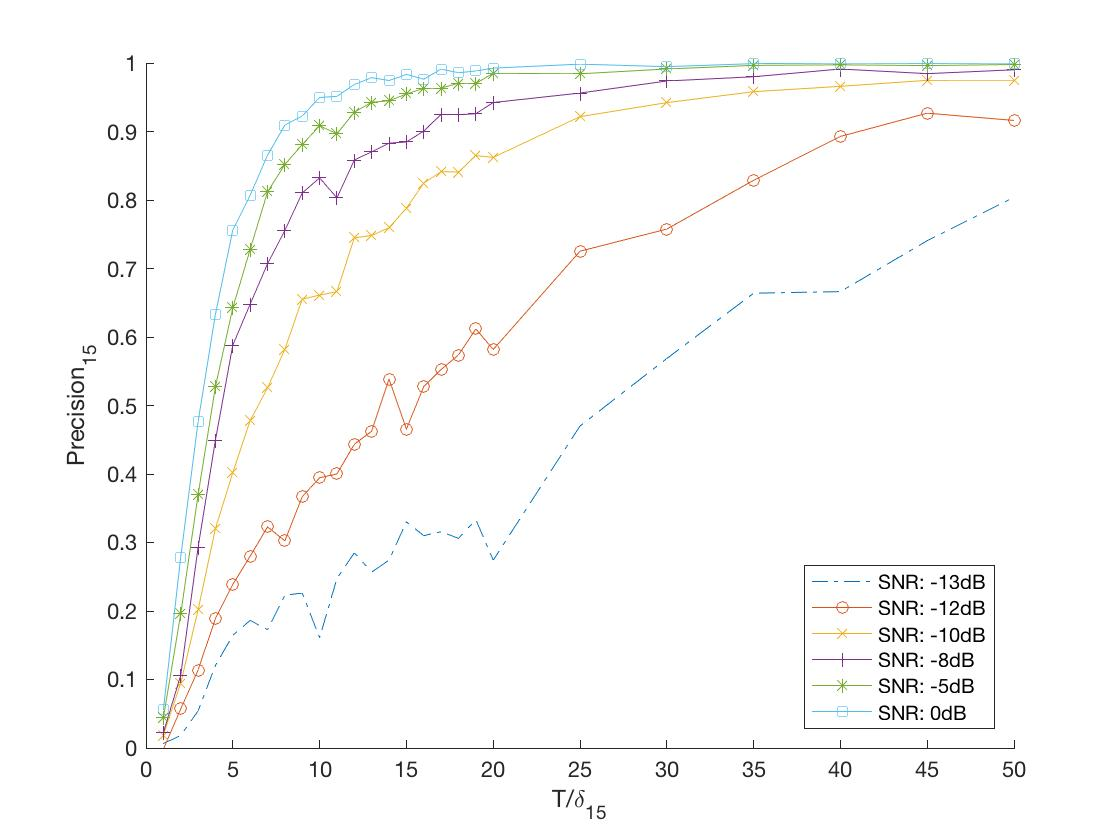
\includegraphics[width=0.8\textwidth]{test-align-multi}
\caption{多路对齐算法测试结果\label{fig:test-align-multi}}
\end{figure}

\begin{figure}
\centering
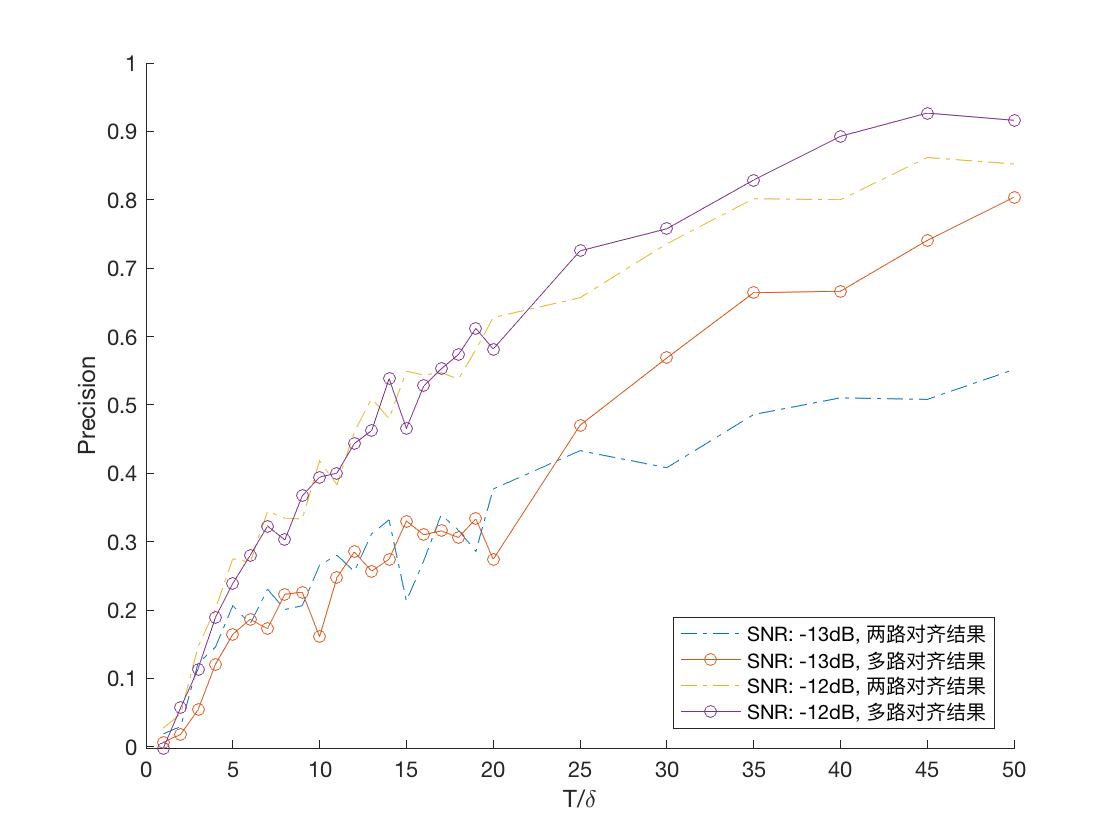
\includegraphics[width=0.8\textwidth]{compare-align}
\caption{多路对齐算法与两路对齐算法比较\label{fig:compare-align}}
\end{figure}

我们测试信噪比从$-13dB$到$0dB$,$T/\delta_{15}$从0到50的情况,分析多路对齐算法对通路1和通路5对齐结果的准确性,每组实验进行1000次取平均,结果如图~\ref{fig:test-align-multi}所示。可以看到和两路语音对齐一样,对于信噪比在$12dB$以上的情况,$T/\delta_{15} > 25$就可以基本保证90\%以上的对齐准确率。

而且,由于我们使用最小生成树策略在5路信号之间选择了更可信的4对相对延时时间构建了整体的相对延时,使得在低信噪比的情况下,多路对齐的结果比直接两路对齐的效果更好。如图~\ref{fig:compare-align}所示,我们比较了信噪比为$-13dB$和$-12dB$情况下,直接两路对齐和多路对齐的结果,其中多路对齐选择1路和5路的对齐准确率,这两路信号的相对延时为10ms,与两路对齐测试中一致。由于利用了另外三路信号的信息,可以看到多路对齐的结果要明显由于直接两路对齐的结果,可见我们多路对齐算法的策略起到了很好的作用。

\section{实时多路对齐算法} \label{section:realtime-align}

实际应用中,往往要求对多路语音信号进行实时处理。在~\ref{section:align-multi}节基础上,本节介绍一种对于多路语音信号流进行实时对齐的算法。

在实时的信号处理中,缓冲队列是非常常见的结构,本文采用多级缓冲队列的形式实现实时的多路语音对齐。第一级缓冲队列接收各路信号的输入,对于每一路语音使用一个缓冲队列存储最近一段时间的信号,新到达的信号从队尾加入队列,通过对齐算法计算各路语音的相对延时从而控制各路信号出队列的时间,也即进入第二级缓冲队列的时间,使得第二级缓冲队列中的各路信号是时间对齐的,可用于后续的计算和处理。

\begin{figure}
\centering
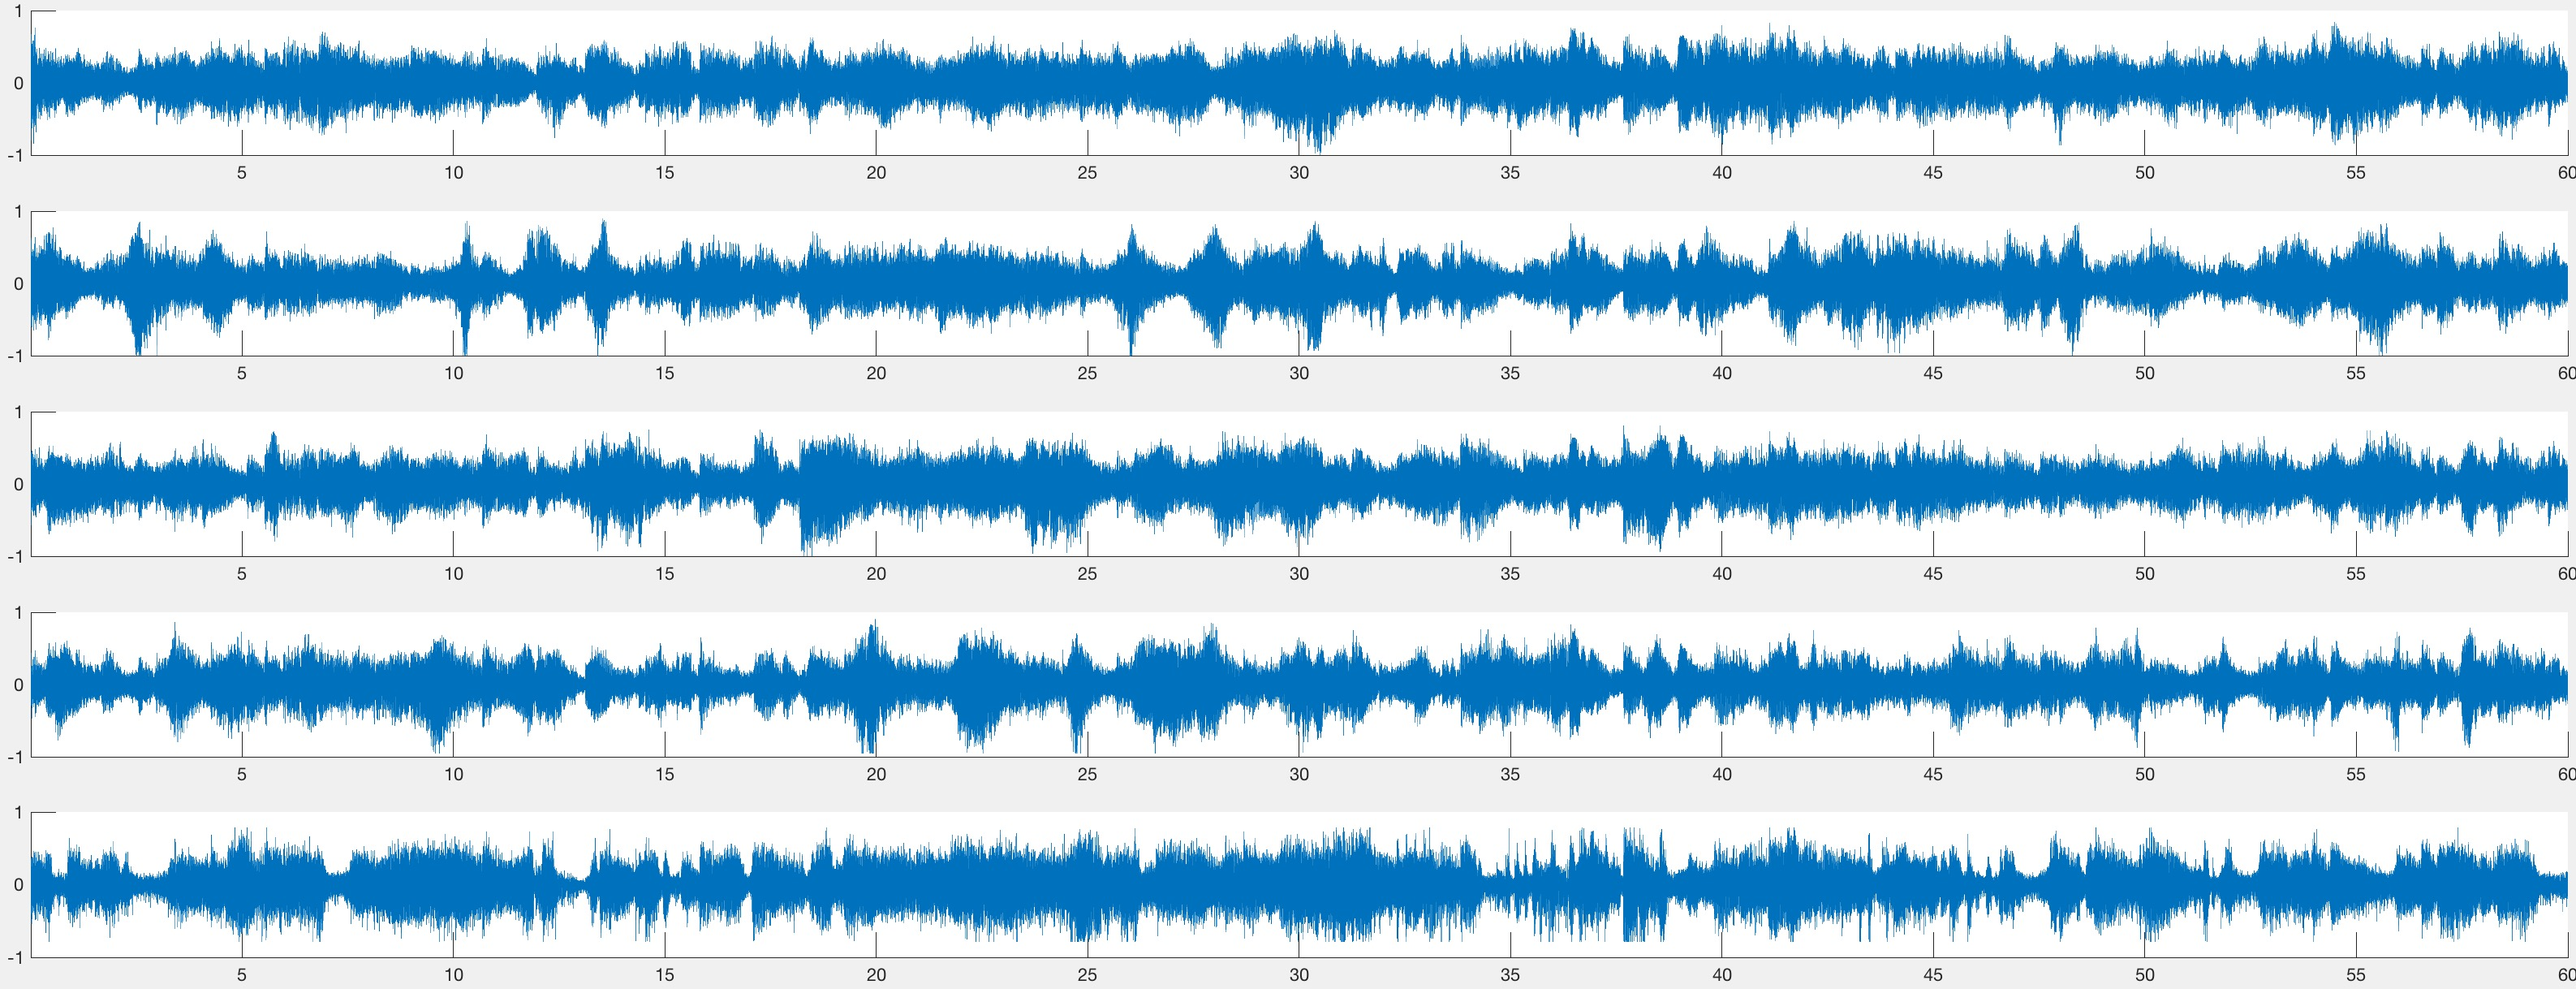
\includegraphics[width=0.8\textwidth]{multi-align}
\caption{实时对齐算法示意\label{fig:multi-align}}
\end{figure}

为便于理解,可以想象语音信号是固定的队列,而一级缓冲队列则是在移动的队首和队尾指针。如图~\ref{fig:multi-align}所示,将语音信号想象成一个无限长的队列,然后有一个队首指针和队尾指针,两个指针之间的部分即使算法目前实际缓存的语音信号部分。由于随着时间推移不断接收到新的信号,所以队尾指针会随着时间以固定速率后移,而队首指针则是在算法控制下后移以调整延时,最终稳定时,队首和队尾的指针均匀速后移,各路信号缓存的长度不同,队首指针处的信号是时间上对齐的,各个一级缓冲队列的队列长度则因为信号延时不同而不同。

算法一开始首先保证各路信号均缓存了时间长度为的数据。随后使用~\ref{section:align-multi}节中的算法可以得出各路信号相对第一路信号的延迟$\delta_{i1}, i \in I$,可能为负值,找到最大的延时,记为$\delta_{k1} = \max \delta_{i1}$,则为了保证队首指针时间对齐,第$i$路信号的队首指针应暂停$\delta_{k1}-\delta_{i1}$时间不移动。这相当于第$i$路信号的延迟增加了$\delta_{k1}-\delta_{i1}$,于是各路信号的队首均对齐到了路信号。之后每0.1秒执行一次上述步骤进行对齐调整。

进一步,为了保证算法的稳定性,降低执行过程中对于相对延时突发的错误估计造成的影响,可以设置一个调整步长$0<\alpha<1$,各路队首指针暂停时间修改为$\alpha(\delta_{k1}-\delta_{i1})$。$\alpha$越大则越快收敛到对齐状态,但是越不稳定;相反越小则收敛速度越慢,但是越稳定。可以根据情况设定$\alpha$的取值。

另外,此方法永远在增加信号的延迟,会导致合路信号的延迟越来越大,可以做如下改进:每次对齐调整完成后,如果最短的缓存队列长度为超过了$T$,则所有路信号的队首指针同时向后调整使得最短的缓存队列长度缩短为$T$。这样,合路信号的延迟永远为延迟最大的一路信号的延迟加上$T$。

最终的算法流程参见算法~\ref{alg:live-align}。

\begin{algorithm}
    \caption{多路语音实时对齐算法}
    \label{alg:live-align}
\begin{algorithmic}[1]
\INPUT
    \Statex 实时推送的多路语音信号
\OUTPUT
    \Statex 实时输出时间对齐的多路语音信号
\State 初始化多路语音的缓冲队列$Q_i, i\in I$,接收到的各路语音会定时进入各个队列的队尾
\State 等待各路语音的缓冲队列长度超过$T$
\State 初始化各路语音信号的时间调节变量$D_i$全部为0
\While { true; }
    \For { $i \in I$ }
        \If { $D_i = 0$ }
            \State 语音缓冲队列$Q_i$队首出队列并且输出
        \Else
            \State $Q_i = Q_i - 1$
        \EndIf
    \EndFor
    \If { 所有的$Q_i$的长度均超过$T$ }
        \State 所有语音缓冲队列队首出队列并且输出
    \EndIf
    \If { 距上一次计算相对延迟已达到0.1秒或尚未计算相对延迟 }
        \State 使用~\ref{section:align-multi}节描述的算法计算各路语音的相对延时$\delta_{ij}$
        \State 在$\delta_{i1}$中找到最大值$\delta_{k1}$
        \For { $i \in I$ }
            \State $D_i = D_i + \alpha(\delta_{k1}-\delta_{ki})$
        \EndFor
    \EndIf
    \State 休眠一个采样时间
\EndWhile
\end{algorithmic}
\end{algorithm}

\section{选路策略及系统设计}

本节介绍短波语音信号的选路策略以及选路系统的设计。由于各路信号的强度和背景噪音不同,如果直接对各段时间内的信号,总是切换到质量评分最高的一路信号,可能出现信号切换过于频繁,导致听起来连贯的问题,反而影响合路信号的质量。以下几项策略保证了合路信号在选择尽量优质量的语音通路的同时,提高合路语音的自然度。

\begin{enumerate}
    \item 需要对各路语音的功率进行归一化处理,可以使用各路语音的均值功率作为参考,将各路语音信号放大或缩小从而统一功率。
    \item 为防止意外状况导致的错误评分带来的抖动,对各路语音的实时评分经过一个低通滤波作为选路参考的分值。
    \item 为了避免过度频繁的切换语音通路,设定一个适当大小的阈值,只有当新的最优通路的评分超过当前选择通路的评分达到一定阈值,才切换至新的最优通路。否则依然保持原来选择的通路。 
    \item 在通路切换时,采用线性渐变的过度来平滑切换的过程。
\end{enumerate}

\begin{figure}
\centering
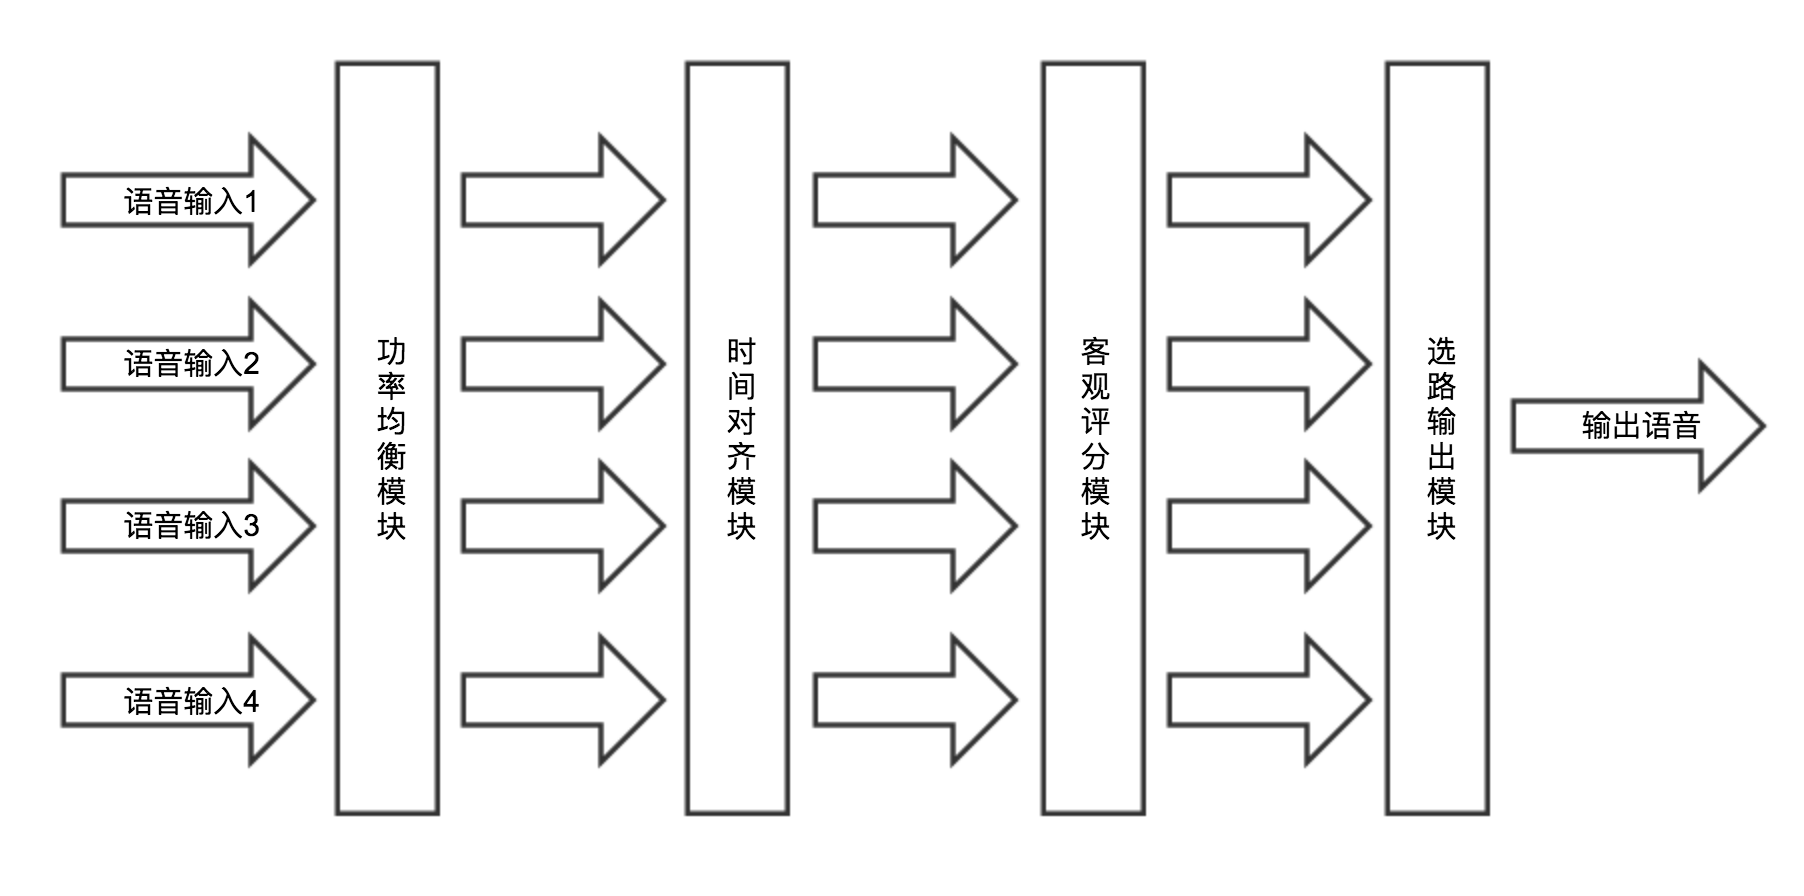
\includegraphics[width=0.8\textwidth]{switching-sys}
\caption{选路系统结构\label{fig:switching-sys}}
\end{figure}

如图~\ref{fig:switching-sys}所示,选路系统分为“功率均衡模块”、“时间对齐模块”、“客观评分模块”、“选路输出模块”这四个模块,分别实现上述几项策略。

功率均衡模块负责均衡各路语音信号的功率,具体步骤如下:统计每一路输入最近1s时间内的信号功率$P_i, i \in I$,将其经过一个低通滤波器,得到滤波后的平均信号功率$\bar{P_i}$,据此可利用式~\ref{eq:power-gain}计算各路的信号增益$Gain_i$,各路信号分别乘上对应增益实现各路信号的功率均衡。
\begin{equation}\label{eq:power-gain}
Gain_i = \sqrt{\frac {K\bar{P_i}} {\sum_{k \in I}{\bar{P_k}}} }
\end{equation}

时间对齐模块负责各路语音信号的时间对齐,使用~\ref{section:realtime-align}节介绍的算法实现。

客观评分模块对每一路最近1s内的信号使用第~\ref{chapter:algorithms}章介绍的算法进行客观评分,然后再通过低通滤波器得到去除抖动后的质量评分$\bar{S_i}, i \in I$。

选路输出模块负责选路切换,设定切换阈值$T_{switch}$,若当前输出为$i$路语音,切换到第$j$路语音的条件为:
\begin{equation}
\begin{array}{l}
\bar{S_j} = \max\limits_{k \in I} \bar{S_k} \\
\bar{S_j} - \bar{S_i} > T_{switch}
\end{array}
\end{equation}

在发生切换时,切换模块自动完成线性平滑过度,设定切换时长为$\Delta$,则切换阶段输出语音可表示为:
\begin{equation}
y_{out}(t) = \frac{ty_j(t)+(\Delta-t)y_i(t)}{\Delta}
\end{equation}

\section{小结}

本章主要介绍了短波语音自动选路系统。首先介绍了关键的多路语音时间对齐算法,包括基于互相关的两路语音时间对齐算法、基于最小生成树的多路语音时间对齐算法以及使用缓冲队列实现的实时对齐算法。然后介绍了自动选路系统的设计,包括功率均衡模块、时间对齐模块、客观评分模块和选路切换模块。该系统通过自动客观评分切换选择质量最优的一路信号,并且利用时间对齐算法、功率均衡策略、平滑滤波以及阈值切换策略等保证了输出语音的连贯性。

\chapter{短波语音主观评价在线辅助系统} \label{chapter:web}


客观评分算法的目标是希望能够尽量逼近人的主观感受,为了验证本文客观评分算法的效果,需要获得短波语音的主观平均意见分,即MOS(Mean Opinion Score)。由于低信噪比的短波信道语音质量相对较低,且浮动范围大,志愿者在不知道语音整体质量范围的情况下直接打分,结果会有失偏颇。所以本文先对随机选取的短波语音按照主观比较结果进行排序,确定短波语音的整体质量范围,从而确定评分的参考标准。

为方便短波语音的主观排序和MOS分生成,本文实现了一个在线辅助系统,志愿者可以在线试听、比较、评价短波语音,可用于组织短波语音的主观评价实验。

\section{系统功能介绍}

短波语音主观评价辅助系统主要具有两大功能,一是通过和志愿者的交互,对一系列短波语音按照主观感受质量进行排序;二是通过搜集志愿者对短波语音的评分,计算各个短波语音的平均主观意见分。

\begin{figure}
\centering
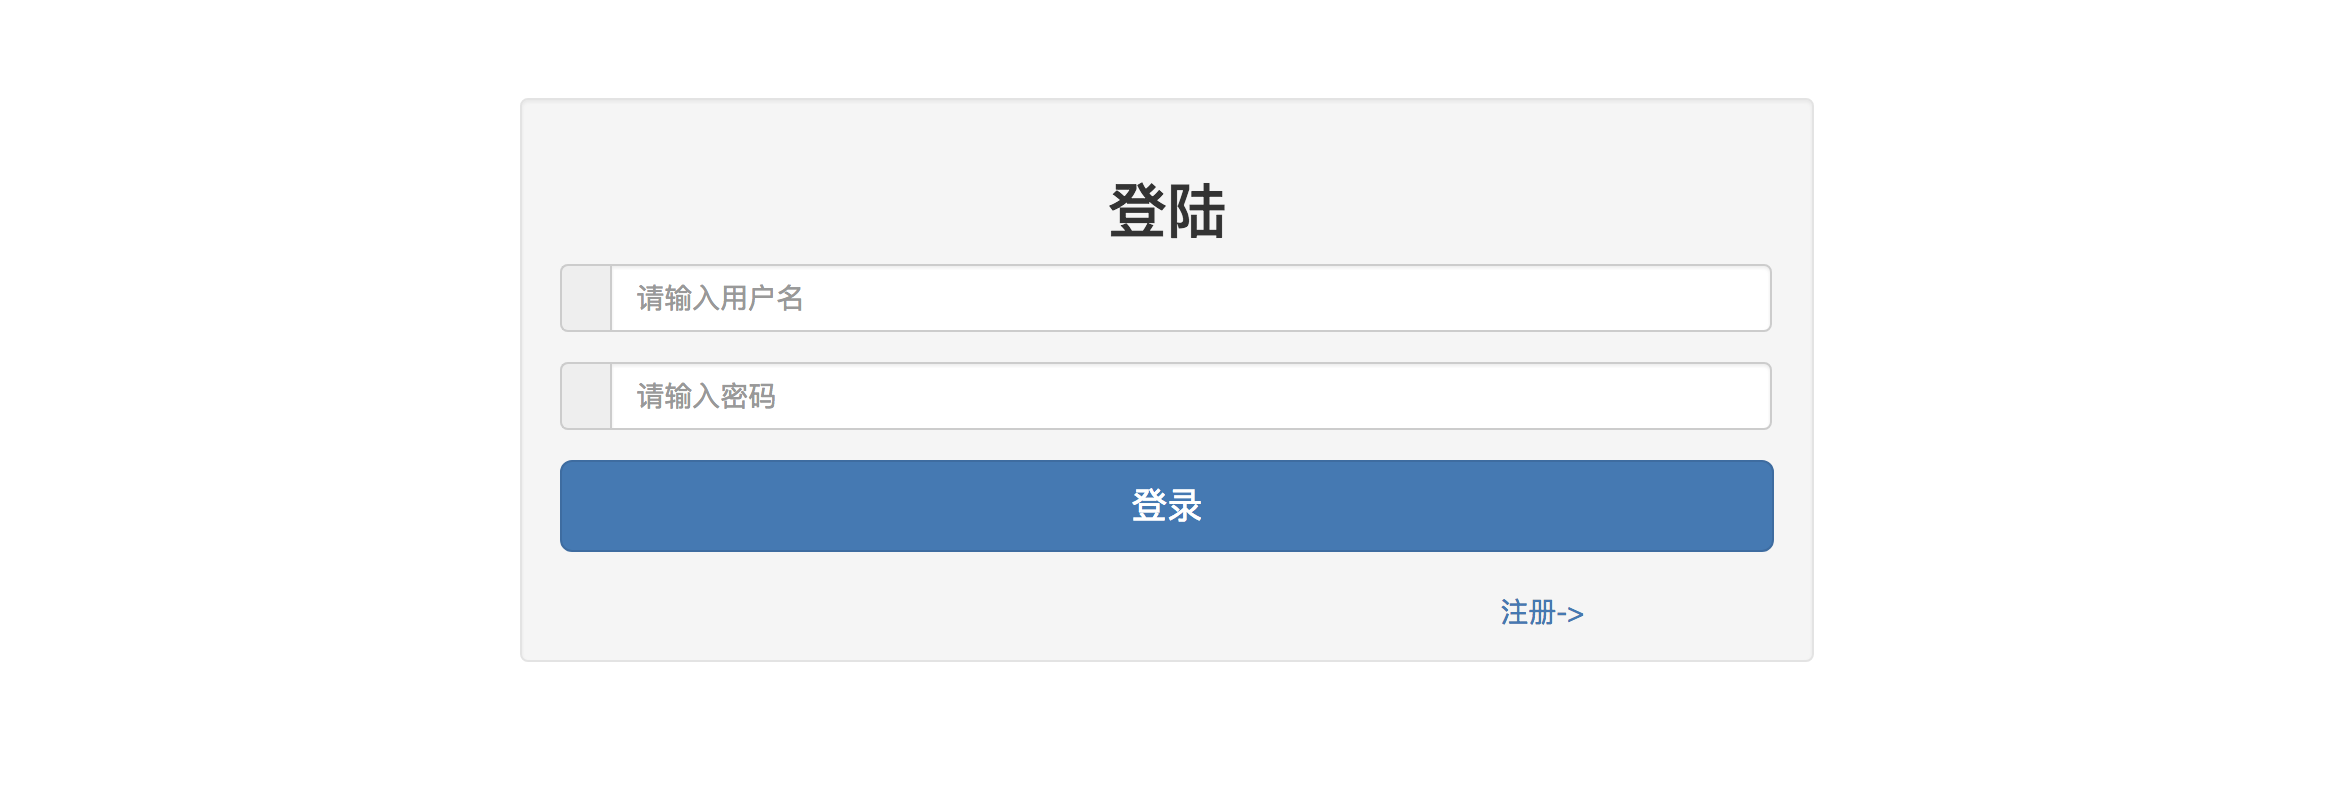
\includegraphics[width=0.8\textwidth]{web-login}
\caption{在线辅助系统的登陆界面\label{fig:web-login}}
\end{figure}

该辅助系统分为管理端和志愿者端,如图~\ref{fig:web-login}为系统登录界面,使用管理员账户登录可进入管理端,否则进入志愿者端。点击“注册”可以进行志愿者账号注册。

\begin{figure}
\centering
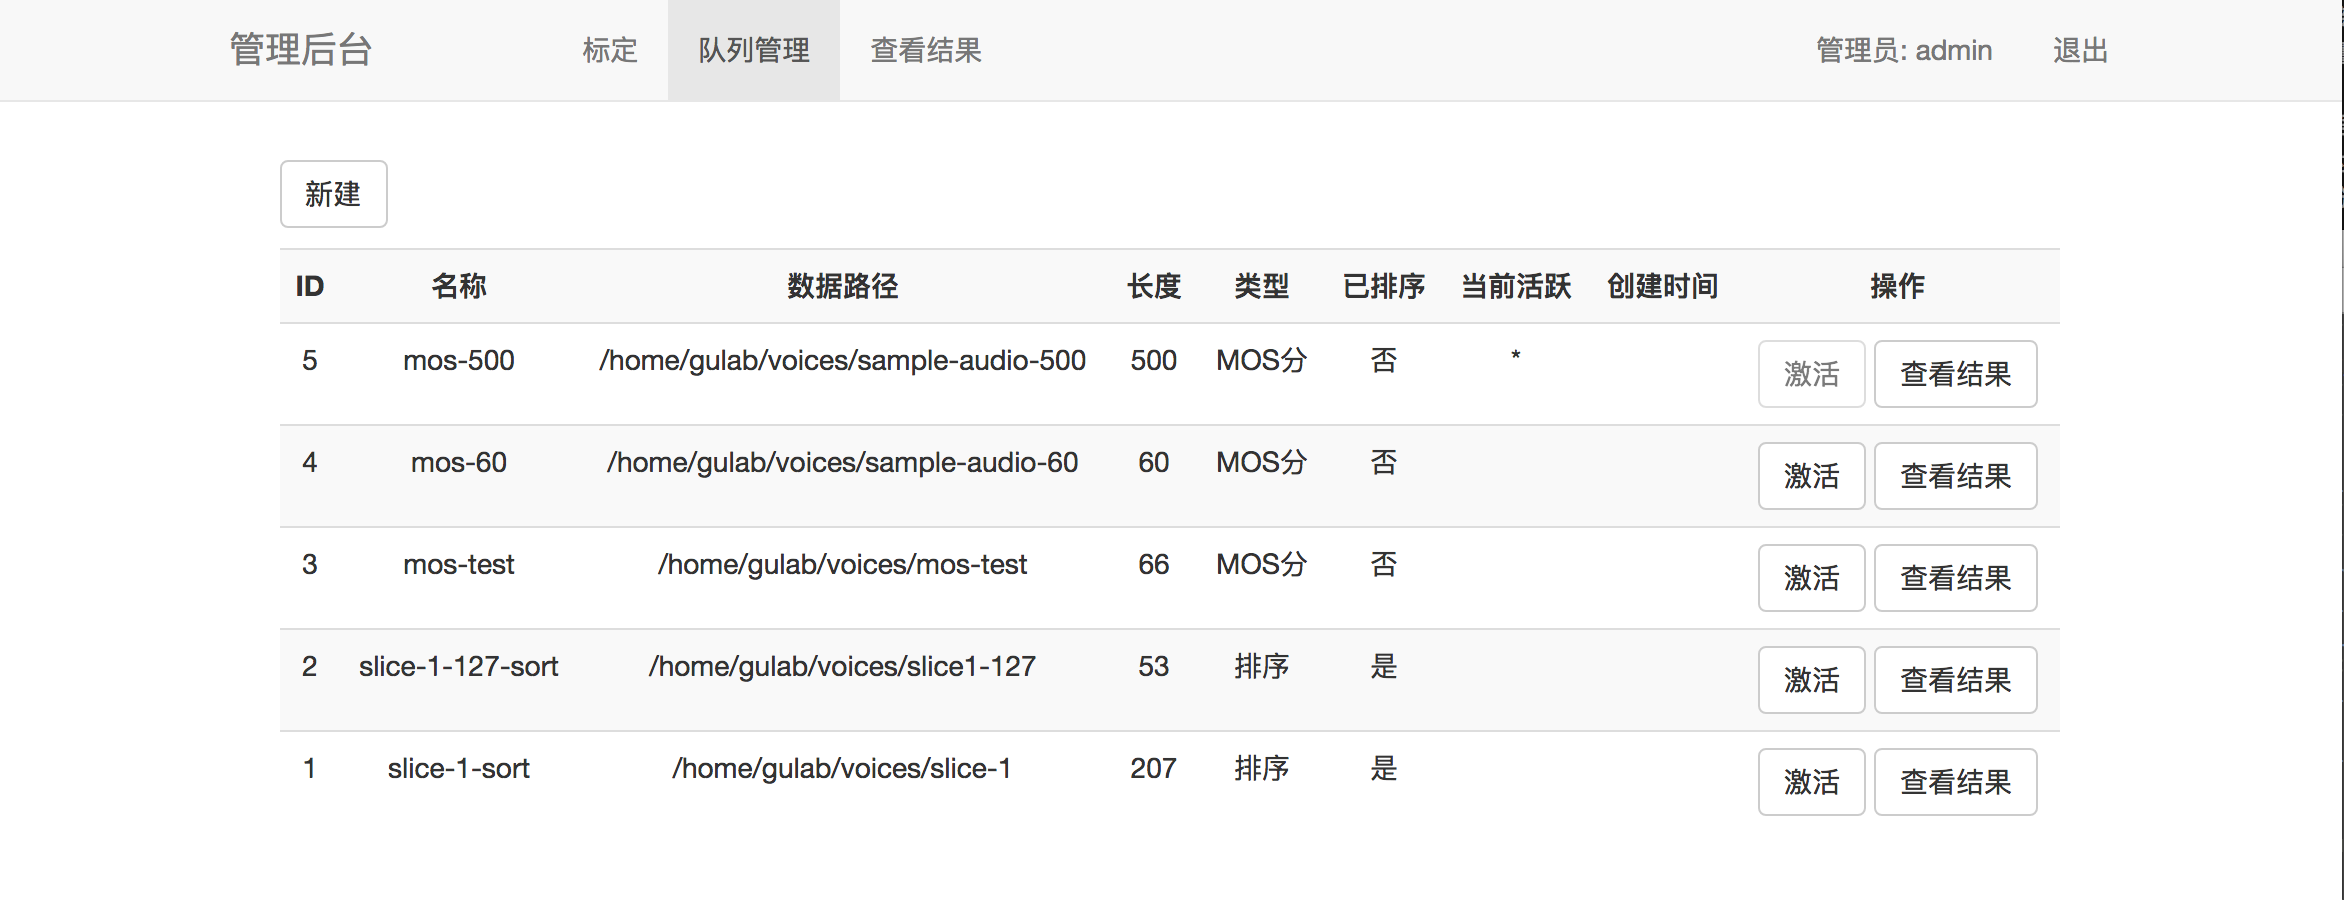
\includegraphics[width=0.8\textwidth]{web-queues}
\caption{在线辅助系统的队列管理界面\label{fig:web-queues}}
\end{figure}

\begin{figure}
\centering
\subcaptionbox{排序结果\label{fig:web-sort}}{
    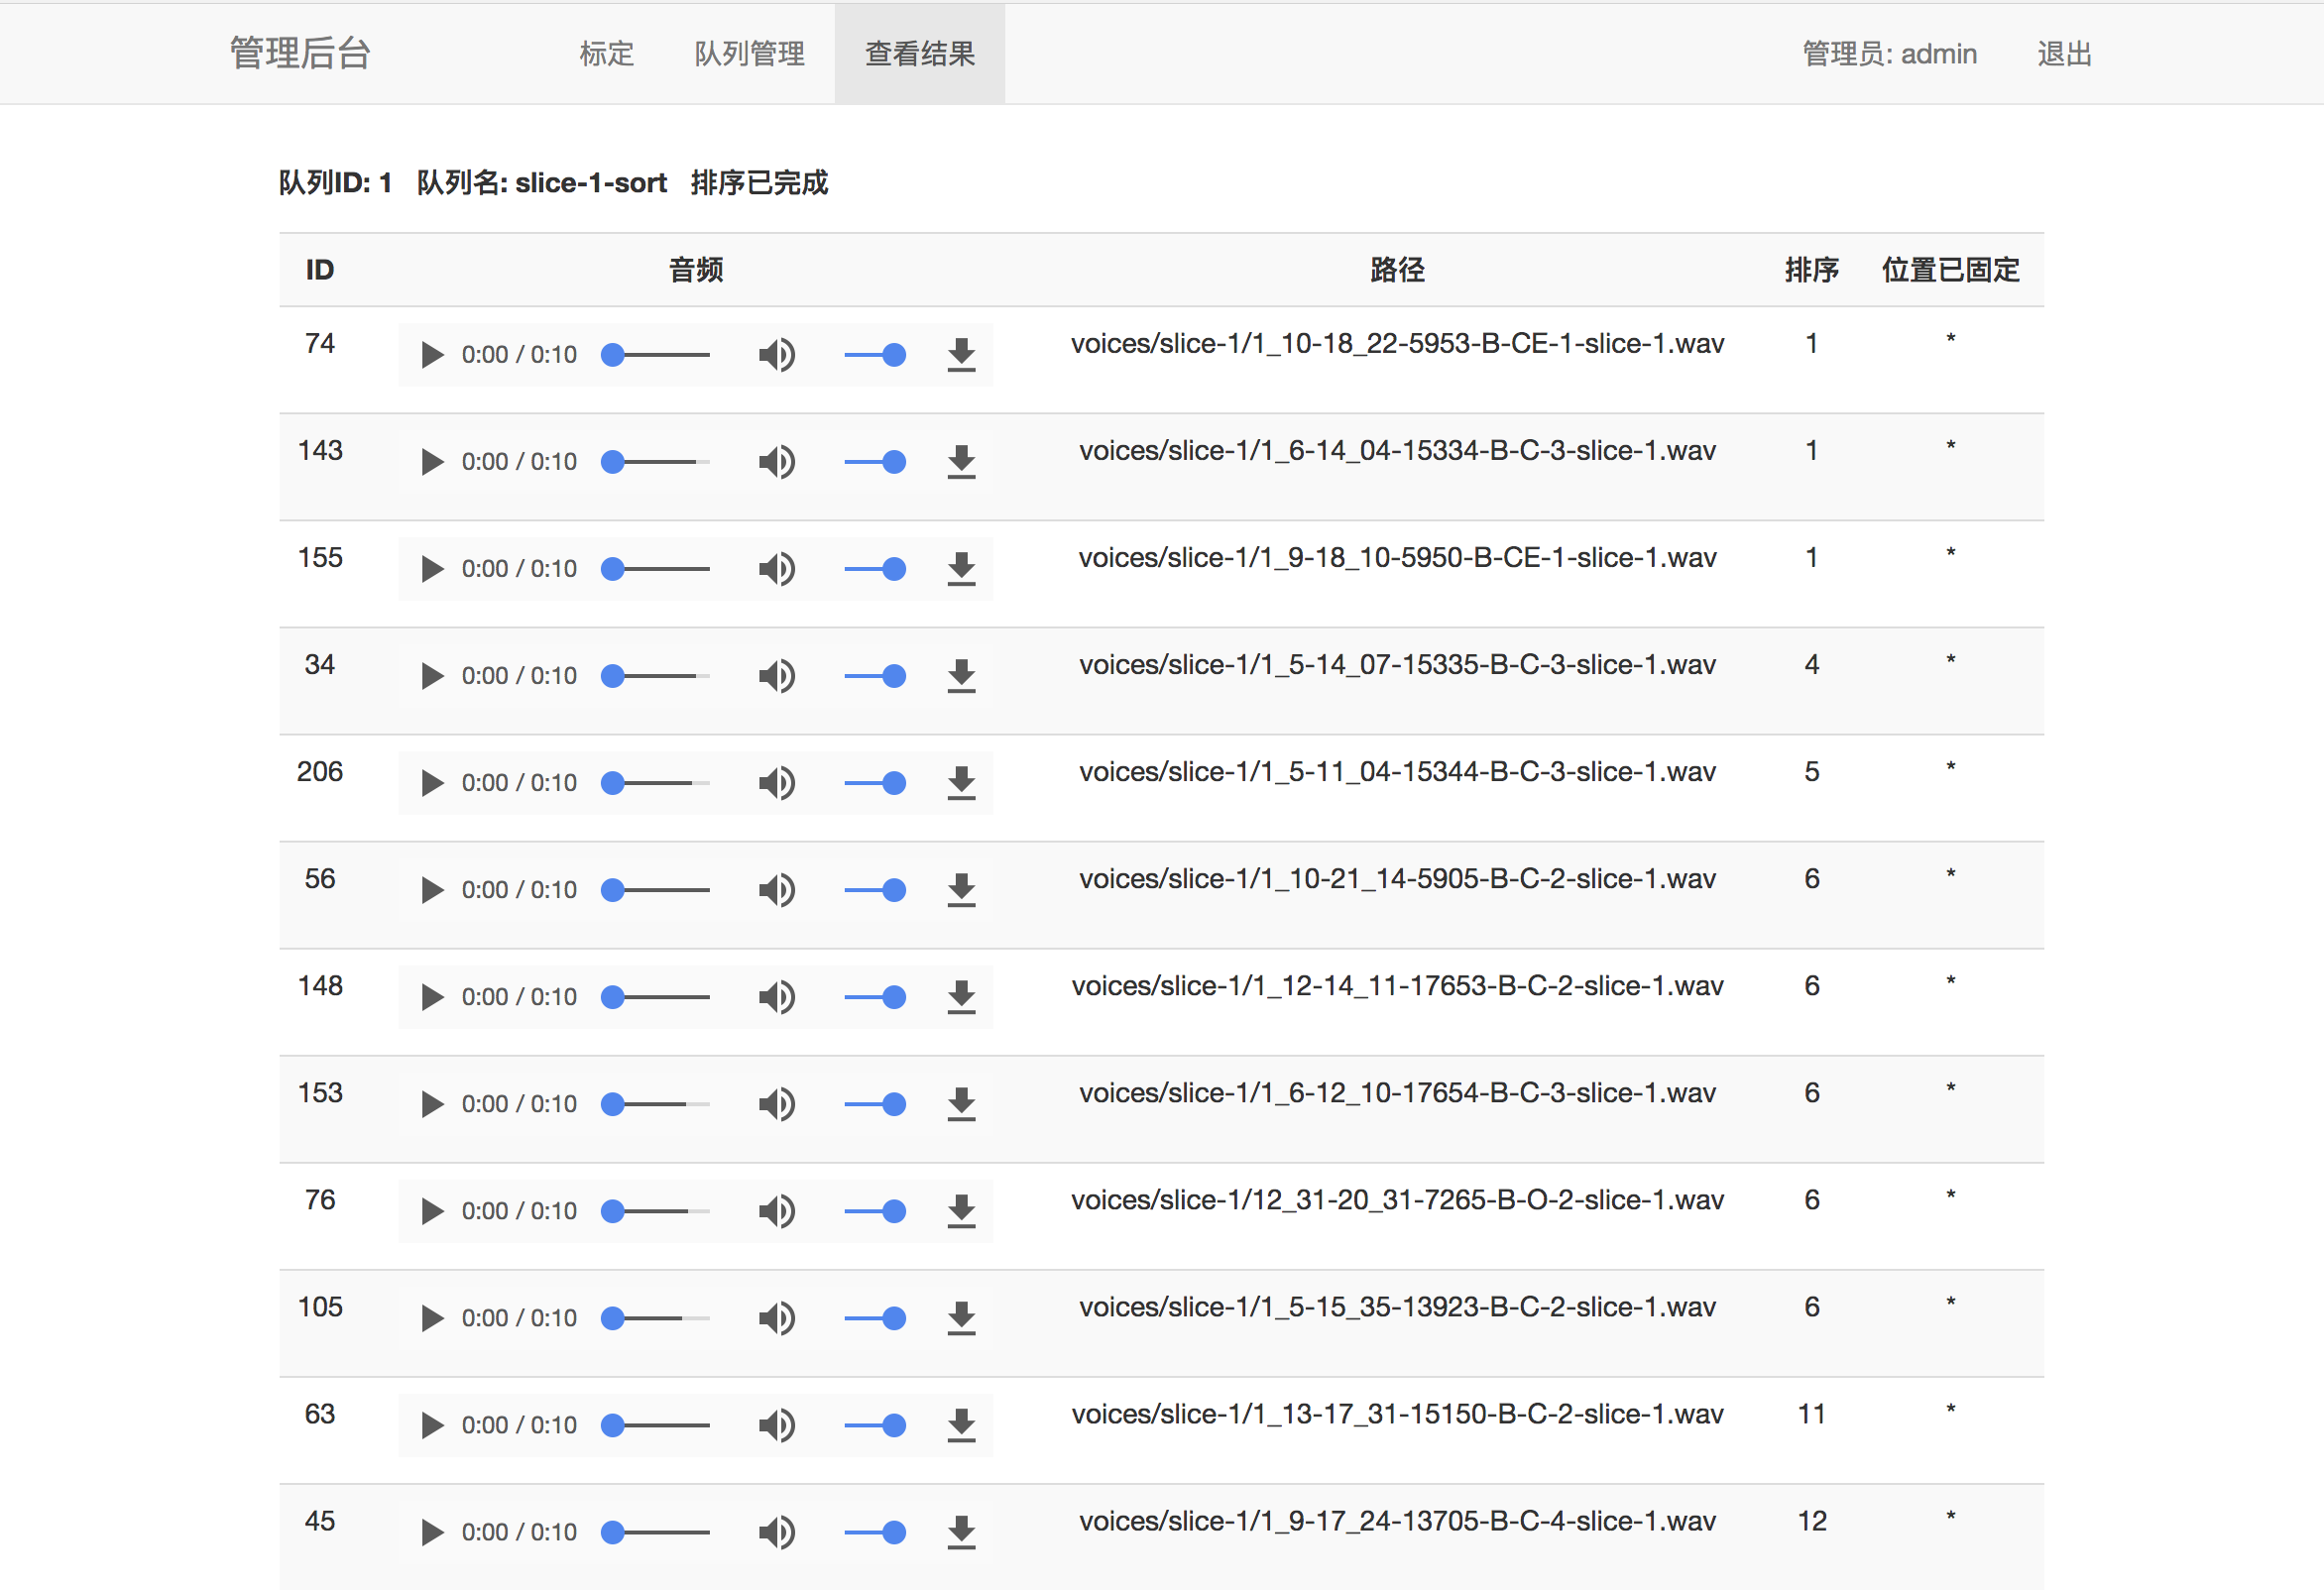
\includegraphics[width=0.8\textwidth]{web-sort}
}
\vspace{1.2ex}
\\
\subcaptionbox{MOS分结果\label{fig:web-mos}}{
    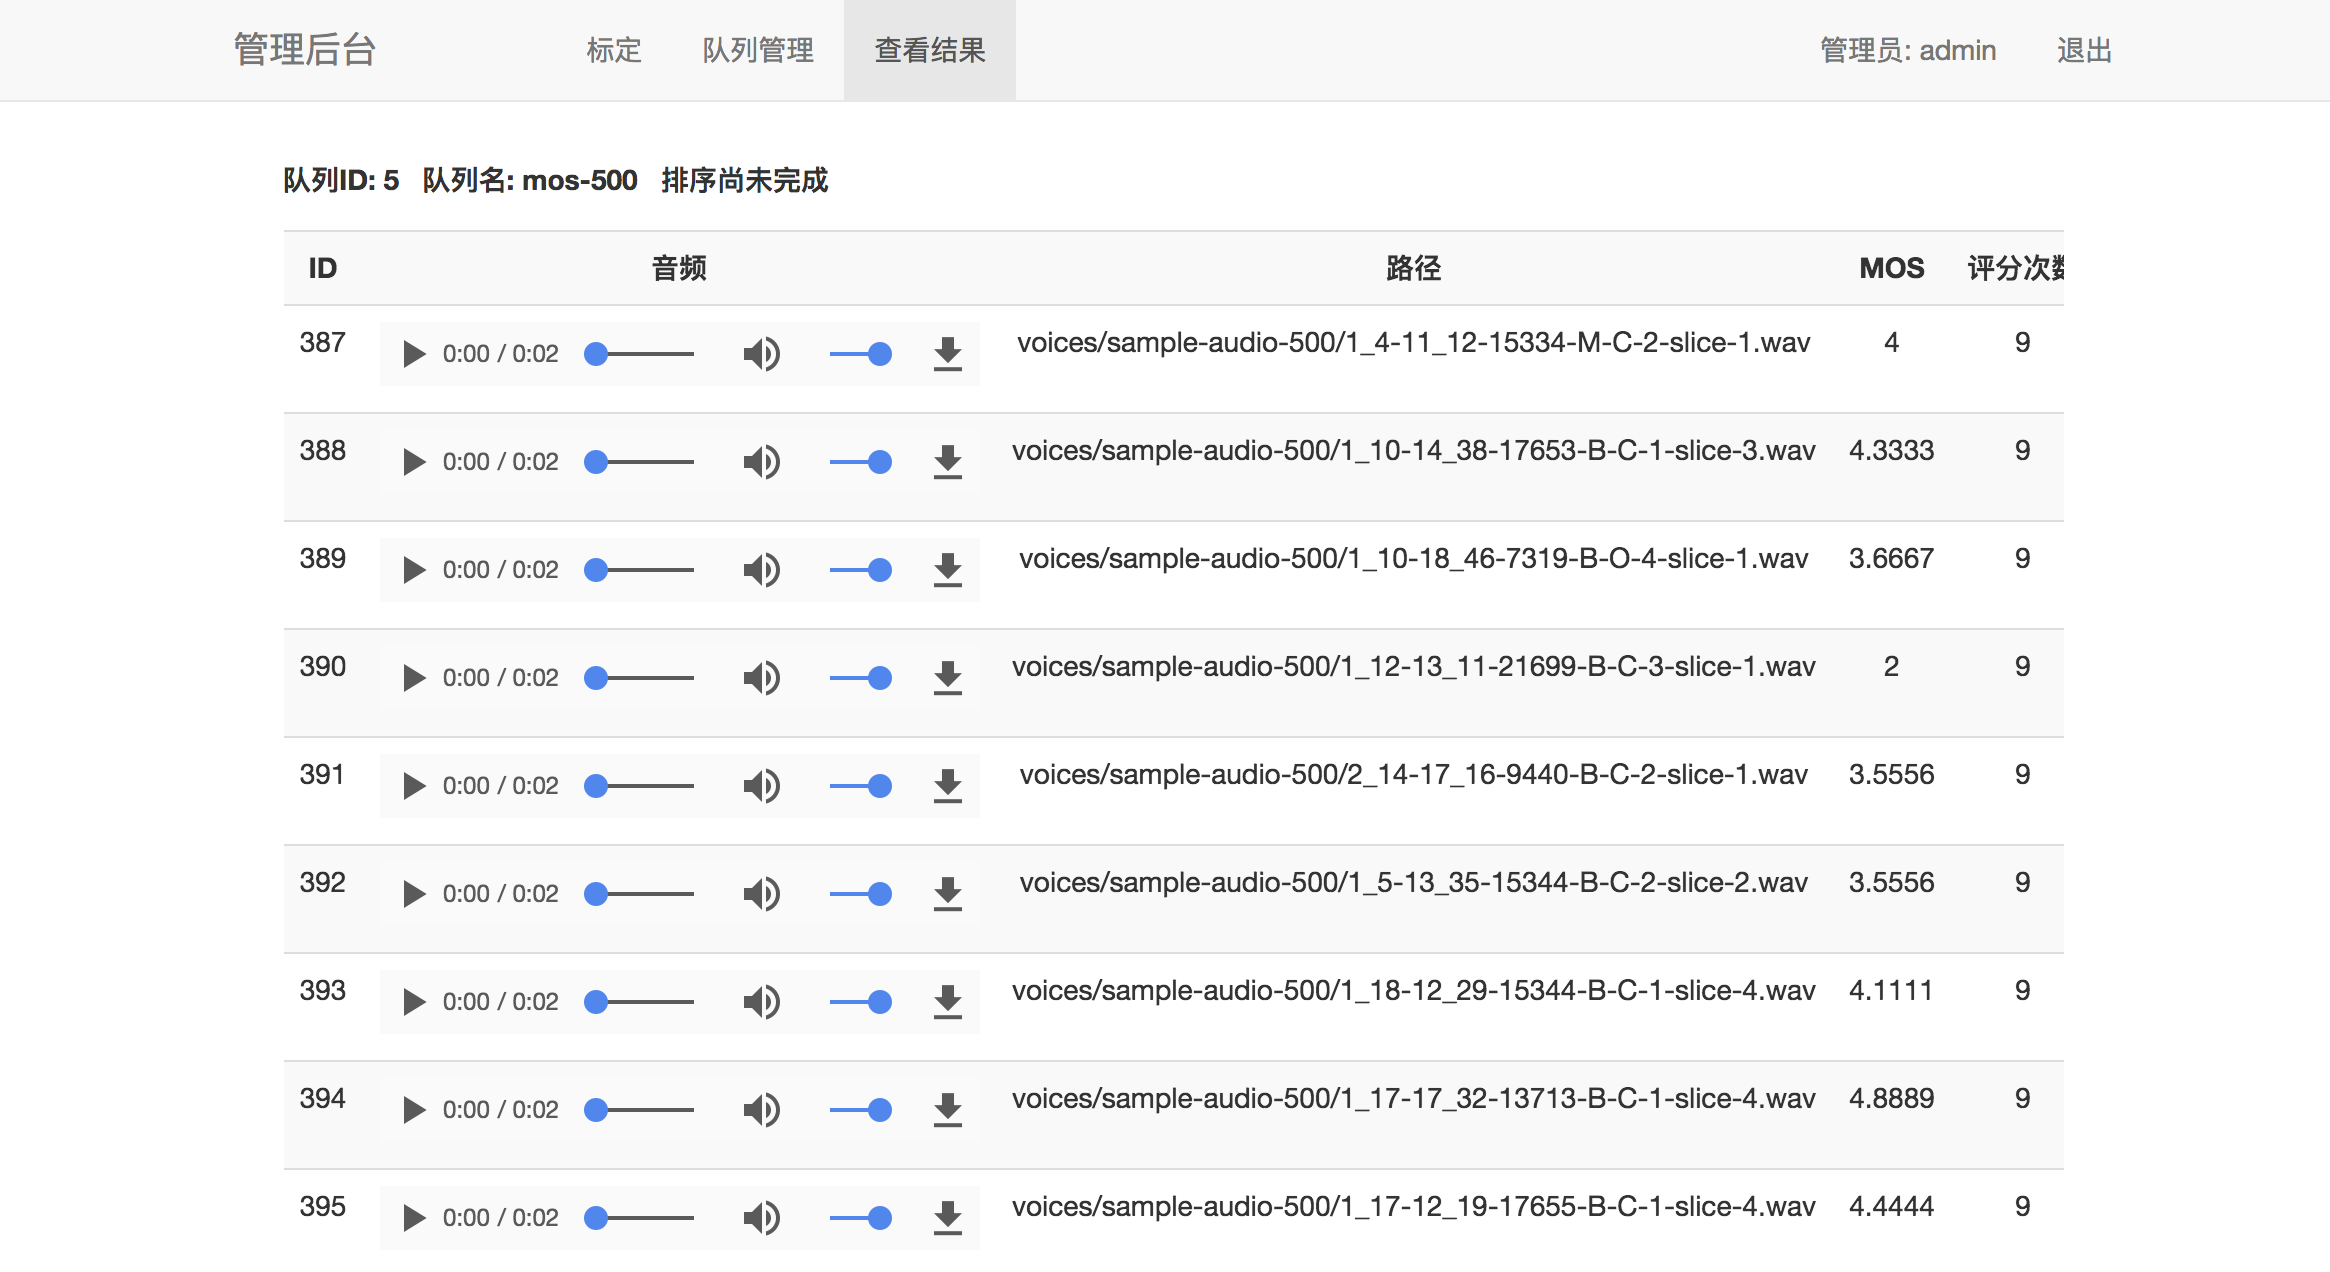
\includegraphics[width=0.8\textwidth]{web-mos}
}
\vspace{0.8ex}
\\
\caption{在线辅助系统的队列结果界面\label{fig:web-result}}
\end{figure}

\begin{figure}
\centering
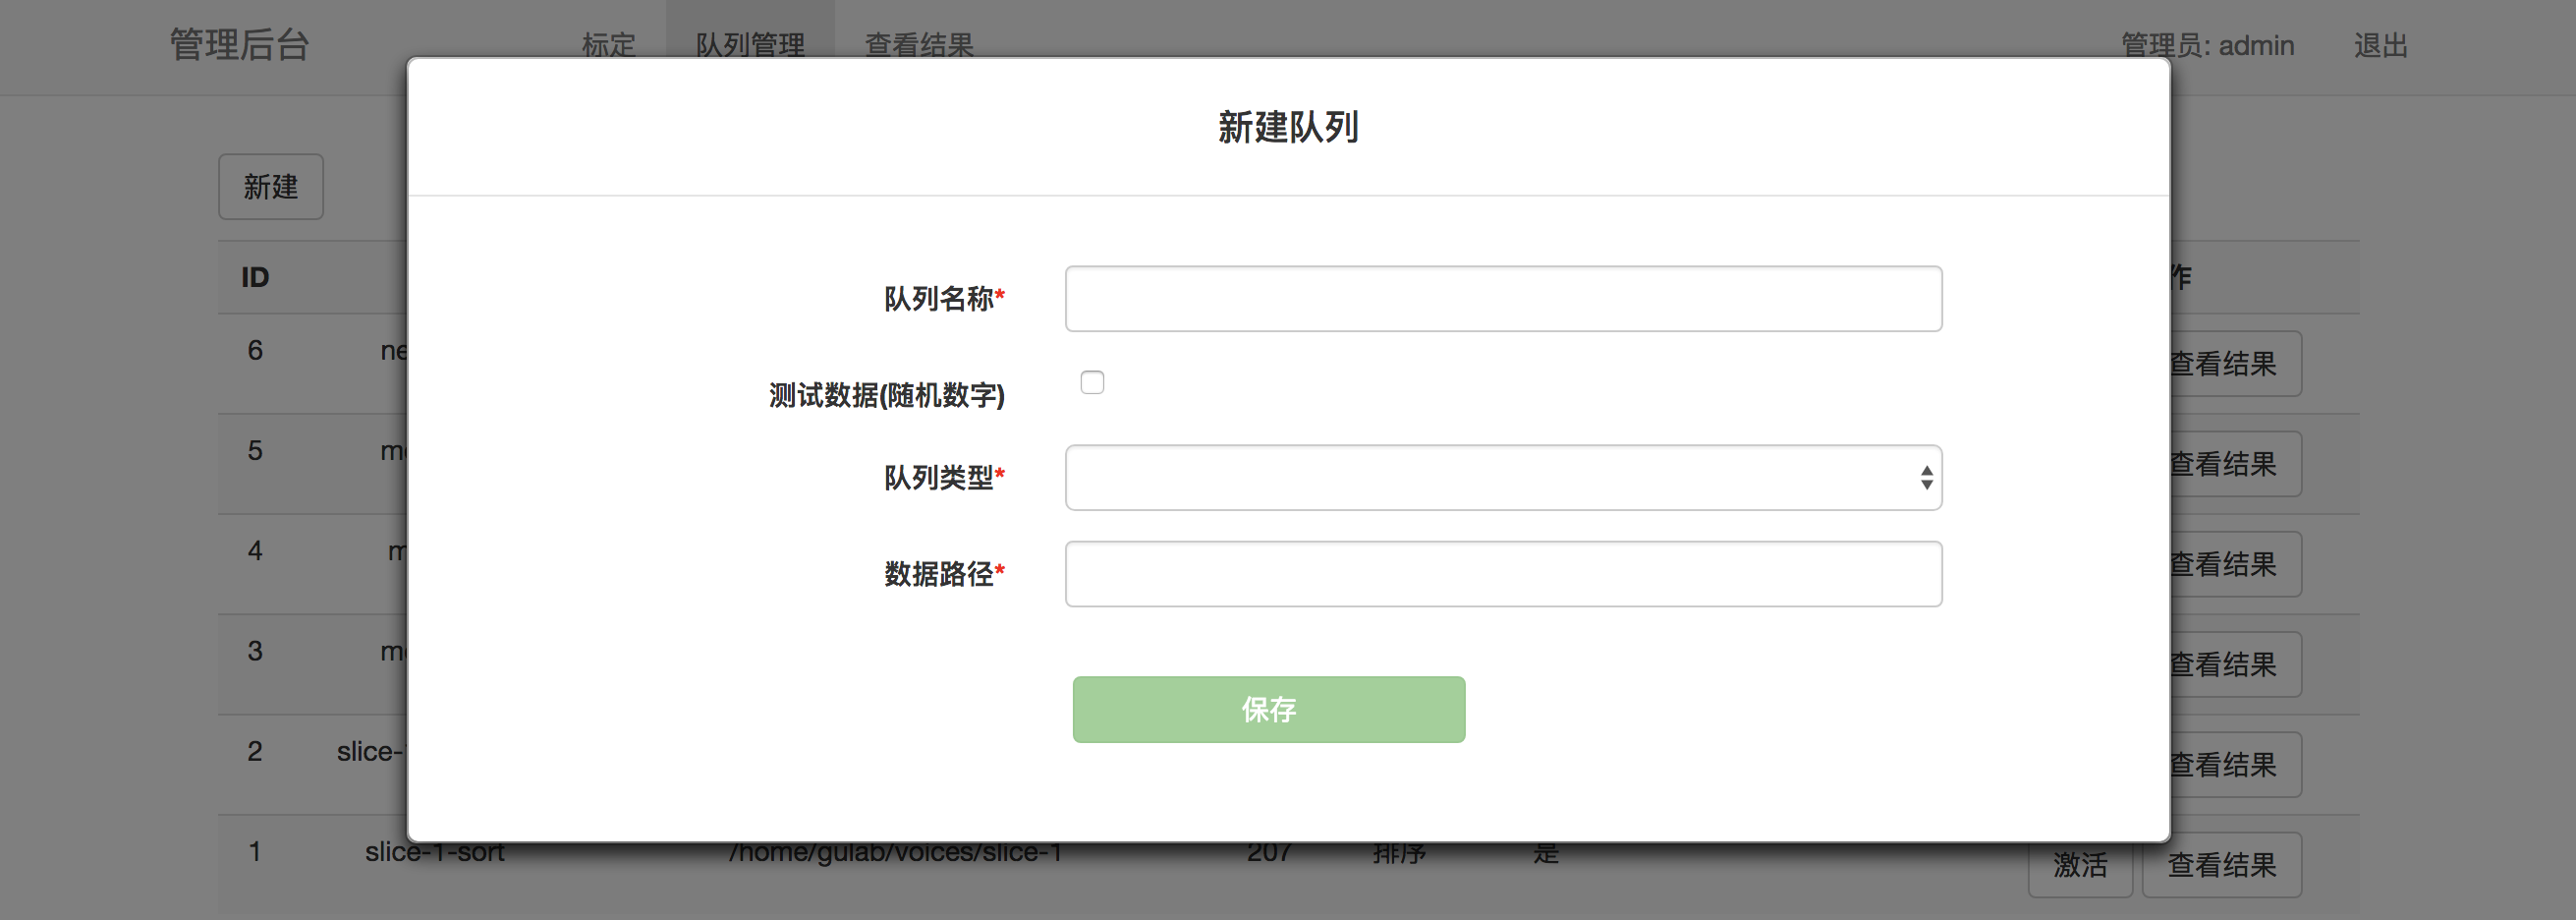
\includegraphics[width=0.8\textwidth]{web-new-queue}
\caption{在线辅助系统的新建队列界面\label{fig:web-new-queue}}
\end{figure}

管理端可以查看所有进行中和过往的主观评价实验,如图~\ref{fig:web-queues}所示,一次主观评价实验包含一系列短波语音,称为一个“语音队列”。队列类型有两种:“排序”、“MOS分”,分别对应于系统的两种功能。当前活跃的队列为正在进行的实验,志愿者看到的问题来自于该实验。可以点击“激活”来切换活跃的队列,点击“查看结果”来查看某一次实验的结果。点击“新建”按钮可以新建一个主观评价实验的语音队列。

图~\ref{fig:web-sort}为某一排序实验的结果,“排序”一列显示的是该语音在此队列中排序的位置,可以存在并列的情况。图~\ref{fig:web-mos}为某一MOS分实验结果,“MOS”一列表示当前计算的语音的MOS分,而“评分次数”表示当前完成对该语音的评分的志愿者数量。以上结果均可使用脚本进行导出,方便进一步基于主观评价结果的研究和实验。

图~\ref{fig:web-new-queue}为新建队列的界面,输入语音队列的名称,数据路径,选择实验类型,即可新建队列。系统后台会自动扫描数据路径下的语音数据,在系统中新建实验队列。

\begin{figure}
\centering
\subcaptionbox{排序任务\label{fig:web-user-sort}}{
    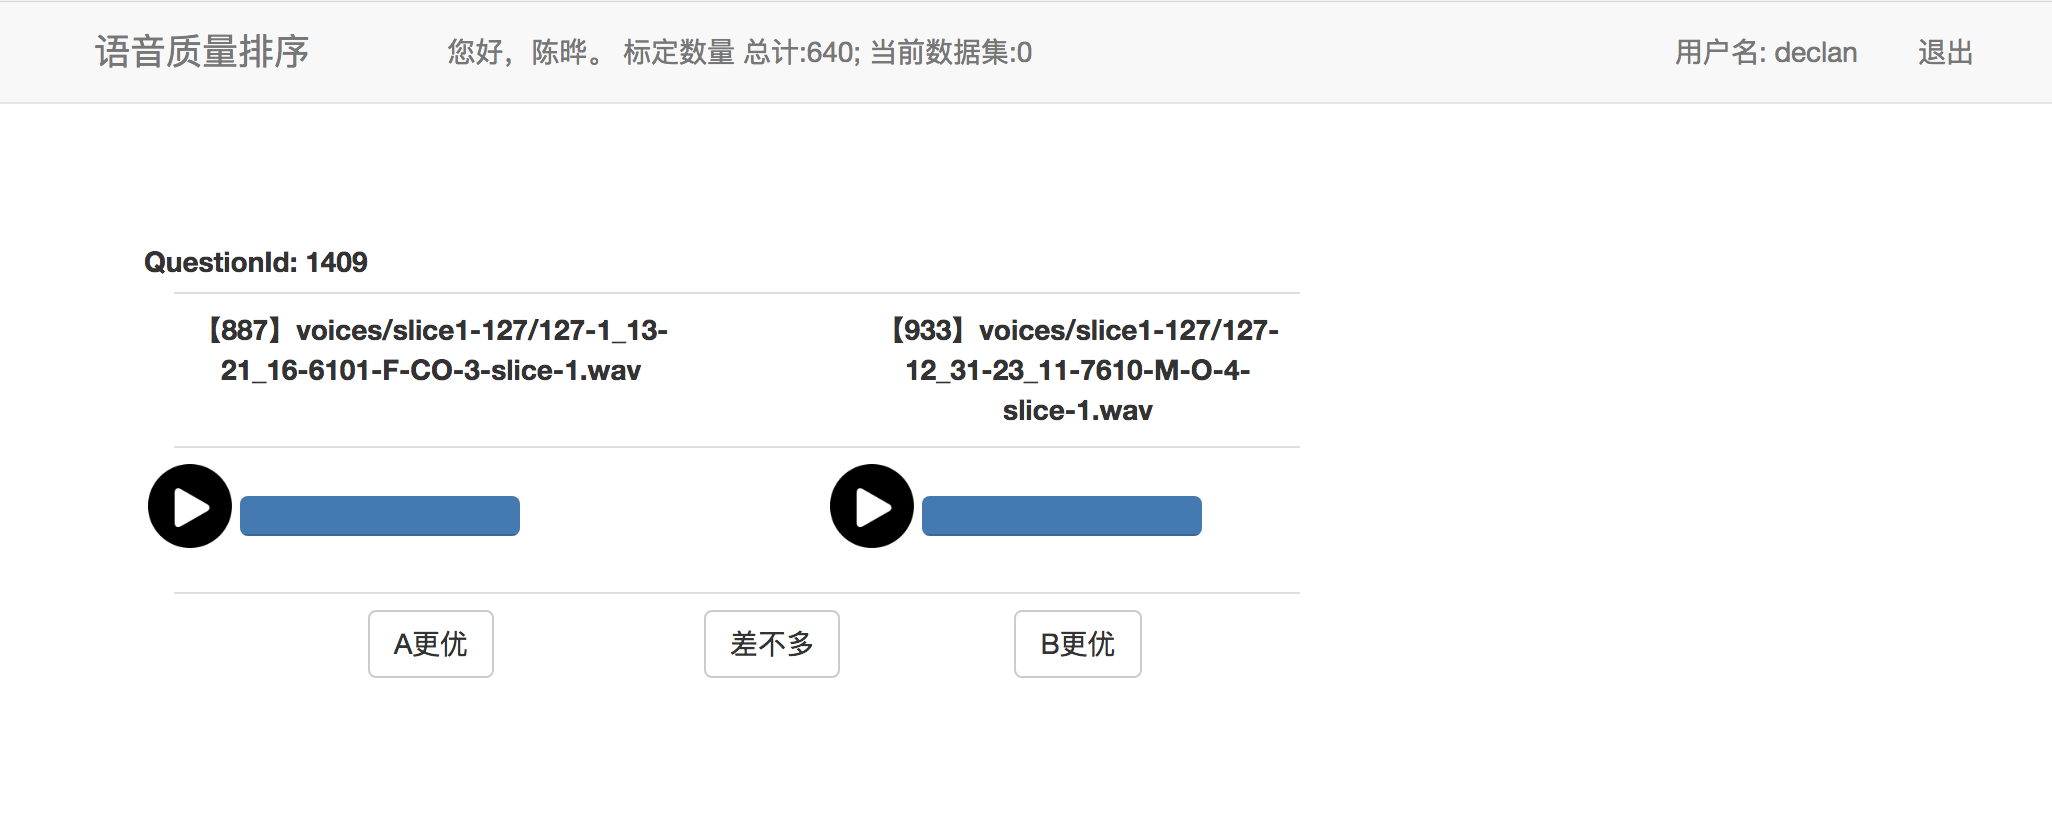
\includegraphics[width=0.8\textwidth]{web-user-sort}
}
\vspace{1.2ex}
\\
\subcaptionbox{MOS分任务\label{fig:web-user-mos}}{
    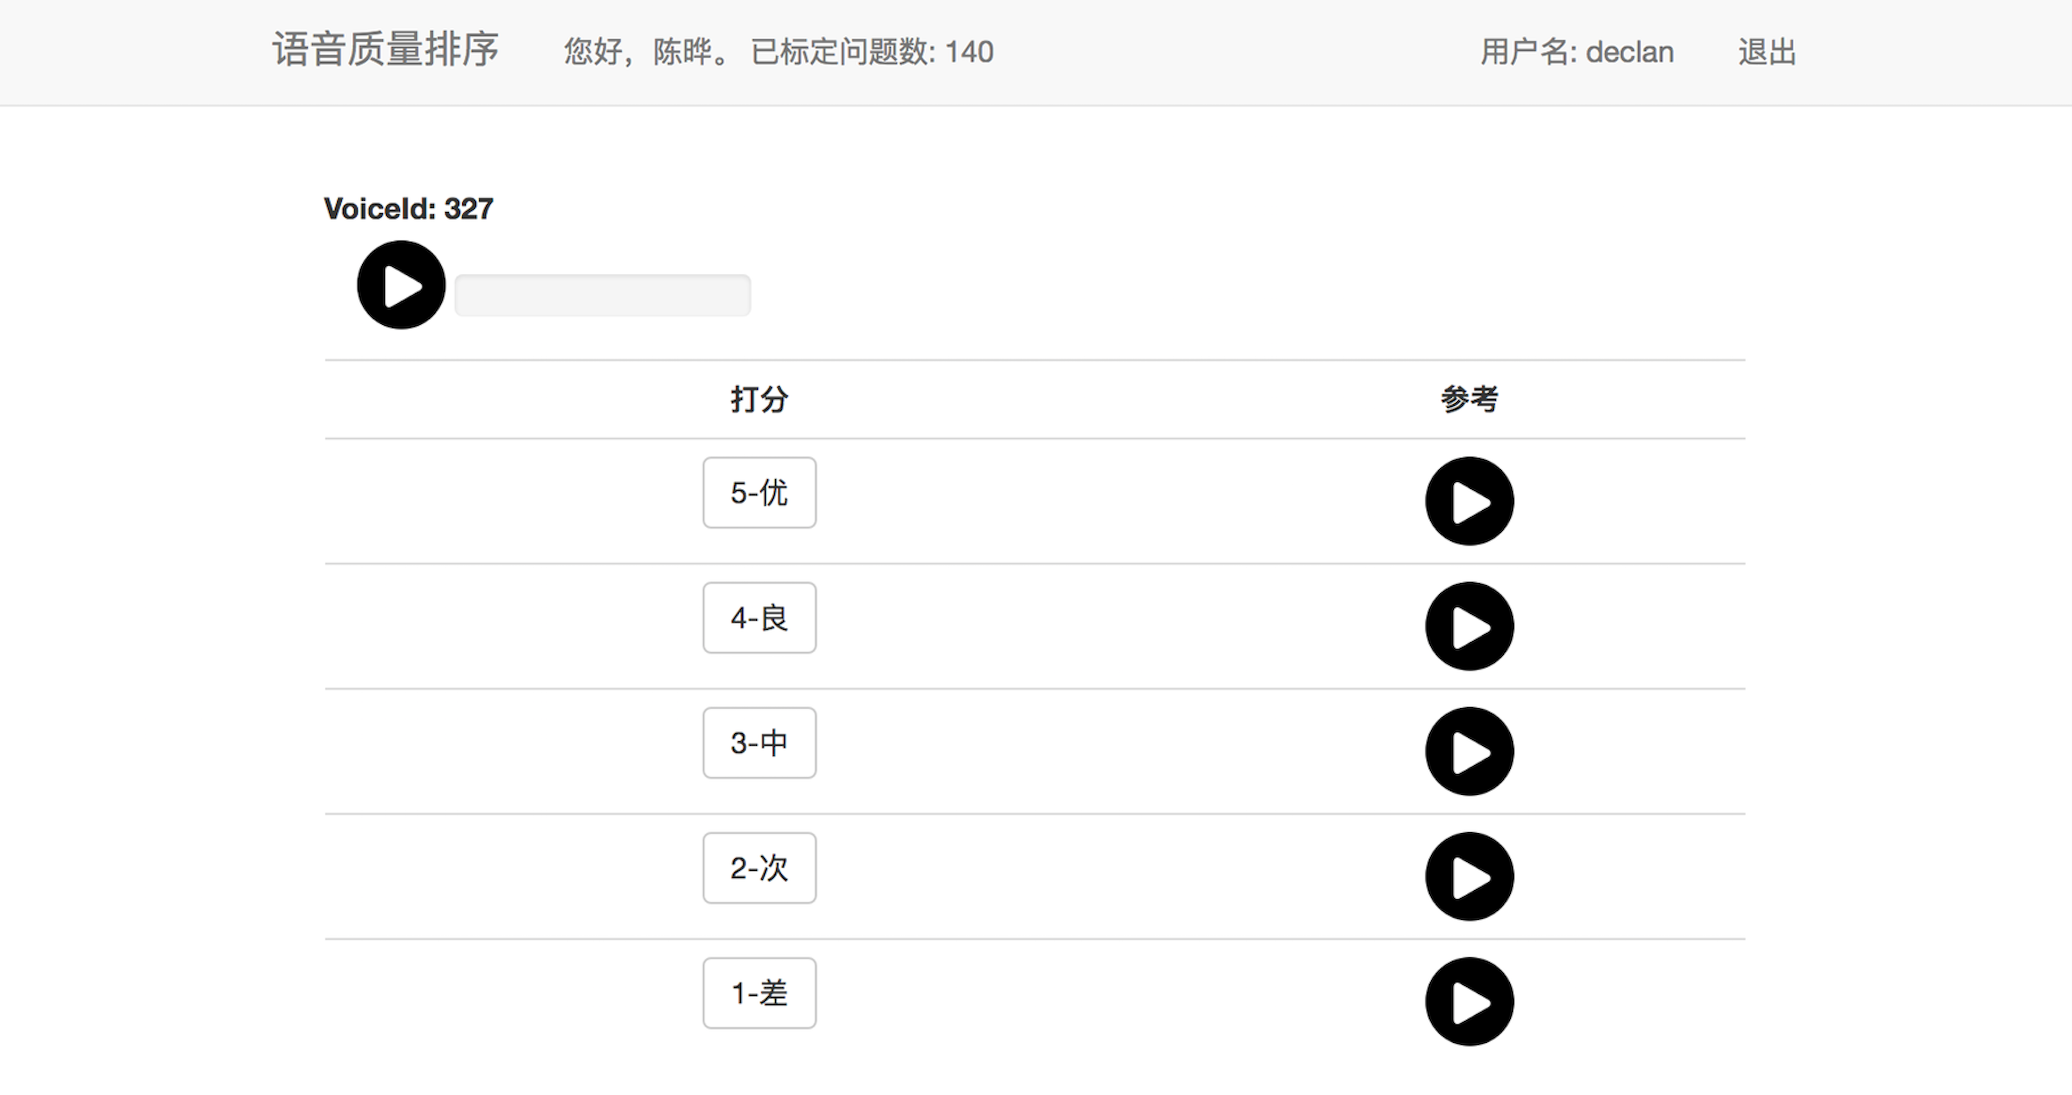
\includegraphics[width=0.8\textwidth]{web-user-mos}
}
\vspace{0.8ex}
\\
\caption{在线辅助系统的志愿者界面\label{fig:web-user}}
\end{figure}

志愿者端则是会显示当前需要完成的主观评分或者比较的问题,供志愿者回答,如图~\ref{fig:web-user}所示,志愿者界面上方显示了志愿者的姓名,已经标定的问题数量等信息。在排序任务中,志愿者的界面如图~\ref{fig:web-user-sort}所示,系统会让志愿者试听两个短波语音,让志愿者选择哪一个质量更优,或者选择两者质量差不多。而在MOS分任务中,志愿者的界面如图~\ref{fig:web-user-mos}所示,系统会给出一个待评分的语音,志愿者对其进行质量评分,选择1~5中的一个分数。每个分数右侧会有预先分组好的各等级语音的参考标准,供志愿者试听比较从而更好的进行评判。志愿者每回答完一个问题,会显示新的问题,直至当前实验中的任务均已完成为止。

\section{系统实现介绍}

短波语音主观评价在线辅助系统实现在Ubuntu 14.04操作系统上,基本环境要求如下:
\begin{itemize}
    \item 操作系统:Ubunutu 14.04
    \item Web服务器: Jetty9.2.24
    \item Java: JRE 7
    \item 数据库:MySQL 5.5
\end{itemize}

系统后端使用Java的Spring框架和Jersey框架实现符合Restful~\cite{fielding2000rest}设计理念的API接口,前端使用AngularJs实现单页web应用,符合MVC~\cite{leff2001web}设计模型,将系统的数据层、逻辑层和表示层完全剥离解耦~\cite{burbeck87}。数据库部分使用MySQL数据库存储,包括账户信息数据表、语音队列数据表、语音数据表、语音比较问题表、语音主观评分表,分别如表~\ref{tab:user}\~~\ref{tab:score}所示。

\begin{table}
\centering
\caption{账户信息数据表vs\_user}
\label{tab:user}
\begin{tabular}{ccc}
\toprule[1.5pt]
字段名 & 字段类型 & 备注 \\ \midrule[1pt]
u\_id & bigint(20) & Unsigned, Primary key, Auto Increment \\
u\_username & varchar(255) & 用户名 \\
u\_password & varchar(128) & 加密存储的密码 \\
u\_name & varchar(255) & 真实姓名 \\
u\_role & tinyint(3) & 0: 志愿者,1:管理员 \\
u\_answer\_cnt & int(10) & 回答问题数量 \\
u\_createtime & timestamp & 默认current\_timestamp \\ \bottomrule[1.5pt]
\end{tabular}
\end{table}

\begin{table}
\centering
\caption{语音队列数据表vs\_queue}
\label{tab:queue}
\begin{tabular}{ccc}
\toprule[1.5pt]
字段名 & 字段类型 & 备注 \\ \midrule[1pt]
q\_id & bigint(20) & Unsigned, Primary key, Auto Increment \\
q\_name & varchar(255) & 语音队列的名称 \\
q\_data\_path & varchar(255) & 语音文件的存储目录 \\
q\_length & int(10) & 队列长度(包含语音数量) \\
q\_type & tinyint(4) & 队列类型,0: 排序类型,1: MOS分类型 \\
q\_sorted & tinyint(1) & 排序是否已完成,仅对排序类型有效 \\
q\_active & tinyint(1) & 是否当前激活队列 \\
q\_createtime & timestamp & 默认current\_timestamp \\ \bottomrule[1.5pt]
\end{tabular}
\end{table}

\begin{table}
\centering
\caption{语音数据表vs\_voice}
\label{tab:voice}
\begin{tabular}{ccc}
\toprule[1.5pt]
字段名 & 字段类型 & 备注 \\ \midrule[1pt]
v\_id & bigint(20) & Unsigned, Primary key, Auto Increment \\
v\_queue\_id & bigint(20) & 所属队列的id,对应vs\_queue表中的q\_id字段 \\
v\_path & varchar(255) & 语音文件的存储路径 \\
v\_order & bigint(20) & 当前在队列中所处排序位置 \\
v\_fixed & tinyint(1) & 当前排序位置是否已固定 \\
\end{tabular}
\end{table}

\begin{table}
\centering
\caption{语音比较问题表vs\_compare}
\label{tab:compare}
\begin{tabular}{ccc}
\toprule[1.5pt]
字段名 & 字段类型 & 备注 \\ \midrule[1pt]
c\_id & bigint(20) & Unsigned, Primary key, Auto Increment \\
c\_queue\_id & bigint(20) & 所属队列的id,对应vs\_queue表中的q\_id字段 \\
c\_vid1 & bigint(20) & 待比较语音1的id,对应vs\_voice表中的v\_id字段 \\
c\_vid2 & bigint(20) & 待比较语音2的id,对应vs\_voice表中的v\_id字段 \\
c\_result & tinyint(4) & 比较结果,0:差不多,1:语音1质量更好,2:语音2质量更好 \\
c\_answer\_uid & bigint(20) & 回答者的id,对应vs\_user表中的u\_id字段 \\
c\_post\_time & timestamp & 该问题最近一次被志愿者获取的时间 \\ \bottomrule[1.5pt]
\end{tabular}
\end{table}

\begin{table}
\centering
\caption{语音主观评分表vs\_score}
\label{tab:score}
\begin{tabular}{ccc}
\toprule[1.5pt]
字段名 & 字段类型 & 备注 \\ \midrule[1pt]
s\_id & bigint(20) & Unsigned, Primary key, Auto Increment \\
s\_userid & bigint(20) & 评分志愿者的id,对应vs\_user表中的u\_id字段 \\
s\_queueid & bigint(20) & 所属队列的id,对应vs\_queue表中的q\_id字段 \\
s\_voiceid & bigint(20) & 评分语音的id,对应vs\_voice表中的v\_id字段 \\
s\_score & int(11) & 评分结果 \\
s\_post\_time & timestamp & 评分时间 \\ \bottomrule[1.5pt]
\end{tabular}
\end{table}

\subsection{语音质量排序的实现}

为了实现对短波语音按照主观感受质量进行排序,我们首先基于快速排序算法~\cite{hoare1962quicksort}的思想设计了模糊版本快速排序算法,然后利用数据库和网站技术交互式地实现了该算法,使算法中的原子比较步骤由志愿者在网页进行,而排序算法由后端程序基于数据库记录的数据进行。

首先简单介绍一下快速排序算法的思想,快速排序是采用分治思想的一种排序算法,时间复杂度为$O(NlogN)$。该算法首先选取待排序元素的第一个或随机的一个作为基准元素,然后通过一次$O(N)$时间复杂度的扫描操作,可以确定该元素按照顺序在队列中的位置,同时保证此时在该元素前的元素均比其小,而在该元素之后的元素均比其大,该元素位置固定不动,将队列分成了前后两半,只有递归地对前后两半分别进行此扫描操作,直至所有元素均确定了位置,则排序完成。

\begin{algorithm}
    \caption{模糊快排中的扫描算法}
    \label{alg:fuzzy-sort}
\begin{algorithmic}[1]
\INPUT
    \Statex 待排序队列x[];
    \Statex 待排序区间$[l, r]$;
\OUTPUT
    \Statex 将x[]在$[l, r]$区间内分成$[l, i], [i+1,  j-1], [j, r]$三个区间
    \Statex $[i+1,  j-1]$中的元素均模糊相等
    \Statex $[l, i]$中的元素比上述元素小,$[l, i]$中的元素比上述元素大
\State 基准元素$y = x[l]$
\State $i=l-1, j=r+1, k=l$
\While { $k<j$ 且 $k\leq r$}
    \If { $x[k]<y$; }
        \State 交换$x[i+1], x[k]$的值
        \State $i = i + 1, k = k + 1$
    \ElsIf { $x[k] > y$; }
        \State 交换$x[j-1], x[k]$的值
        \State $j=j-1$
    \Else
        \State (x[k]和y模糊相等) $k=k+1$ 
    \EndIf
\EndWhile
\end{algorithmic}
\end{algorithm}

在语音的主观质量排序中,经常会出现两个语音质量近似相等,难以区分哪一个更优的情况,本文针对此优化设计了模糊版本的快速排序算法,此算法与快速排序算法的很接近,唯一的修改是在每次扫描时,将待排序的区间$[l, r]$划分成$[l, i], [i+1,  j-1], [j, r]$三个区间,其中$[l, r]$中的元素均是比基准元素小的,$[j, r]$中的均是比基准元素大的,而$[i+1,  j-1]$中是与基准元素模糊相等的。之后递归的对左区间和右区间进行扫描即可完成排序。改进的扫描算法的具体实现如算法~\ref{alg:fuzzy-sort}所示。

\begin{figure}
\centering
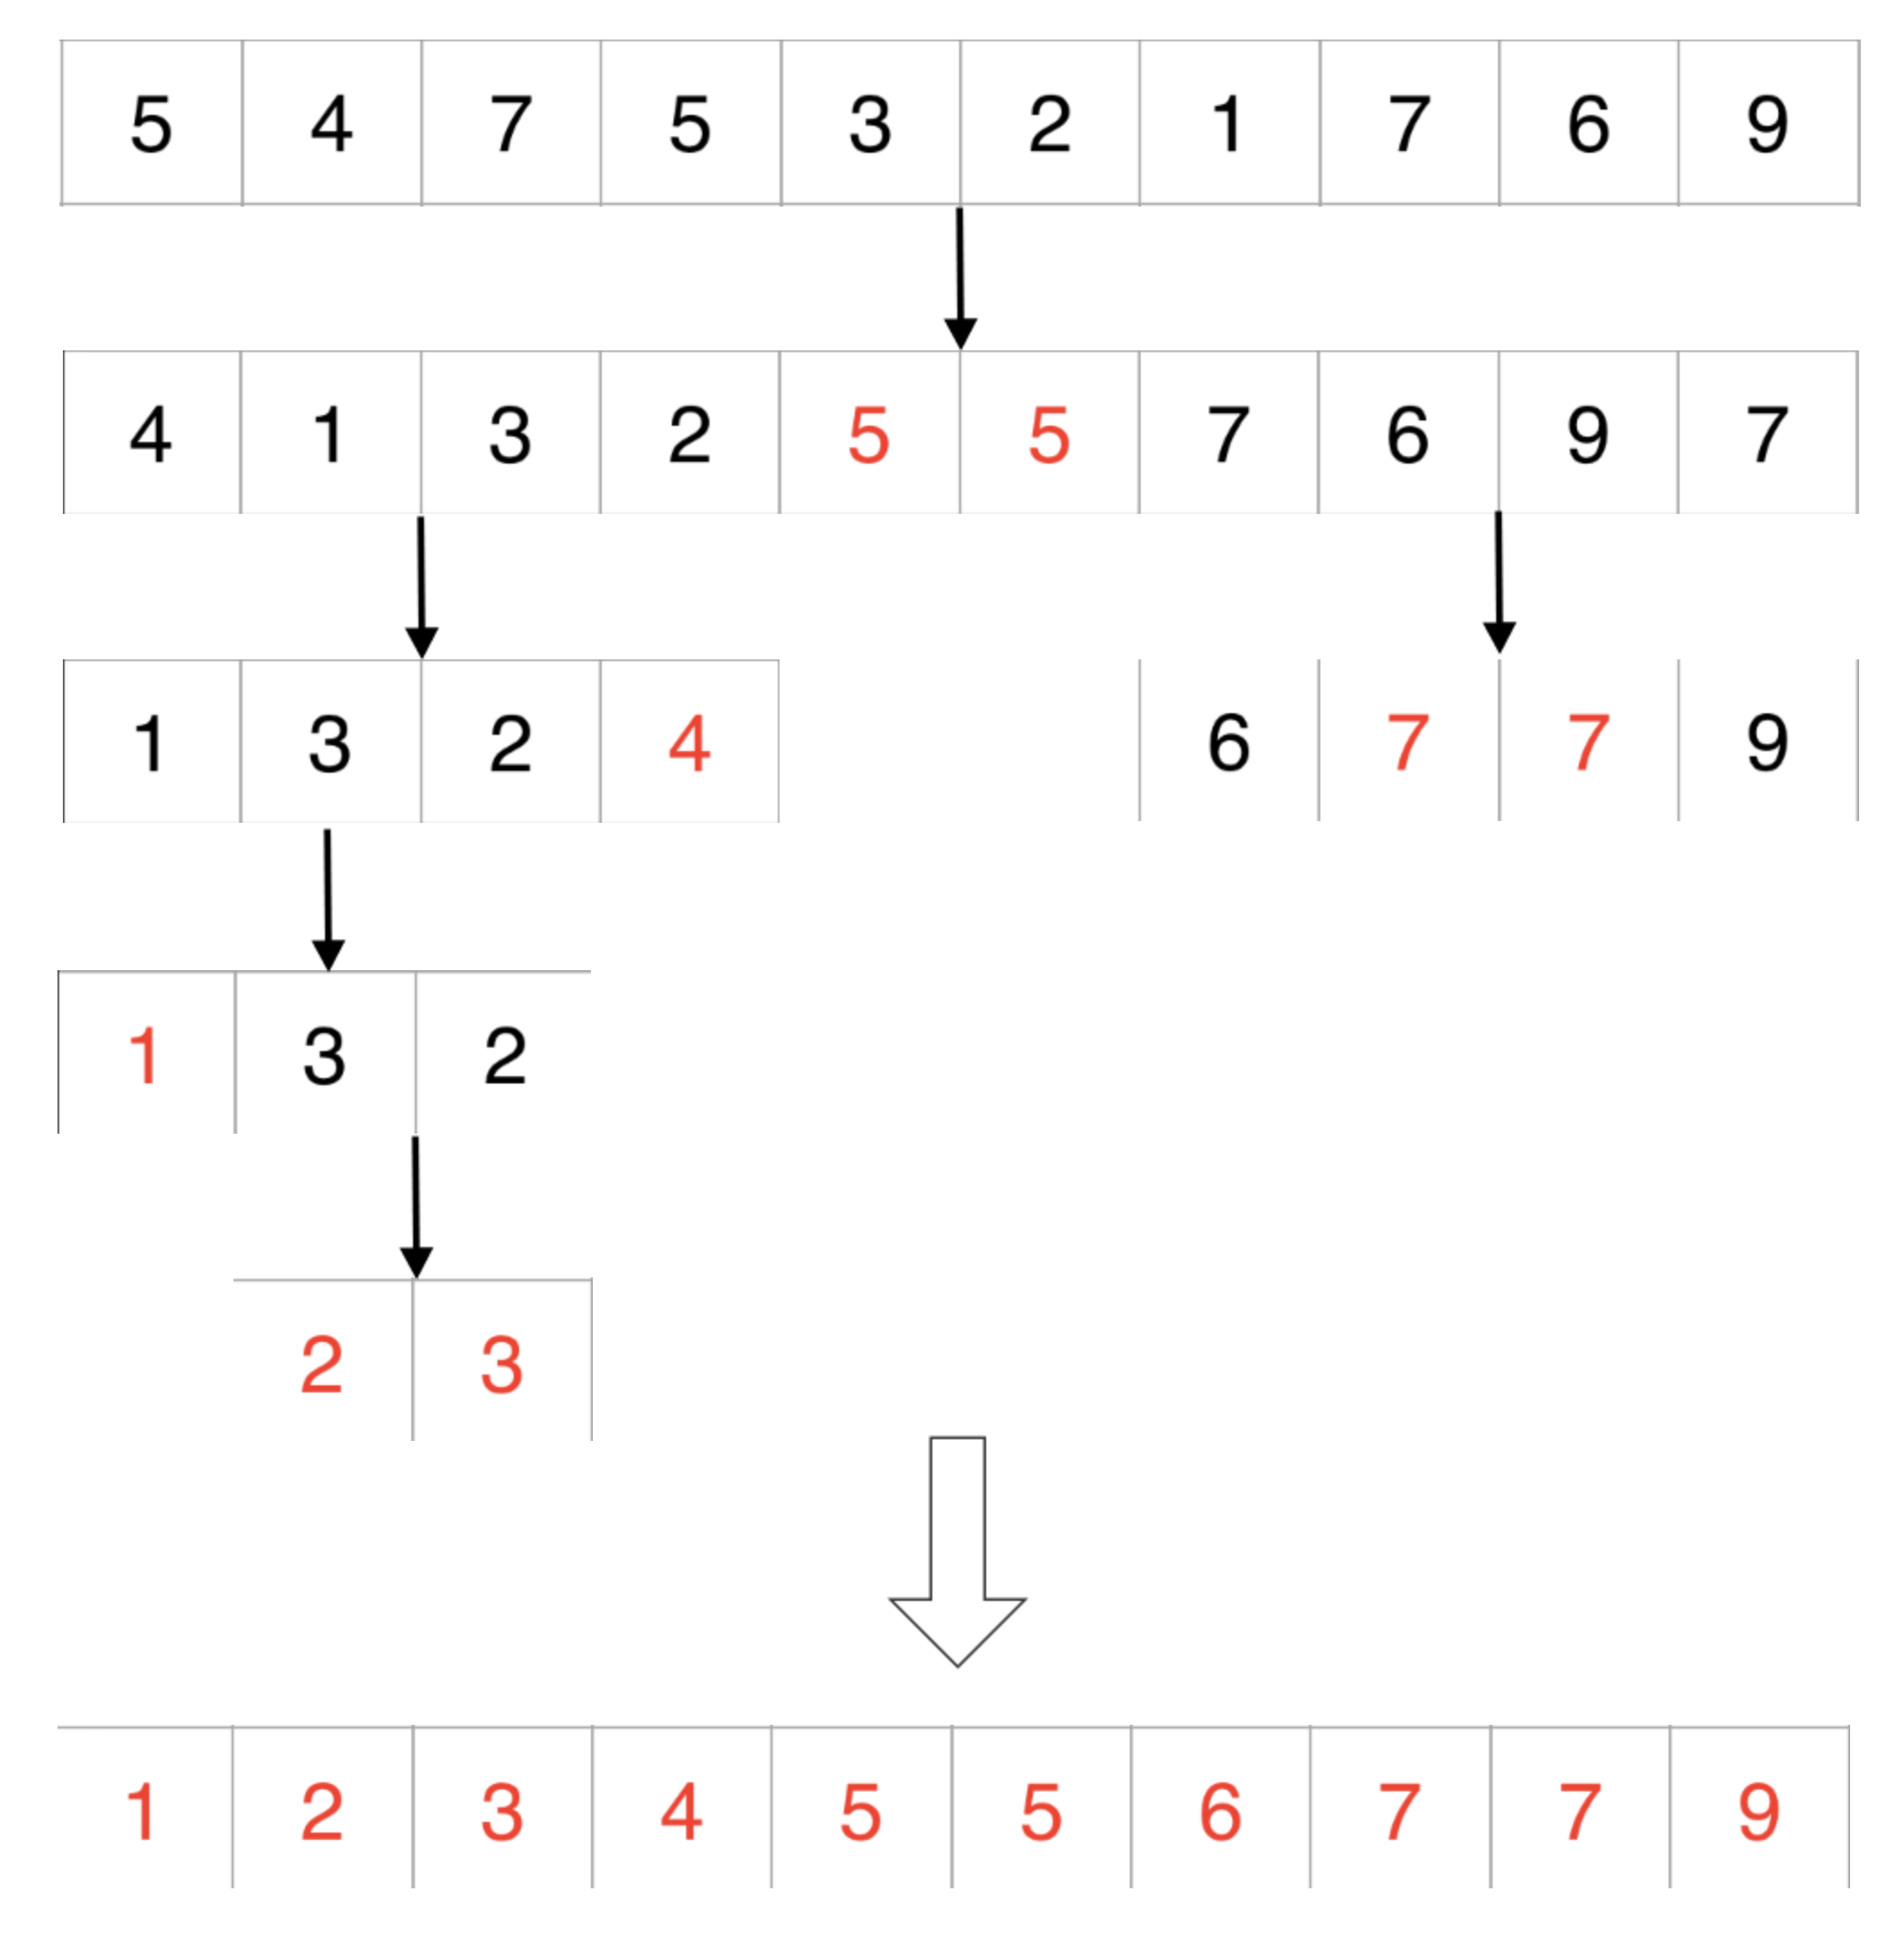
\includegraphics[width=0.6\textwidth]{sort-alg}
\caption{模糊快排算法执行示例\label{fig:fuzzy-sort}}
\end{figure}

图~\ref{fig:fuzzy-sort}演示了模糊快排算法对一列整数进行排序的过程,红色数字表示位置已经确定的数字。由于算法是递归执行,所以执行过程行成了一个树状结构。

\begin{algorithm}
    \caption{交互式模糊快排算法}
    \label{alg:interactive-sort}
\begin{algorithmic}[1]
\INPUT
    \Statex 待排序语音v[],总个数L
\OUTPUT
    \Statex 排序结果order[],对应每个语音的排序位置
\State 初始化order[]为1至L
\State fixed[]数组表示每个语音位置是否已固定,全部初始化为false
\While { $ \exists i, s.t. fixed[i] = false $; }
    \State 将order[]和fixed[]信息存储进vs\_voice表
    \State 根据当前排序状态,参考算法~\ref{alg:fuzzy-sort}生成所有需要比较的语音对,插入vs\_compare表
    \State 等待志愿者回答所有的语音质量比较问题
    \State 根据志愿者的回答,参考算法~\ref{alg:fuzzy-sort}更新所有待定区间的排序状态,更新order[]和fixed[]
\EndWhile
\end{algorithmic}
\end{algorithm}

将该算法应用到短波语音的主观质量排序中时,两个语音的质量比较过程需要由志愿者而非程序完成。所以我们设计了一个基于数据库存储和网站技术的交互式模糊快排算法。主要思想是将排序的递归树按层分,每一层的排序状态可以保存在数据库中。基于排序状态生成当前所有需要进行比较的语音对,将这些比较分发给志愿者回答。当所有问题均已被回答,程序从数据库中读取当前排序状态,根据回答的问题可以排序队列进入到下一层状态中。如此循环往复直至所有语音均排序完毕。具体的存储情况如下:vs\_voice表(参见表~\ref{tab:voice})中存储了每个语音在排序中的位置(v\_order字段),以及位置是否已经固定(v\_fixed字段),这两个信息即可保存队列排序的状态信息;而需要比较的语音对存储在vs\_compare表(参见表~\ref{tab:compare})中,志愿者回答的信息也会保存到该表中。具体算法流程如算法~\ref{alg:interactive-sort}所示。

上述算法中生成的语音比较问题会插入vs\_compare表,下面说明前端获取比较问题给志愿者回答的策略。我们希望尽量减少志愿者重复回答同一问题,所以首先获取没有被其他志愿者获取过的问题。而当目前所有问题均已被获取过,则获取最早分发给志愿者而依然没有被回答的问题。具体实现上在vs\_compare表中有c\_post\_time标记了该比较问题上一次被获取的时间,若还未被获取则为空(null),而c\_answer\_uid记录了回答该问题的志愿者id,如果还未被回答则为空(null)。我们根据这两个字段来获取当前该分发给志愿者的问题。

\subsection{语音MOS分评价的实现}

统计语音的平均主观意见分(MOS)的功能要相对简单一些,建立语音队列时,扫描目录下的语音文件,在vs\_voice中插入所有语音的数据记录。然后每个志愿者可以获取他还没有进行主观评分的语音,在前端展示试听,志愿者根据主观感受进行评分,分值从1-5不等。志愿者主观评分的记录被保存在vs\_score表中,通过统计该表信息,可以得到每条语音数据被几位志愿者评分,以及其平均主观意见分的分值。

\section{小结}

本章介绍了短波语音主观评价在线辅助系统。该系统用于辅助进行短波语音的主观评价工作,包含两种功能:一是通过主观比较对一组短波语音进行质量排序;二是通过记录统计主观评分计算各个短波语音的平均主观意见分。我们首先介绍了系统的功能和使用,然后介绍了系统的实现。
\chapter{实验和结果}\label{chapter:experiments}

为验证本文技术的效果,本文设计了两个实验,实验A用于验证客观评价算法的效果,实验B用于验证短波信道语音自动选路的最终效果。

实验A使用采集到的500个短波语音,分别使用客观评价算法、主观评价平台进行客观评分和主观评分。我们绘制主观评分结果和客观评分结果的线性回归图,分析客观评分和主观评分的相关关系,从而分析主观评价结果的好坏。此外我们将本文所提算法和两种标准客观评分算法的结果进行了比较。

实验B同时在多地采集同一短波信号,再使用本文的自动选路系统进行选路输出,对比最终结果语音和各路原始语音的质量,从而分析自动选路技术的效果优劣。

\section{实验数据采集}

由于没有现成的公开短波语音数据集,本文自建了一组短波语音的数据集并进行主观质量评分。

本文实验数据的采集,是使用短波收音机对各短波电台广播进行录音来获取的。在录音时使用音频线直接将短波收音机和录音笔连接起来,使用录音笔录音,从而避免引入附加的环境噪音。

对于实验A,我们在每天不同时段,对多个短波电台进行录音。然后对采集到的音频数据进行降采样,统一采样率为8kHz,再分割成每段2s的短语音,保存成“wav”格式。最终生成500个时长2s的短波语音片段。

对于实验B,由多人在2-3个城市,5-6个地点同时对同一频率的短波广播进行录音,各录音地点之间距离相隔不少于500m。对采集到的音频数据进行降采样,统一采样率为8kHz,分割成每段60s左右的语音,并保存为“wav”格式,命名形式为[时间]-[地点]-[频率]。

\section{实验A结果}

在实验A中,我们分别使用本文所提的两种客观评价算法对采集到的500个短波语音片段进行了客观质量评分。同时我们召集了16位志愿者,利用第~\ref{chapter:web}章介绍的在线辅助系统,对500个短波语音片段进行了平均主观意见分的评分。我们分别对两种算法的客观评分和主观评分进行了线性回归,结果如图~\ref{fig:regress}所示,其中每个蓝色散点代表一个语音片段,横坐标为算法客观评分结果,纵坐标为平均主观意见分,图中的红色直线为线性回归的结果。图~\ref{fig:regress1}为基于语谱图噪音模型的算法结果,图~\ref{fig:regress2}为基于自编码器的算法结果。从图中可以看出本文所提算法给出的语音质量客观评分能够反映出其主观感受质量的好坏。

\begin{figure}
\centering
\subcaptionbox{基于语谱图噪音模型的算法\label{fig:regress1}}{
    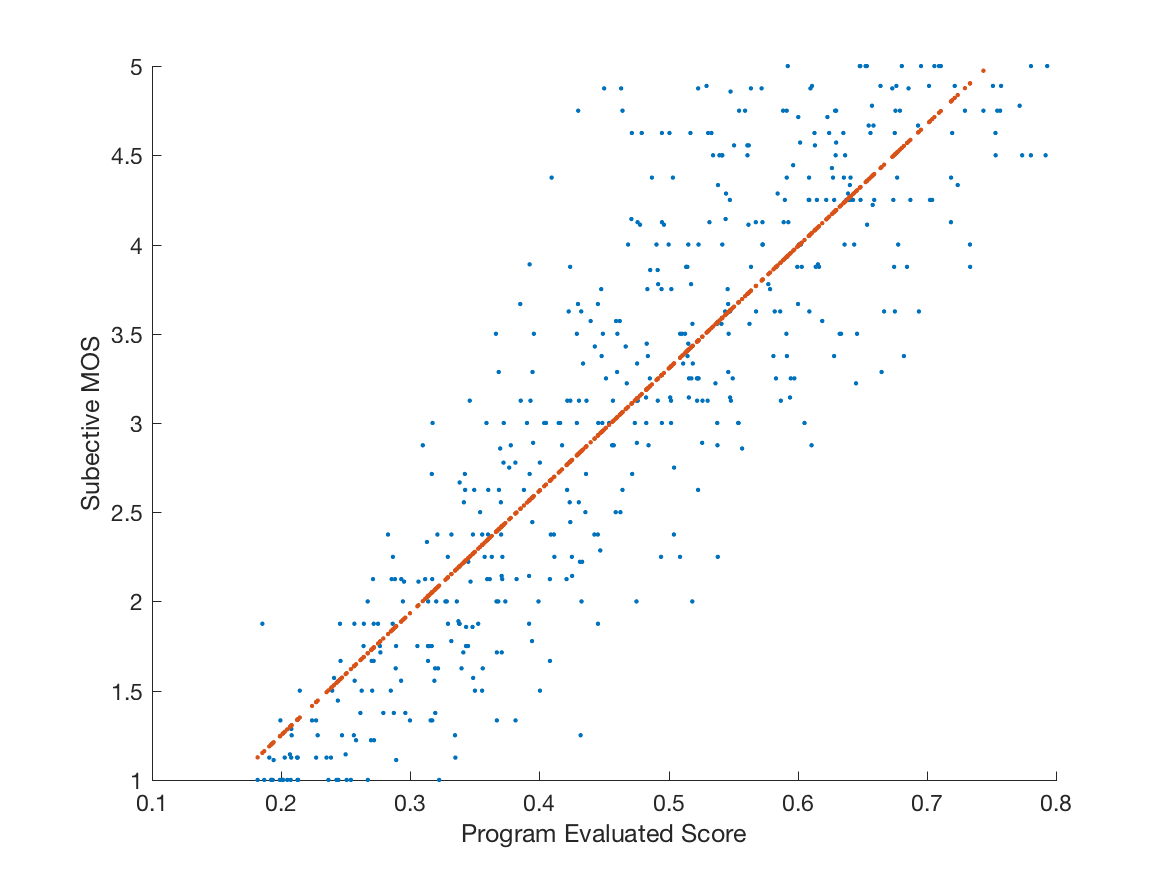
\includegraphics[width=0.8\textwidth]{regress}
}
\vspace{0.6ex}
\\
\subcaptionbox{基于自编码器的算法\label{fig:regress2}}{
    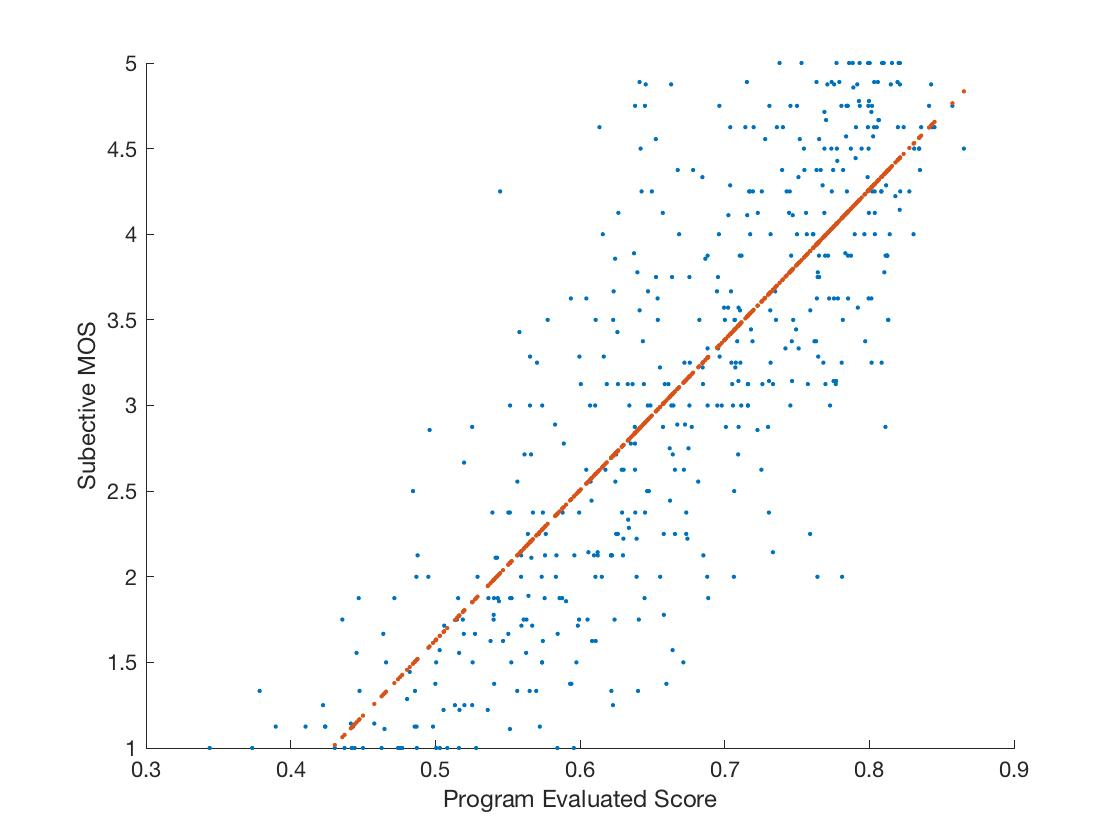
\includegraphics[width=0.8\textwidth]{regress2}
}
\vspace{0.8ex}
\\
\caption{客观评分结果和平均主观意见分的线性回归\label{fig:regress}}
\end{figure}

进一步地,我们使用了两种对比算法对500个短波语音片段进行了客观质量评分。这两种对比算法分别为被ITU-T标准收录的P.563算法和被ANSI标准收录的ANIQUE+算法。我们通过以下几种评价指标来对比本文所提算法和这两种对比算法的表现。

\begin{itemize}
\item Spearman Correlation Coefficient (SCC) - 斯皮尔曼等级相关系数是衡量两个变量的相关性的非参数指标,利用单调方程评价两个统计变量的相关性,取值范围在-1到+1之间,绝对值越接近1说明两个变量相关性越高。通过计算客观评分和主观评分的斯皮尔曼等级相关系数,反应客观评分和主观评分的相关性,绝对值越接近1说明算法效果越好。
\item Root Mean Square Error (RMSE) - 通过计算主观评分MOS分和算法给出的客观评分之间的均方误差大小,直接反映算法评分结果的好坏。RMSE越小说么算法效果越好。
\item Two Class Hit Rate (TCHR) - 选取一个固定阈值将语音分成“优”、“劣”两类,计算通过主观评分分类和通过算法客观评分分类的命中率,即为TCHR结果,越接近1说明算法效果越好。
\end{itemize}

\begin{table}
\centering
\caption{算法性能比较}
\label{tab:alg-compare}
\begin{tabular}{cccc}
\toprule[1.5pt]
算法 & SCC & RMSE & TCHR \\ \midrule[1pt]
本文基于语谱图噪音模型的算法 & 0.87 & 0.58 & 0.89 \\
本文基于自编码器的算法 & 0.82 & 0.69 & 0.82 \\
P.563 & 0.71 & 0.84 & 0.83 \\
ANIQUE+ & 0.43 & 1.08 & 0.71 \\
\end{tabular}
\end{table}

比较结果如表~\ref{tab:alg-compare}所示,从表中数据可见,本文基于语谱图噪音模型的客观评分算法在三种评价指标下的表现都是最优的。而基于自编码器的算法的表现比之略差,但是在SCC和RMSE指标评价下依然优于两种对比算法,TCHR指标略低于P.563算法。

这样的结果符合我们的预期,由于两种对比算法P.563和ANIQUE+没有针对低信噪比的短波语音设计,所以直接应用到短波语音数据上表现并不是很理想。本文提出的基于语谱图噪音模型的客观评分算法,专门针对短波信道的噪音模型进行分析和设计,所以表现最好,但是其适用性较窄,对于预期以外的噪音不能正确评估。而基于自编码器的算法虽然表现略逊一筹,但是其适用性更广,并且能够很方便的迁移应用到其他领域的语音质量评价。

\section{实验B结果}

实验B共进行了20组,每组时长1分钟。如图~\ref{fig:switching-result}所示为两组实验的波形结果,每组实验采集了6路语音信号,其中红色部分表示自动选路的结果,从图中可以看出,自动选路的结果避开了各路信号中噪音很大,波形很乱的时间段,说明自动选路发挥了正常的作用。

\begin{figure}
\centering
\subcaptionbox{实验B示例组1} {
    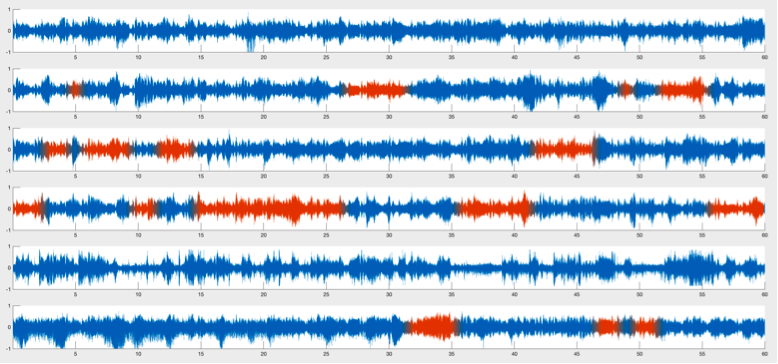
\includegraphics[width=0.8\textwidth]{switching-result1}
}
\vspace{1.2ex}
\\
\subcaptionbox{实验B示例组2} {
    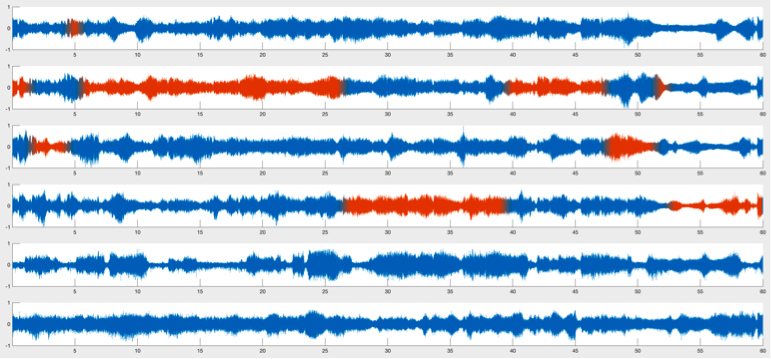
\includegraphics[width=0.8\textwidth]{switching-result2}
}
\vspace{0.8ex}
\\
\caption{实验B输出结果波形\label{fig:switching-result}}
\end{figure}

\begin{figure}
\centering
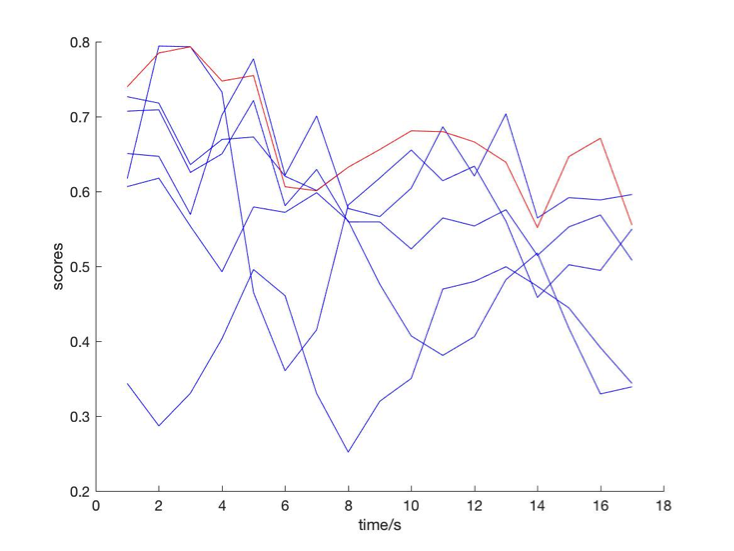
\includegraphics[width=0.45\textwidth]{switching-scores1}
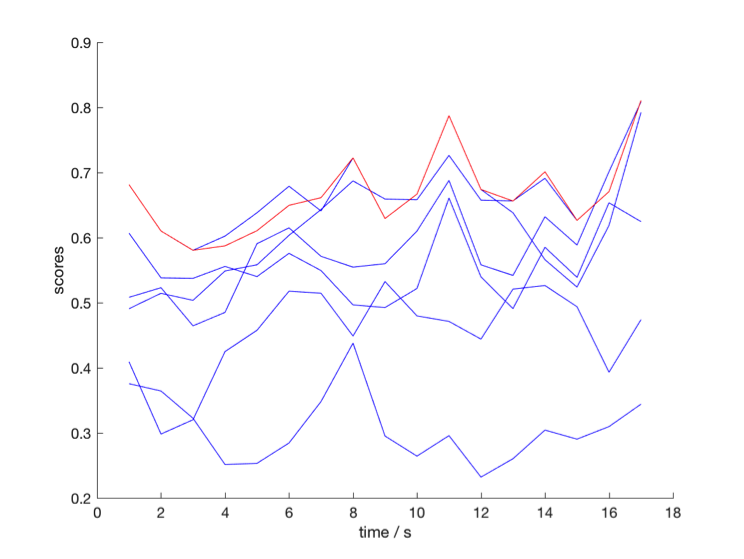
\includegraphics[width=0.45\textwidth]{switching-scores2}
\caption{实验B输出的评分结果\label{fig:switching-scores}}
\end{figure}

对每一组实验结果,我们试听了选路输出的语音和每一路原始语音,比较其主观感受质量。选路输出的语音质量整体要优于各路原始语音信号。我们也试用了客观评分算法对合路语音以及各路语音分时间段进行了客观质量评分,结果如图~\ref{fig:switching-scores}所示。其中红色折线为对选路输出的语音进行评分的结果,而蓝色折线则为各路原始语音的评分结果,从算法客观评分结果来看选路输出的语音质量也是整体最优的。

\section{小结}

本章用实验验证了本文所提算法和系统的效果。实验A中通过分析算法给出的客观评分和人给出的主观评分之间的相关性,验证了本文所提的语音质量客观评价算法在短波语音上有很好的表现。并且我们比较了本文所提算法和两种标准评分算法的结果,诸多指标表明我们的算法在短波语音上有更优秀的表现。实验B中使用本文设计的自动选路系统,对实际多地点接收的短波语音信号进行选路,验证了本文所提系统的功能。实验表明选路输出的语音质量比各路原始语音要好,达到了预想的效果。

% \chapter{果蝇行为识别服务网站的系统设计}

果蝇识别学是动物行为学中的重要组成部分,而自动化的分析果蝇行为对果蝇行为学的研究有重要意义。虽然不同实验室的果蝇研究环境不尽相同,但是果蝇的身体特征相对比较简单、个体之间的差异性并不明显,因而给统一的分析方法提供了可能。在解决了果蝇环境的差异对果蝇行为识别带来的困难后,可以考虑将果蝇行为识别系统推广至其他果蝇拍摄环境。为此,本文专门开发了一个基于果蝇行为识别的网站,通过在网站上提交果蝇视频,并下载识别的结果,实现自动化的果蝇行为识别。果蝇行为识别网站服务方面,主要工作包括两部分:果蝇行为识别程序和网站建设。

\section{果蝇行为识别程序}

果蝇行为识别程序的主要目标在于,通过自动化的果蝇行为分析算法,分析输入的果蝇行为视频,并将分析的结果输出。果蝇行为识别程序希望提供尽可能方便的接口,和灵活可变的配置参数,以便其他程序的调用。下面将介绍果蝇行为识别程序的模块和开发环境。

\subsection{果蝇行为识别的模块结构}

果蝇行为自动化分析主要分为几个模块:活动台的分割、果蝇身体的提取和追踪、果蝇特征的提取、果蝇行为识别。对应到程序中,果蝇行为识别程序主要划分为如图~\ref{fig:fly_detection_procedure2}所示的几个模块,各模块的功能分别如下:
\begin{description}
\item[活动台的分割] 输入包含多个果蝇活动台的视频,输出多个包含单独果蝇活动台的视频,以及对应活动台视频的相关信息,包括:果蝇活动台的中心、果蝇活动台的大小、果蝇活动台移入视频的时间、果蝇活动台移出视频的时间;其中,模块可以输出csv格式的文件,用来保存切分视频的结果;
\item[果蝇身体的提取和追踪] 输入包含单个果蝇活动台的视频,输出果蝇活动台在整个视频中的位置和大小、果蝇身体的尺寸、视频中每一帧果蝇身体和翅膀的区域、每只果蝇身体的轮廓;其中,模型将果蝇的背景模型保存成文件,以方便以后使用;
\item[果蝇特征的提取] 输入果蝇行为视频和果蝇身体提取和追踪模块的结果,输出每一帧中每只果蝇特征点的位置,以及根据果蝇特征点计算得到的果蝇姿态;此外,该模块还可以输出果蝇的速度、加速度等运动信息,并将全部的特征保存到文件;
\item[果蝇行为识别] 输入每只果蝇的位置信息、姿态信息,输出果蝇在整个时间段的行为分析结果。此外,模块还可以输出果蝇行为的特征。
\end{description}

\begin{figure}
\centering
\begin{tikzpicture}
\node [block, text width=10em] (split_chambers) {\heiti 果蝇活动台分割};
\node [block, text width=10em, below = 0.5cm of split_chambers] (extract_contour) {\heiti 果蝇身体轮廓提取};
\node [block, text width=10em, below = 0.5cm of extract_contour] (feature_extract) {\heiti 果蝇特征提取};
\node [block, text width=10em, below = 0.5cm of feature_extract] (behavior_detect) {\heiti 果蝇行为分析};

\path [arrow] (split_chambers) -- (extract_contour);
\path [arrow] (extract_contour) -- (feature_extract);
\path [arrow] (feature_extract) -- (behavior_detect);
\end{tikzpicture}
\caption{果蝇行为识别自动化分析流程}
\label{fig:fly_detection_procedure2}
\end{figure}

\subsection{果蝇行为识别程序的开发和编译环境}

果蝇行为识别程序主要部署在Linux操作系统下,其开发环境的主要依赖关系包括:
\begin{itemize}
\item OpenCV 2.4.x
\item CMake >= 3.0
\end{itemize}

OpenCV被广泛的应用在果蝇行为识别程序中\cite{itseez2015opencv,itseez2014theopencv}。OpenCV的全称Open Source Computer Vision Library,是一个免费、开源的计算机视觉方面的库,该库以BSD开源软件协议发布,提供了大量的计算机图形学中的基本操作接口,如视频、图像的IO操作、基础的图形学操作如色域转换、高级的图像特征算法如方向梯度直方图(Histogram of oriented gradient,HOG)算法\cite{dalal2005histograms}、尺度不变特征变换(Scale-invariant feature transform,SIFT)算法\cite{lowe1999object}等,以及部分计算机学习库,如SVM等。此外,OpenCV还兼容不同的平台,可以方便的部署到Windows、Linux等系统上。本文使用了稳定版本的OpenCV 2.4.x,主要利用OpenCV库提供的图形学操作进行图形的基本处理,以及机器学习库进行测试等。

对于果蝇行为识别程序而言,果蝇行为视频的处理大概能做到接近实时,即程序运行的时和果蝇视频的长度在同一个量级。和其他果蝇行为分析系统相比,该程序的运行速度并不算慢\cite{dankert2009automated},但是仍然存在较大的发展空间。对于一个摄像头,一般会同时拍摄超过20个果蝇活动台,这就给程序处理带来较大的压力。为此,在维持现有算法基本不变的情况下,可以从OpenCV库的选择入手。目前,OpenCV的最新稳定版本为 2.4.13,但是最新的开发版本已经到了 3.2.0。最新的3.2.0版本除了提供更开放的计算机图形学算法外,还为大部分的计算机图形学操作、矩阵运算等提供了GPU运算接口,对于大量的计算机图形学操作,可以大大提高程序运行的效率。

在程序的编译方面,使用CMake作为程序的make工具,并使用gcc编译器,对果蝇行为识别程序。编译完成后,得到可执行程序DetectFly,通过命令行参数指定输入的视频、果蝇行为视频的类型(打架、求偶)、输出结果的文件名等。可执行程序通过分析果蝇视频,将果蝇的行为输出到特定的文件中。外部程序可以通过调用可执行程序,得到果蝇行为视频中果蝇的所有行为。

\section{果蝇行为识别网站}

在果蝇行为自动分析程序DetectFly的基础上,本文搭建了果蝇行为自动分析的网站,对外提供果蝇行为识别服务。果蝇行为识别网站提供了用户注册、用户登录、果蝇行为识别任务的添加、果蝇行为识别任务结果下载等功能。下面简单介绍果蝇行为识别的自动化分析网站。

\subsection{网站的功能介绍}

果蝇行为识别网站的链接:\url{http://gu.ee.tsinghua.edu.cn/drosophila}。目前,网站主要包含以下功能:用户的注册、用户登录、果蝇行为视频任务的创建、果蝇行为视频上传、果蝇行为视频分析结果下载等模块。

果蝇行为识别网站存在用户管理功能。果蝇行为识别需要大量的计算资源,因而对用户的使用需要一定的条件,以便进行资格审查。首先,需要用户进行注册,只有注册用户才能使用网站提供的果蝇行为识别功能。网站的注册页面如图~\ref{fig:website_register}所示,用户需要提供包括姓名、研究机构、电子邮箱等基本信息,以便进一步联系。

\begin{figure}
\centering
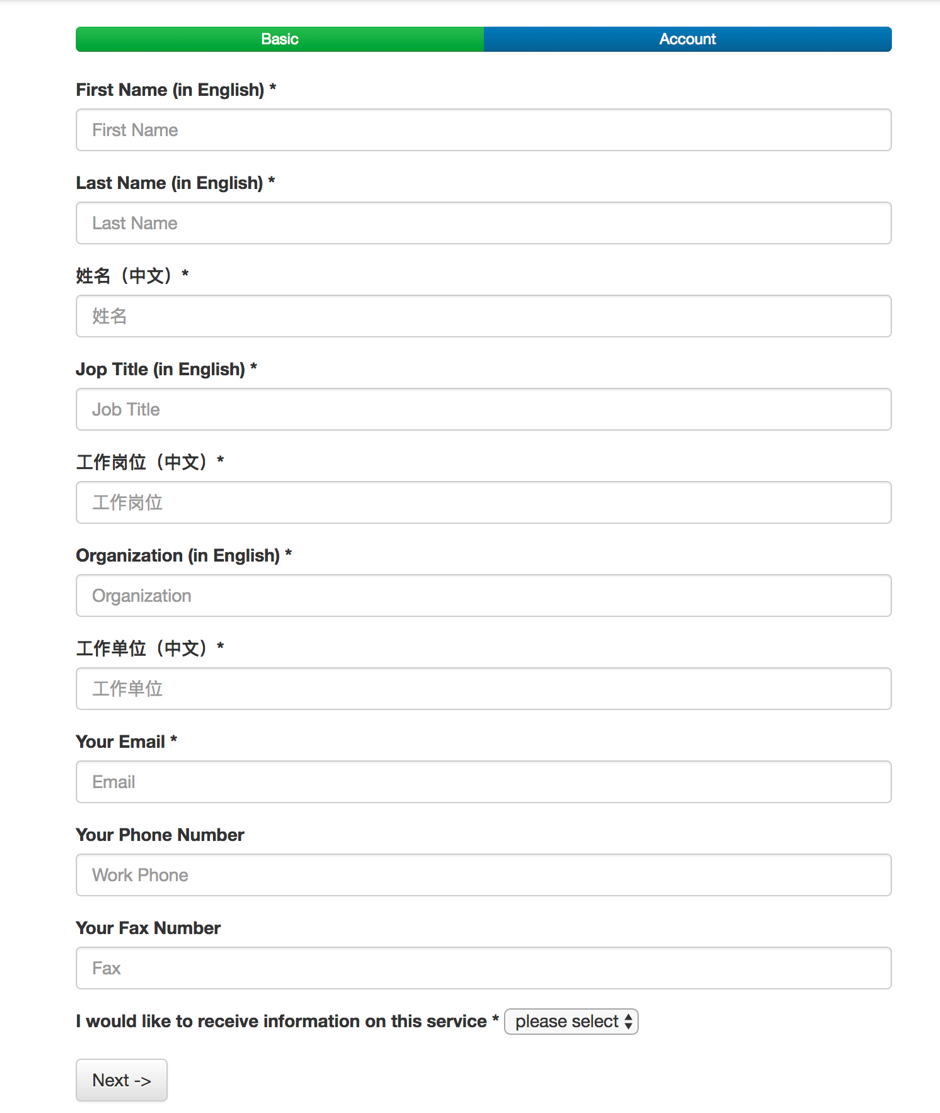
\includegraphics[width=0.8\textwidth]{website_register}
\caption{果蝇行为识别网站的注册}
\label{fig:website_register}
\end{figure}

在用户提交注册申请后,网站后台会给管理员发送邮件,等待管理员确认用户资格后,用户可以正常登陆和使用网站提供的果蝇行为识别服务。网站的登录页面如图~\ref{fig:website_login}所示。

\begin{figure}
\centering
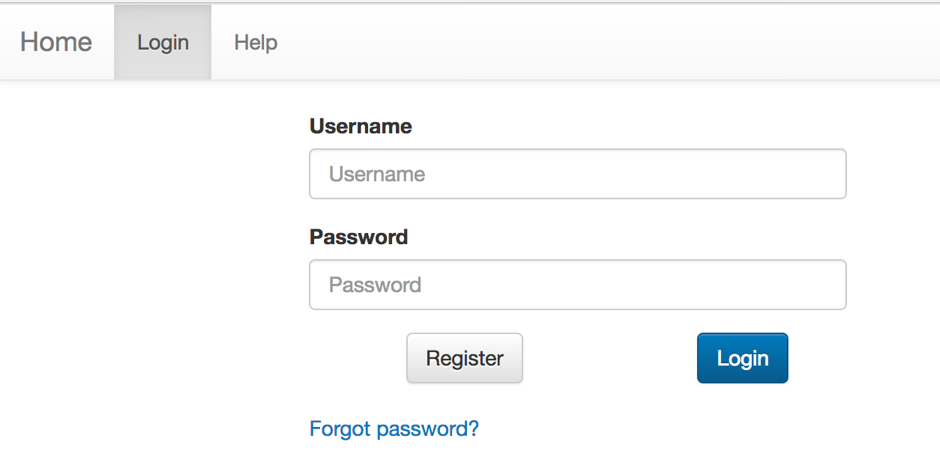
\includegraphics[width=0.8\textwidth]{website_login}
\caption{果蝇行为识别网站的登录}
\label{fig:website_login}
\end{figure}

完成登录后,可以创建果蝇行为识别任务,并上传果蝇行为视频。图~\ref{fig:website_new_mission}界面显示了创建果蝇行为识别任务的界面,目前,网站支持2种果蝇行为识别任务:打架行为和求偶行为。创建任务时,需要选定果蝇行为识别的任务类型、创建的任务名称,还支持对任务进行简单的评注,以便日后查找。对于已经完成的任务,还提供了不同的过滤列表,以便用户查询。过滤列表有以下4种:
\begin{itemize}
\item All - 全部任务列表
\item Failed - 失败的任务列表
\item Succeeded - 成功的任务列表
\item Incomplete - 未完成任务列表
\end{itemize}

\begin{figure}
\centering
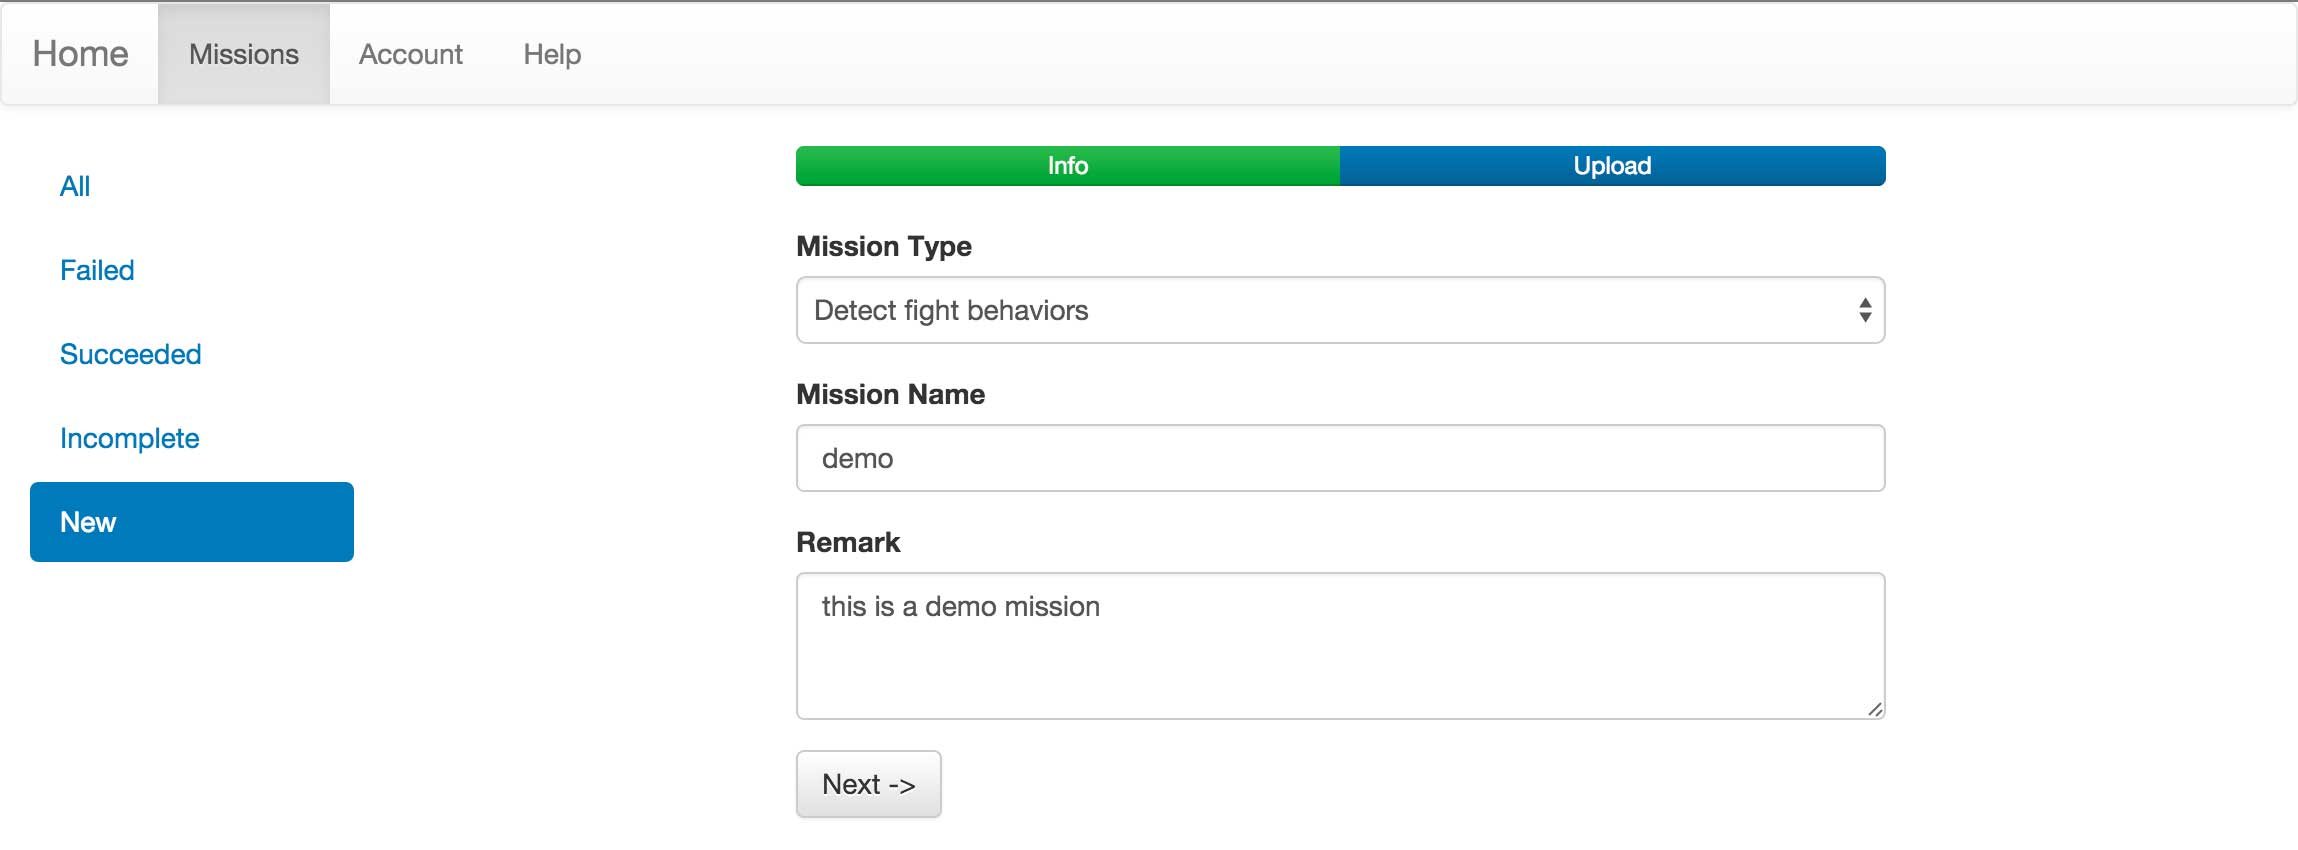
\includegraphics[width=0.8\textwidth]{website_new_mission}
\caption{创建果蝇行为识别任务}
\label{fig:website_new_mission}
\end{figure}

在完成任务创建后,需要上传果蝇行为视频。果蝇行为视频文件的大小较大,此步骤需要花费一定时间。一般来说,错误的果蝇活动台分割会给后续的果蝇行为识别任务带来难以预计的结果,这会给网站带来大量无用的计算,并消耗用户大量的时间。在综合考虑后,网站要求用户自行进行果蝇活动台的分割任务,同时要求上传的果蝇行为视频为包含一个单独的果蝇活动台的果蝇行为视频。如图~\ref{fig:website_new_mission}所示,视频文件上传完成后,点击"submit"即可提交果蝇分析任务。任务状态[Mission State]会有如下几种:
\begin{itemize}
\item Pending – 任务正在等待被处理
\item Processing – 任务正在处理中(这一步是计算过程,需要等待较长时间)
\item Succeeded – 任务处理完成
\item Failed – 任务处理失败
\end{itemize}

\begin{figure}
\centering
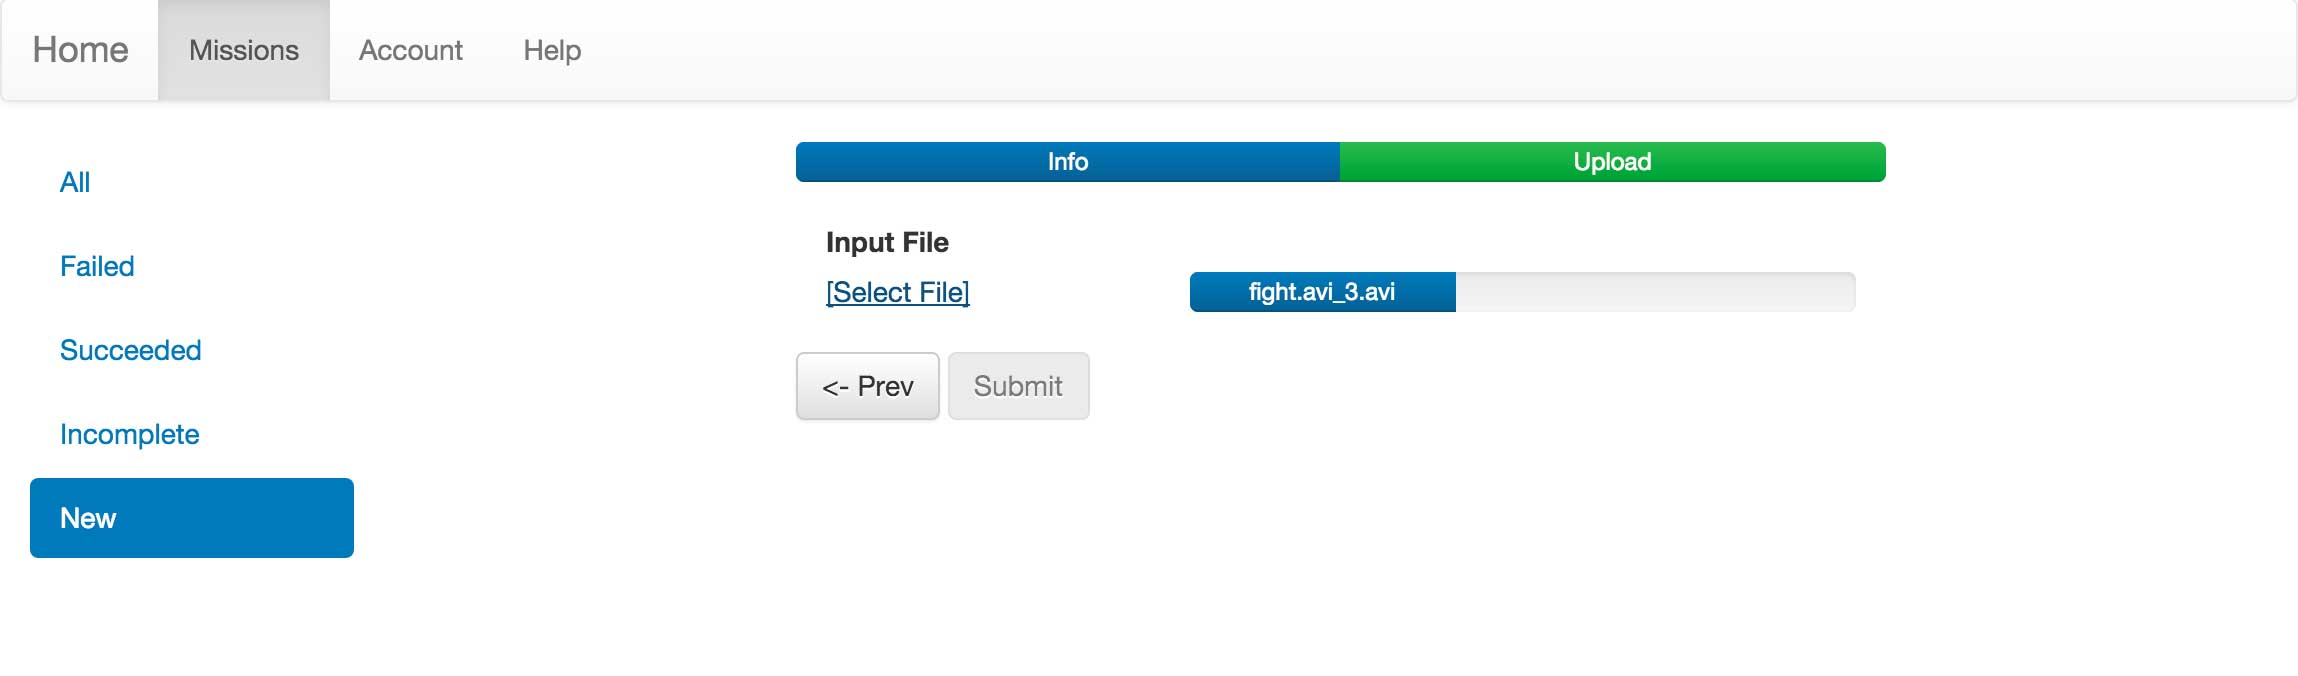
\includegraphics[width=0.8\textwidth]{website_upload_video}
\caption{上传果蝇行为视频}
\label{fig:website_upload_video}
\end{figure}

在此阶段,用户看到如图~\ref{fig:website_waiting_for_result}界面。

\begin{figure}
\centering
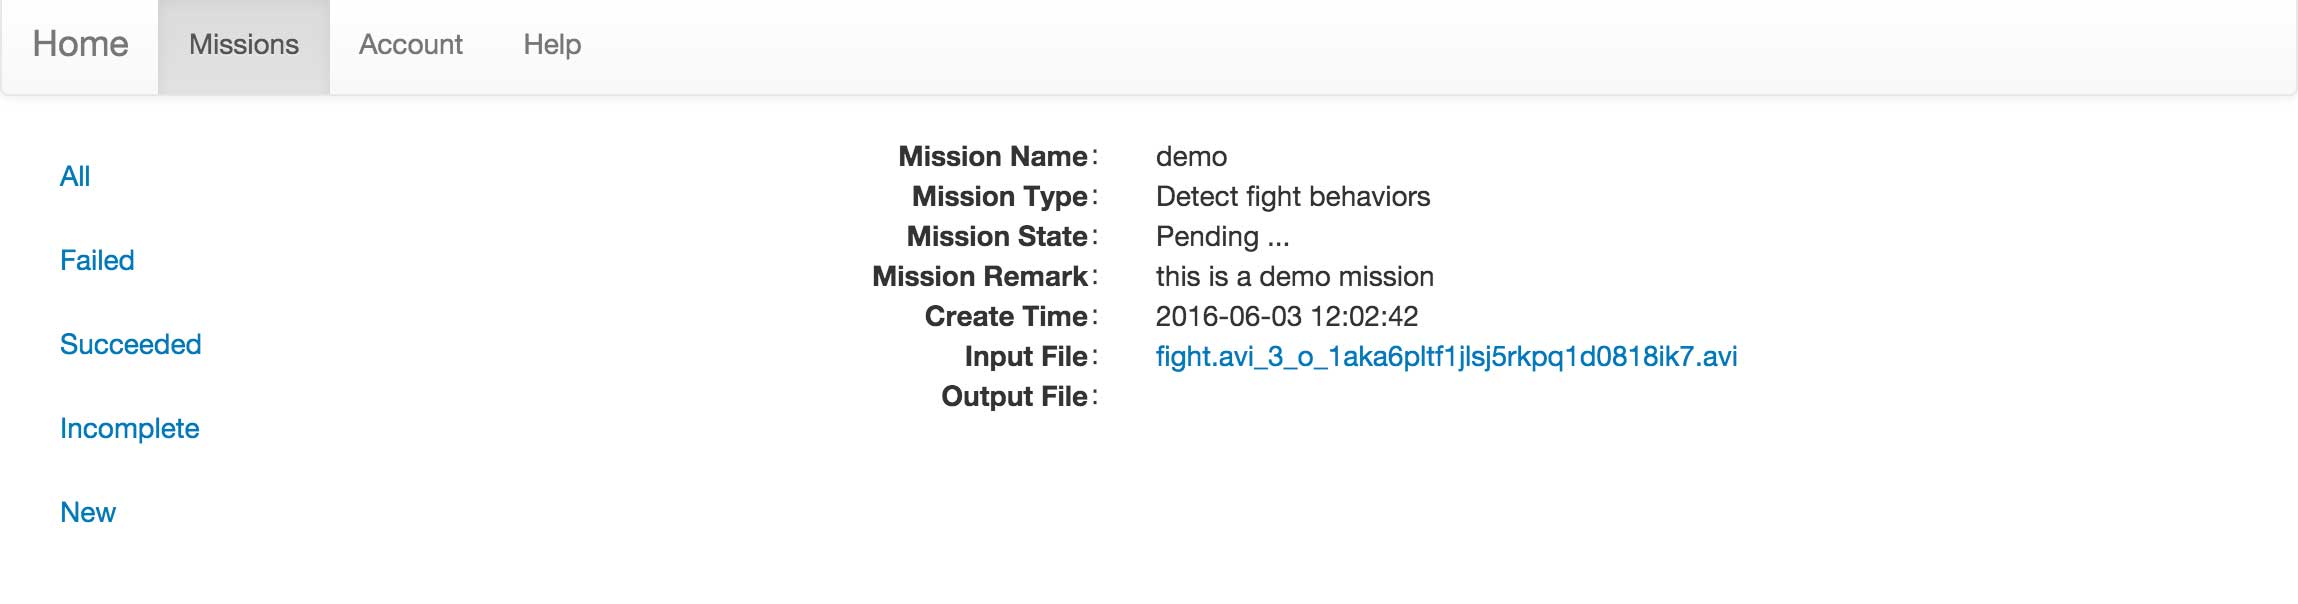
\includegraphics[width=0.8\textwidth]{website_waiting_for_result}
\caption{等待任务完成}
\label{fig:website_waiting_for_result}
\end{figure}

最后,经过任务队列的等待后,网站后台对任务进行分析,得到果蝇行为识别的结果,如图~\ref{fig:website_show_result}所示。

\begin{figure}
\centering
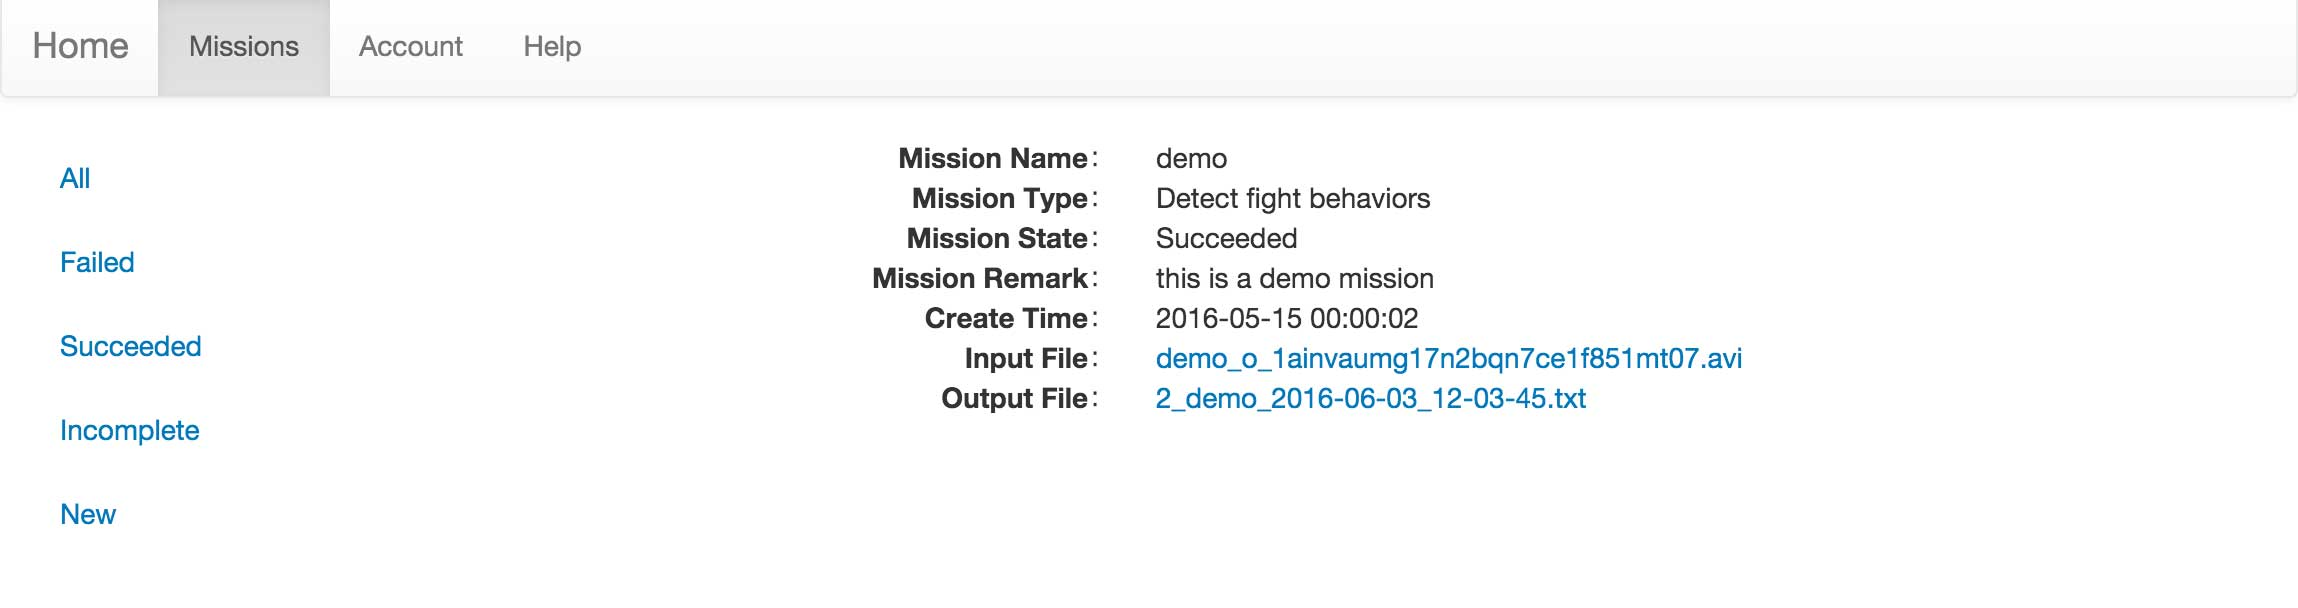
\includegraphics[width=0.8\textwidth]{website_show_result}
\caption{果蝇行为识别任务的结果}
\label{fig:website_show_result}
\end{figure}

图~\ref{fig:website_show_result}中,"Output File"栏目对应的就是果蝇行为识别的结果,即果蝇打架日志。对于不同类型的果蝇行为分析任务,其日志输出有不同的格式。对于打架行为,日志的第一行统计了视频中果蝇的打架次数,其后有以下3列:
\begin{itemize}
\item time – 打架发生的时间
\item frame – 打架发生的帧数,和time对应(从零开始)
\item strength – 打架强度
\end{itemize}
对于果蝇的求偶行为,求偶行为包括果蝇的身体求偶行为和振翅求偶行为,日志的第一行统计了视频中的求偶行为总数,其后有以下4列:
\begin{itemize}
\item time – 求偶起始时间
\item start – 求偶起始帧(含)
\item end – 求偶结束帧(含)
\item behavior – 求偶行为
\end{itemize}

除基本的日志外,果蝇求偶行为分析日志文件还输出简单的统计信息。在输出身体求偶或振翅求偶行为后,日志输出各求偶行为的持续时间,包括:
\begin{itemize}
\item count – 行为总发生次数
\item duration – 行为总持续时间
\end{itemize}
最后,日志输出行为间的转移矩阵,其第$i$行第$j$列表示从第$j$个行为向第$i$个行为转移的次数,单位为帧。用户通过下载果蝇行为日志文件,并按照既定格式进行分析,得到果蝇行为的各项参数,用于支持果蝇行为学的研究。

\subsection{果蝇行为识别网站简介}

网站建设在Ubuntu 14.04系统上,操作系统的选择主要考虑了果蝇行为识别程序的发布、网站服务的搭建等,最后综合选取了Ubuntu 14.04操作系统。网站的基本环境要求如下:
\begin{itemize}
    \item 操作系统:Ubunutu 14.04
    \item Web服务器: Apache2,支持PHP
    \item PHP: >=5.2.4
    \item 数据库:MySQL 5.5
    \item Python: 2.7.x
\end{itemize}

网站部分使用CodeIgniter框架搭建。CodeIgniter是一个轻量级的MVC架构的php网站框架,基于MVC模型,将网站的应用层和逻辑层进行分离\cite{burbeck87}。关于后台的数据库,系统使用MySQL数据库存储数据,主要存储了包括用户账户相关的数据表、任务类型数据表、任务数据表等,分别参见表~\ref{tab:account}、表~\ref{tab:mission_type}和表~\ref{tab:misson}。

\begin{table}
\centering
\caption{账户信息数据表dp\_account}
\label{tab:account}
\begin{tabular}{ccc}
\toprule[1.5pt]
字段名 & 字段类型 & 备注 \\ \midrule[1pt]
aid & bigint(20) & Unsigned, Primary key, Auto Increment \\
state & tinyint(4) & 0:等待审核,1:正常,2:禁用 \\
username & varchar(20) & 用户名 \\
password & varchar(32) & 密码的md5 \\
work\_unit & varchar(255) & 学校/单位 \\
department & varchar(255) & 院系 \\
purpose & varchar(255) & 实验目的 \\
source & varchar(255) & 项目来源 \\
data\_amount & varchar(255) & 数据量 \\
create\_time & timestamp & 默认current\_timestamp \\ \bottomrule[1.5pt]
\end{tabular}
\end{table}

\begin{table}
\centering
\caption{任务类型数据表dp\_missiontype}
\label{tab:mission_type}
\begin{tabular}{ccc}
\toprule[1.5pt]
字段名 & 字段类型 & 备注 \\ \midrule[1pt]
mtid & int(10) & Unsigned, Primary key, Auto Increment \\
state & tinyint(3) & 0:Invalid, 1:Valid \\
typename & varchar(255) & 类型名称 \\
description & varchar(1000) & 类型说明 \\
command & varchar(255) & 处理命令,可以加入特殊符号,具体见下表 \\
in\_file\_exts & varchar(255) & 允许的输入文件后缀,逗号分隔 \\
out\_file\_ext & varchar(10) & 输出文件的后缀 \\
max\_in\_file\_size & varchar(20) & 允许上传的输入文件大小 \\
error\_messages & varcahr(1000) & json格式字符串,各个error\_code的含义 \\ \bottomrule[1.5pt]
\end{tabular}
\end{table}

\begin{table}
\centering
\caption{任务数据表dp\_mission}
\label{tab:misson}
\begin{tabular}{ccp{0.5\columnwidth}}
\toprule[1.5pt]
字段名 & 字段类型 & 备注 \\ \midrule[1pt]
mid & bigint(20) & Unsigned, Primary key, Auto Increment \\
aid & bigint(20) & 所属account的aid \\
type & mediumint(6) & 任务类型的id,对应dp\_missiontype中的mtid \\
name & varchar(20) & 任务名称 \\
remark & varchar(1000) & 任务备注 \\
state & smallint(6) & {任务状态,
\begin{itemize}
    \item 0 : Pending等待处理
    \item 1 : Proceeding处理中
    \item 2 : Succeeded
    \item 3 : Failed
\end{itemize}} \\
error\_code & int(11) & 错误码,状态为Failed时有效 \\
in\_file\_path & varchar(255) & 输入文件路径,相对于项目根目录 \\
out\_file\_path & varchar(255) & 输出文件路径,相对于项目根目录,状态为Succeeded时有效 \\
stdout\_file\_path & varchar(255) & 处理过程的stdout日志文件路径,相对于项目根目录,状态为Succeeded/Failed时有效 \\
stderr\_file\_path & varchar(255) & 处理过程的stderr日志文件路径,相对于项目根目录,状态为Succeeded/Failed时有效 \\
create\_time & timestamp & 创建时间,默认current\_timestamp \\
complete\_time & datetime & 完成时间,状态为Succeeded/Failed时有效 \\
\bottomrule[1.5pt]
\end{tabular}
\end{table}

任务处理使用Python脚本实现,并用Supervisor管理脚本的执行。Supervisor是一个基于Python的进程管理系统,可以方便的进行任务的创建、监听、重启、崩溃恢复等,经过简单的配置后,可以用Supervisor进行任务队列的管理,安排果蝇自动检测程序DetectFly对果蝇视频的任务队列进行逐个分析和处理。通过为不同的任务类型指定不同的命令行参数,调用DetectFly程序,完成果蝇行为的识别,并将行为识别的结果保存为日志文件,方便用户下载和分析。

\section{小结}

在Ubuntu下配置开发环境,得到果蝇行为自动识别的可执行程序DetectFly。DetectFly可以通过命令行参数,实现不同类型的果蝇行为识别。在CodeIgniter框架的基础上,使用Supervisor进行任务队列管理,最终实现了果蝇行为识别网站的任务管理。


% \chapter{总结与展望}

\section{论文工作总结}

动物行为学是生物学研究中的重要领域,而果蝇行为学是动物行为学中的一个分支。果蝇因其形态简单等原因,可以通过计算机视觉、机器学习等相关领域的技术对果蝇进行自动识别。本文为了提高果蝇行为识别对视频拍摄环境变化的鲁棒性,针对果蝇行为识别的果蝇活动台分割和果蝇身体轮廓提取部分进行研究,并以网站的形式提供果蝇行为检测服务。下面是本文的主要工作和创新点。

首先,果蝇活动台的分割操作一般通过对形态学上检测来完成,匹配的检测果蝇活动台的形状来提取果蝇活动台的位置。为了适应不同果蝇行为视频的差异,本文通过对形态学操作中的参数控制形检测到的形状的数目,并对参数进行自适应,提高了果蝇活动台匹配算法的适用性。同时,针对特定排列的果蝇活动台,通过对活动台的实际坐标和理想坐标之间建立仿射变换,提高了果蝇活动台位置的准确性。

其次,针对果蝇身体轮廓提取算法,本文在背景模型的基础上,通过对果蝇视频背景进行首次建模,得到初步的果蝇身体和翅膀提取算法,进而通过分离果蝇身体和翅膀,实现对果蝇活动台的单独建模,得到精确的果蝇活动台模型。上述背景模型显著提高了果蝇身体轮廓提取的鲁棒性,在不同的果蝇行为视频中表现出相当的鲁棒性。

最后,通过搭建网站,提供果蝇行为识别的服务,可以方便不同研究人员使用相关的服务。

\section{未来工作展望}

基于本文开展的工作,将来的工作可以有以下几个考量:

\begin{enumerate}
\item 目前,本文仅针对果蝇活动台分割和果蝇身体轮廓提取部分进行了充分的实验,对于背景模型和果蝇行为识别的准确率之间的关系,受限于标定的果蝇视频的规模,目前还没有完全展开,希望以后能进一步在其他果蝇行为视频的数据上加以推广、验证。
\item 果蝇活动台分割算法的准确性还有待提高。对于排列不规则的果蝇活动台,对果蝇活动台中心进行聚类时偶尔会出现部分活动台被重复定位、部分活动台没有被准确定位到的问题,算法运行的结果还需要手工进行确认。
\item 果蝇行为分析的效率还存在提升的空间,目前在算法层面上可以改进的空间相对不多,可以用GPU运算等方式提高检测程序的处理能力。
\item 可以将对果蝇的背景模型等研究加以推广,应用到其他类型的研究中。
\end{enumerate}


%%% 其它部分
\backmatter

%% 本科生要这几个索引,研究生不要。选择性留下。
% 插图索引
% \listoffigures
% 表格索引
% \listoftables
% 公式索引
% \listofequations


%% 参考文献
% 注意:至少需要引用一篇参考文献,否则下面两行可能引起编译错误。
% 如果不需要参考文献,请将下面两行删除或注释掉。
\bibliographystyle{thuthesis}
\bibliography{ref/refs}

%% 致谢
\begin{acknowledgement}

我要感谢我的导师谷源涛老师,在我的研究生学习期间,谷老师在我的学术研究上给予了充分的指导,帮助我在自己的研究上有充分的发挥。同时,谷老师对我的职业规划和发展方向也给予了很多的建议和帮助,让我受益匪浅。此外,谷老师严谨求实的工作作风,勤奋认真的工作态度都潜移默化地感染了我。谷老师对于我的论文工作也提供了诸多指点和帮助,在此我要向谷老师表示由衷的感谢。

我要感谢实验室的各位同学,他们抽出宝贵的时间,帮助我对论文中的实验语音进行了主观质量标注。尤其要感谢刘雄飞同学,他参与了很多短波语音的采集工作,非常枯燥耗时,但对于本文工作又是至关重要的。

我还要感谢我的父母、家人和朋友。他们对我的关心和支持给了我不断突破自我的动力,特别要感谢段泽群同学一直以来的陪伴与关心。

\end{acknowledgement}


%% 附录
% \begin{appendix}
% \input{data/appendix01}
% \end{appendix}

%% 个人简历
\begin{resume}

\resumeitem{个人简历}

1994年2月4日生于江苏省淮安市。

2011年9月通过竞赛保送进入 清华大学 电子工程系 电子信息科学与技术专业,2015年7月本科毕业,并获得了工学学士学位,同时获得免试攻读 清华大学 电子工程系 工学硕士学位资格。

2015年9月面试进入 清华大学 电子工程系 攻读 信息与通信工程专业 工学硕士学位 至今。

\researchitem{学术论文发表情况}

\begin{publications}
\item Ye Chen, Yongcheng Wang, Jiaguo Yang, Yuantao Gu. Automatic Switching Technique for Speech Enhancement in HF Communications. IEEE 8th International Conference on Electronics Information and Emergency Communication (已录用,EI)
\item 谷源涛,陈晔. 语音质量评价方法及装置. (已申请,专利)
\end{publications}

\end{resume}

\end{document}
